\documentclass{article}

\usepackage[colorlinks, urlcolor=blue, linkcolor=red, citecolor=green]{hyperref}
\usepackage{fancyhdr} %设置页眉和页脚的
\usepackage{extramarks} %设置continue那玩意的
\usepackage{amsmath}
\usepackage{amsthm}
\usepackage{amsfonts}
\usepackage{tikz} %画线的
\usepackage[plain]{algorithm}
\usepackage{algpseudocode}
\usepackage{enumerate}

\usetikzlibrary{automata,positioning}

%表
\usepackage{booktabs}
\usepackage{multirow}
\usepackage{array}
\usepackage{caption}
\DeclareCaptionFont{heiti}{\heiti} %还可以定义其他的
\captionsetup{labelsep=space, font={small, bf}, skip=2pt} %space可以改成quad

%图
%*****************图片及其相关设置***************************
\usepackage{graphicx}
\graphicspath{{tupian/}}
\usepackage{subfigure}
%
% Basic Document Settings
%

\topmargin=-0.45in
\evensidemargin=0in
\oddsidemargin=0in
\textwidth=6.5in
\textheight=9.0in
\headsep=0.25in

\linespread{1.1}

\pagestyle{fancy}
\lhead{\hmwkAuthorName}
\chead{\hmwkClass: \hmwkTitle}
\rhead{\firstxmark}
\lfoot{\lastxmark}
\cfoot{\thepage}

\renewcommand\headrulewidth{0.4pt}
\renewcommand\footrulewidth{0.4pt}

\setlength\parindent{0pt}

%
% Create Problem Sections
%

\newcommand{\enterProblemHeader}[1]{
    \nobreak\extramarks{}{Assignment A1.\arabic{#1} continued on next page\ldots}\nobreak{}
    \nobreak\extramarks{Assignment A1.\arabic{#1} (continued)}{Assignment A1.\arabic{#1} continued on next page\ldots}\nobreak{}
}

\newcommand{\exitProblemHeader}[1]{
    \nobreak\extramarks{Assignment A1.\arabic{#1} (continued)}{Assignment A1.\arabic{#1} continued on next page\ldots}\nobreak{}
    \stepcounter{#1}
    \nobreak\extramarks{Assignment A1.\arabic{#1}}{}\nobreak{}
}

\setcounter{secnumdepth}{0}
\newcounter{partCounter}
\newcounter{homeworkProblemCounter}
\setcounter{homeworkProblemCounter}{1}
\nobreak\extramarks{Assignment A1.\arabic{homeworkProblemCounter}}{}\nobreak{}

\newenvironment{homeworkProblem}{
    \section{Assignment A1.\arabic{homeworkProblemCounter}}
    \setcounter{partCounter}{1}
    \enterProblemHeader{homeworkProblemCounter}
}{
    \exitProblemHeader{homeworkProblemCounter}
}

%
% Homework Details
%   - Title
%   - Due date
%   - Class
%   - Section/Time
%   - Instructor
%   - Author
%

\newcommand{\hmwkTitle}{Homework\ \#1}
\newcommand{\hmwkDueDate}{October 10, 2020}
\newcommand{\hmwkClass}{Introduction to Optimization}
\newcommand{\hmwkClassTime}{}
\newcommand{\hmwkClassInstructor}{Professor Andre Milzarek}
\newcommand{\hmwkAuthorName}{Peng Deng}
\newcommand{\hmwkAuthorSchool}{School of Data Science}
\newcommand{\hmwkAuthorNumber}{Sno.220041042}
%
% Title Page
%

\title{
    \vspace{2in}
    \textmd{\textbf{\hmwkClass:\ \hmwkTitle}}\\
    \normalsize\vspace{0.1in}\small{Due\ on\ \hmwkDueDate}\\
    \vspace{0.1in}\large{\textit{\hmwkClassInstructor\ \hmwkClassTime}}
    \vspace{3in}
}

\author{\textbf{\hmwkAuthorName}}

\date{}

\renewcommand{\part}[1]{\textbf{\large Part \Alph{partCounter}}\stepcounter{partCounter}\\}

%
% Various Helper Commands
%

% Useful for algorithms
\newcommand{\alg}[1]{\textsc{\bfseries \footnotesize #1}}

% For derivatives
\newcommand{\deriv}[1]{\frac{\mathrm{d}}{\mathrm{d}x} (#1)}

% For partial derivatives
\newcommand{\pderiv}[2]{\frac{\partial}{\partial #1} (#2)}

% Integral dx
\newcommand{\dx}{\mathrm{d}x}

% Alias for the Solution section header
\newcommand{\solution}{\textbf{\large Solution}}

% Probability commands: Expectation, Variance, Covariance, Bias
\newcommand{\E}{\mathrm{E}}
\newcommand{\Var}{\mathrm{Var}}
\newcommand{\Cov}{\mathrm{Cov}}
\newcommand{\Bias}{\mathrm{Bias}}
\begin{document}

\maketitle
\thispagestyle{empty}

\newpage
\setcounter{page}{1}

\begin{homeworkProblem}
	A local family-owned plastic cup factory wants to optimize its production mix in order to maximize its profit. The factory produces personalized beer mugs and champagne glasses. The profit on a box of beer mugs is 200 RMB while the profit on a box of champagne glasses is 150 RMB.
	
	\vspace{4pt}
	The cups are manufactured with a machine called a plastic extruder which feeds on plastic resins. Each box of beer mugs requires 9 kg of plastic resins to produce while champagne glasses require 5.5 kg per box. The daily supply of plastic resins is limited to at most 900 kg. About 15 boxes of either product can be produced per hour. At the moment the family wants to limit their work day to 8 hours.
	
	\vspace{4pt}
	Write an optimization problem to maximize the profit of this company.
	
	\vspace{8pt}
	\textbf{\large{Solution}}
	
	Firstlt, we set the company produce $x$ boxes beer mugs and $ y $ boxes champagne glasses. Thus we can get the follow definition.
	
	\vspace{4pt}
	$\circ$ \textbf{Decisions variable:} the number of boxes of beer mugs $x$ and the umber of boxes of beer mugs $y$.
	
	$\circ$ \textbf{Objective:} maximize the profit $f(x,y) = 200x+150y$.
	
	$\circ$ \textbf{Constraints:} 
	
	\hspace{10pt}1)The total use of plastic resins: $9x+5.5y\le900$.
	
	\hspace{10pt}2)The total boxes of beer mugs and champagne glasses: $x+y\le(15)(8)=120$.
	
	\hspace{10pt}3)The boxes of beer mugs and champagne glasses should greater than or equal to zero: $x \ge 0, y\ge0$, and must be integers.
	
	\vspace{4pt}
	Then we solve the optimization problem by drawing the linear programming graph as Figure \ref{coordinate1}. As we can see from Figure \ref{coordinate1}, the red dash line is the profit function with variable profits. And the points in the blue area are the available decisions. So we can find the maximum of profit near the point $ C(x=68.57, y=51.43) $. Because the boxes should be integers, finally we can find the maximum of profit as $ x=68, y=52 $, and the maximum of profit is
	\begin{equation}
		f(x,y)_{max} = 200x+150y= (200)(68)+(150)(52)=21400
	\end{equation}
	
	\begin{figure}[htbp]
		\centering
		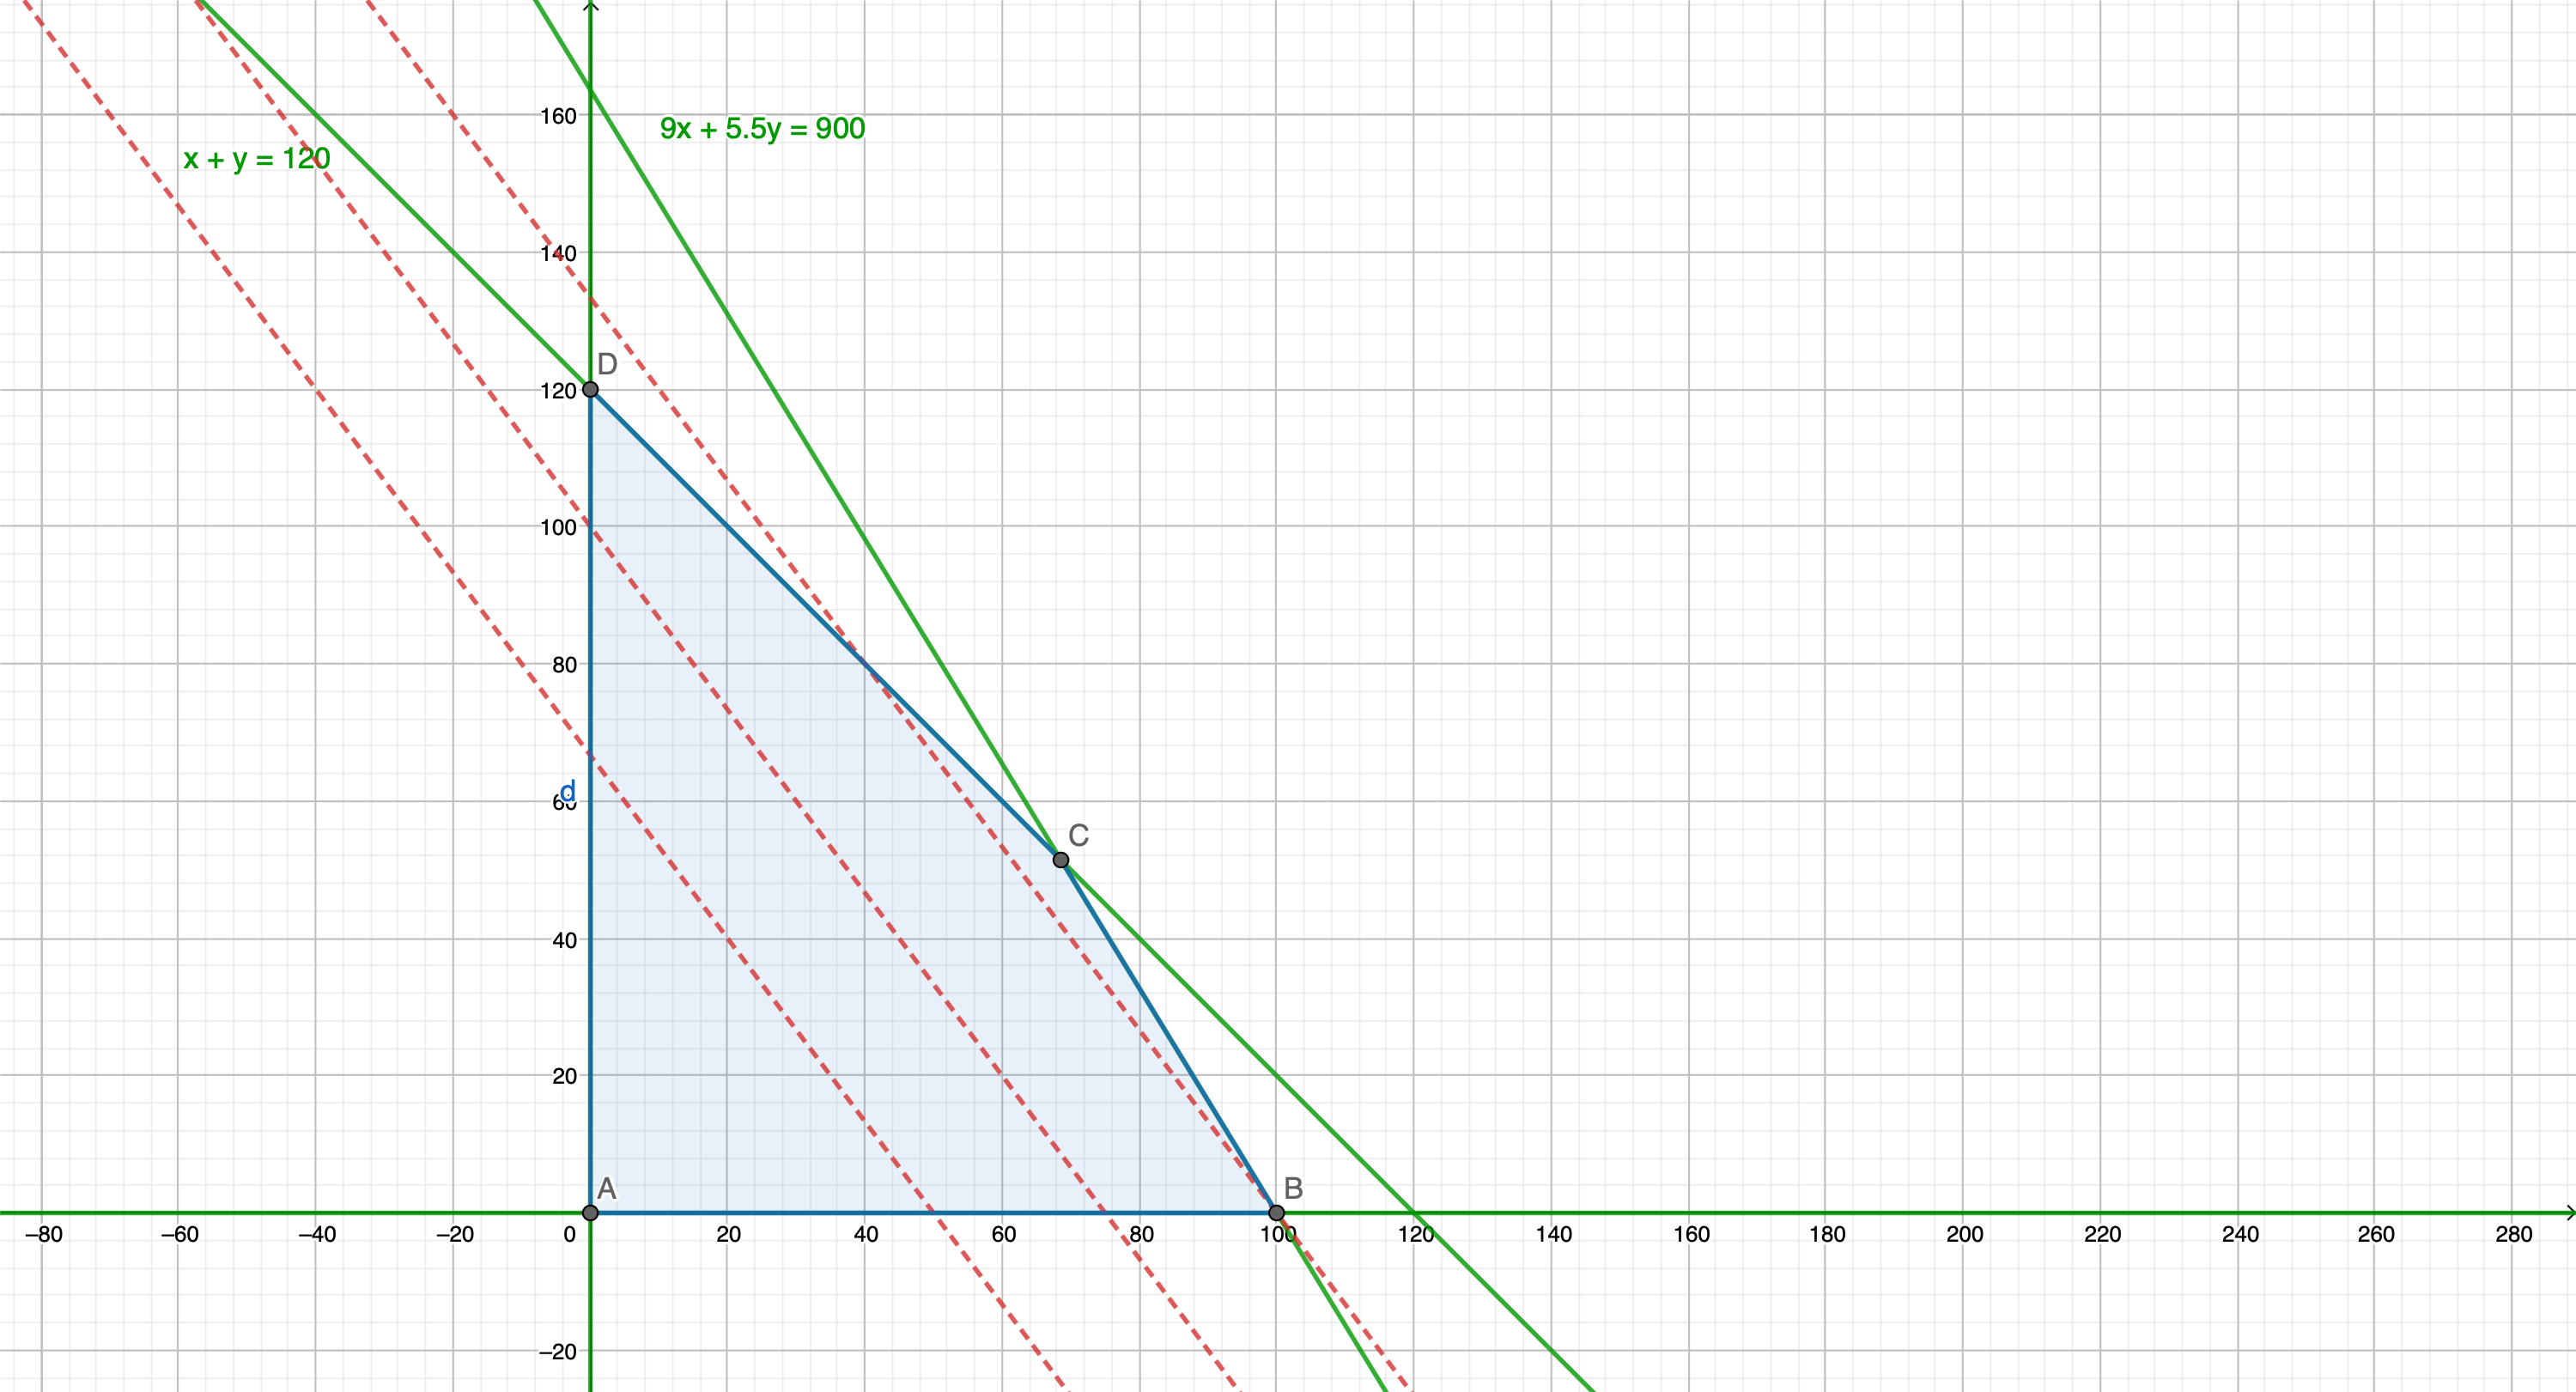
\includegraphics[width=0.8\linewidth]{image1}
		\vspace{4pt}
		\caption{Linear programming of the factory profit}
		\label{coordinate1}
	\end{figure}
\end{homeworkProblem}
\pagebreak

\begin{homeworkProblem}
	A local brewery produces Ale and Beer. The production is currently limited by the available resources of corn, hops, and barley malt. To produce one box of Ale 5 kg of corn, 4 kg of hops and 35 kg of malt are required. To make one box of Beer 15 kg of corn, 4 kg of hops, and 20 kg of malt are required. Suppose that only 480 kg of corn, 160 kg of hops and 1190 kg of malt are available.
	\begin{enumerate}[a)]
		\item Formulate a linear program (= linear optimization problem) to maximize the profit of the brewery when one box of Ale achieves a profit of 130 RMB and one box of Beer achieves a profit of 230 RMB.
		\item The brewery also wants to consider time constraints. The production of one box of Ale requires 1.5 hours while the production of one box of Beer requires 2.5 hours. The two production processes can not run at the same time and the brewery can only run for up to 12 hours each day.
		
		Revise the linear program from part a) and include these time constraints in an appropriate way to find an optimal production plan for one week of production.
	\end{enumerate}

	\vspace{4pt}
	\textbf{\large{Solution}}
	
	Firstlt, we set the brewery produce $x$ boxes Ale and $ y $ boxes Beer. 
	
	\vspace{4pt}	
	\textbf{Subproblem a)}
	
	We can derive the definition as follow.
	
	\vspace{4pt}
	$\circ$ \textbf{Decisions variable:} the number of boxes of Ale $x$ and the umber of boxes of Beer $y$.
	
	$\circ$ \textbf{Objective:} maximize the profit $f(x,y) = 130x+230y$.
	
	$\circ$ \textbf{Constraints:} 
	
	\hspace{10pt}1)The total use of corn: $5x+15y\le480$.
	
	\hspace{10pt}2)The total use of hops: $4x+4y\le160$.
	
	\hspace{10pt}3)The total use of malt: $35x+20y\le1190$.
		
	\hspace{10pt}4)The boxes of Ale and Beer should greater than or equal to zero: $x \ge 0, y\ge0$, and must be integers.
	
	\vspace{4pt}
	Then we solve the optimization problem by drawing the linear programming graph as Figure \ref{coordinate2}. As we can see from Figure \ref{coordinate2}, the red dash line is the profit function with variable profits. And the points in the blue area are the available decisions. So we can find the maximum of profit with the point $ D(x=12, y=28) $ as
	\begin{equation}
		f(x,y)_{max} = 130x+230y= (130)(12)+(230)(28)=8000
	\end{equation}
	\vspace{-20pt}
	\begin{figure}[htbp]
		\centering
		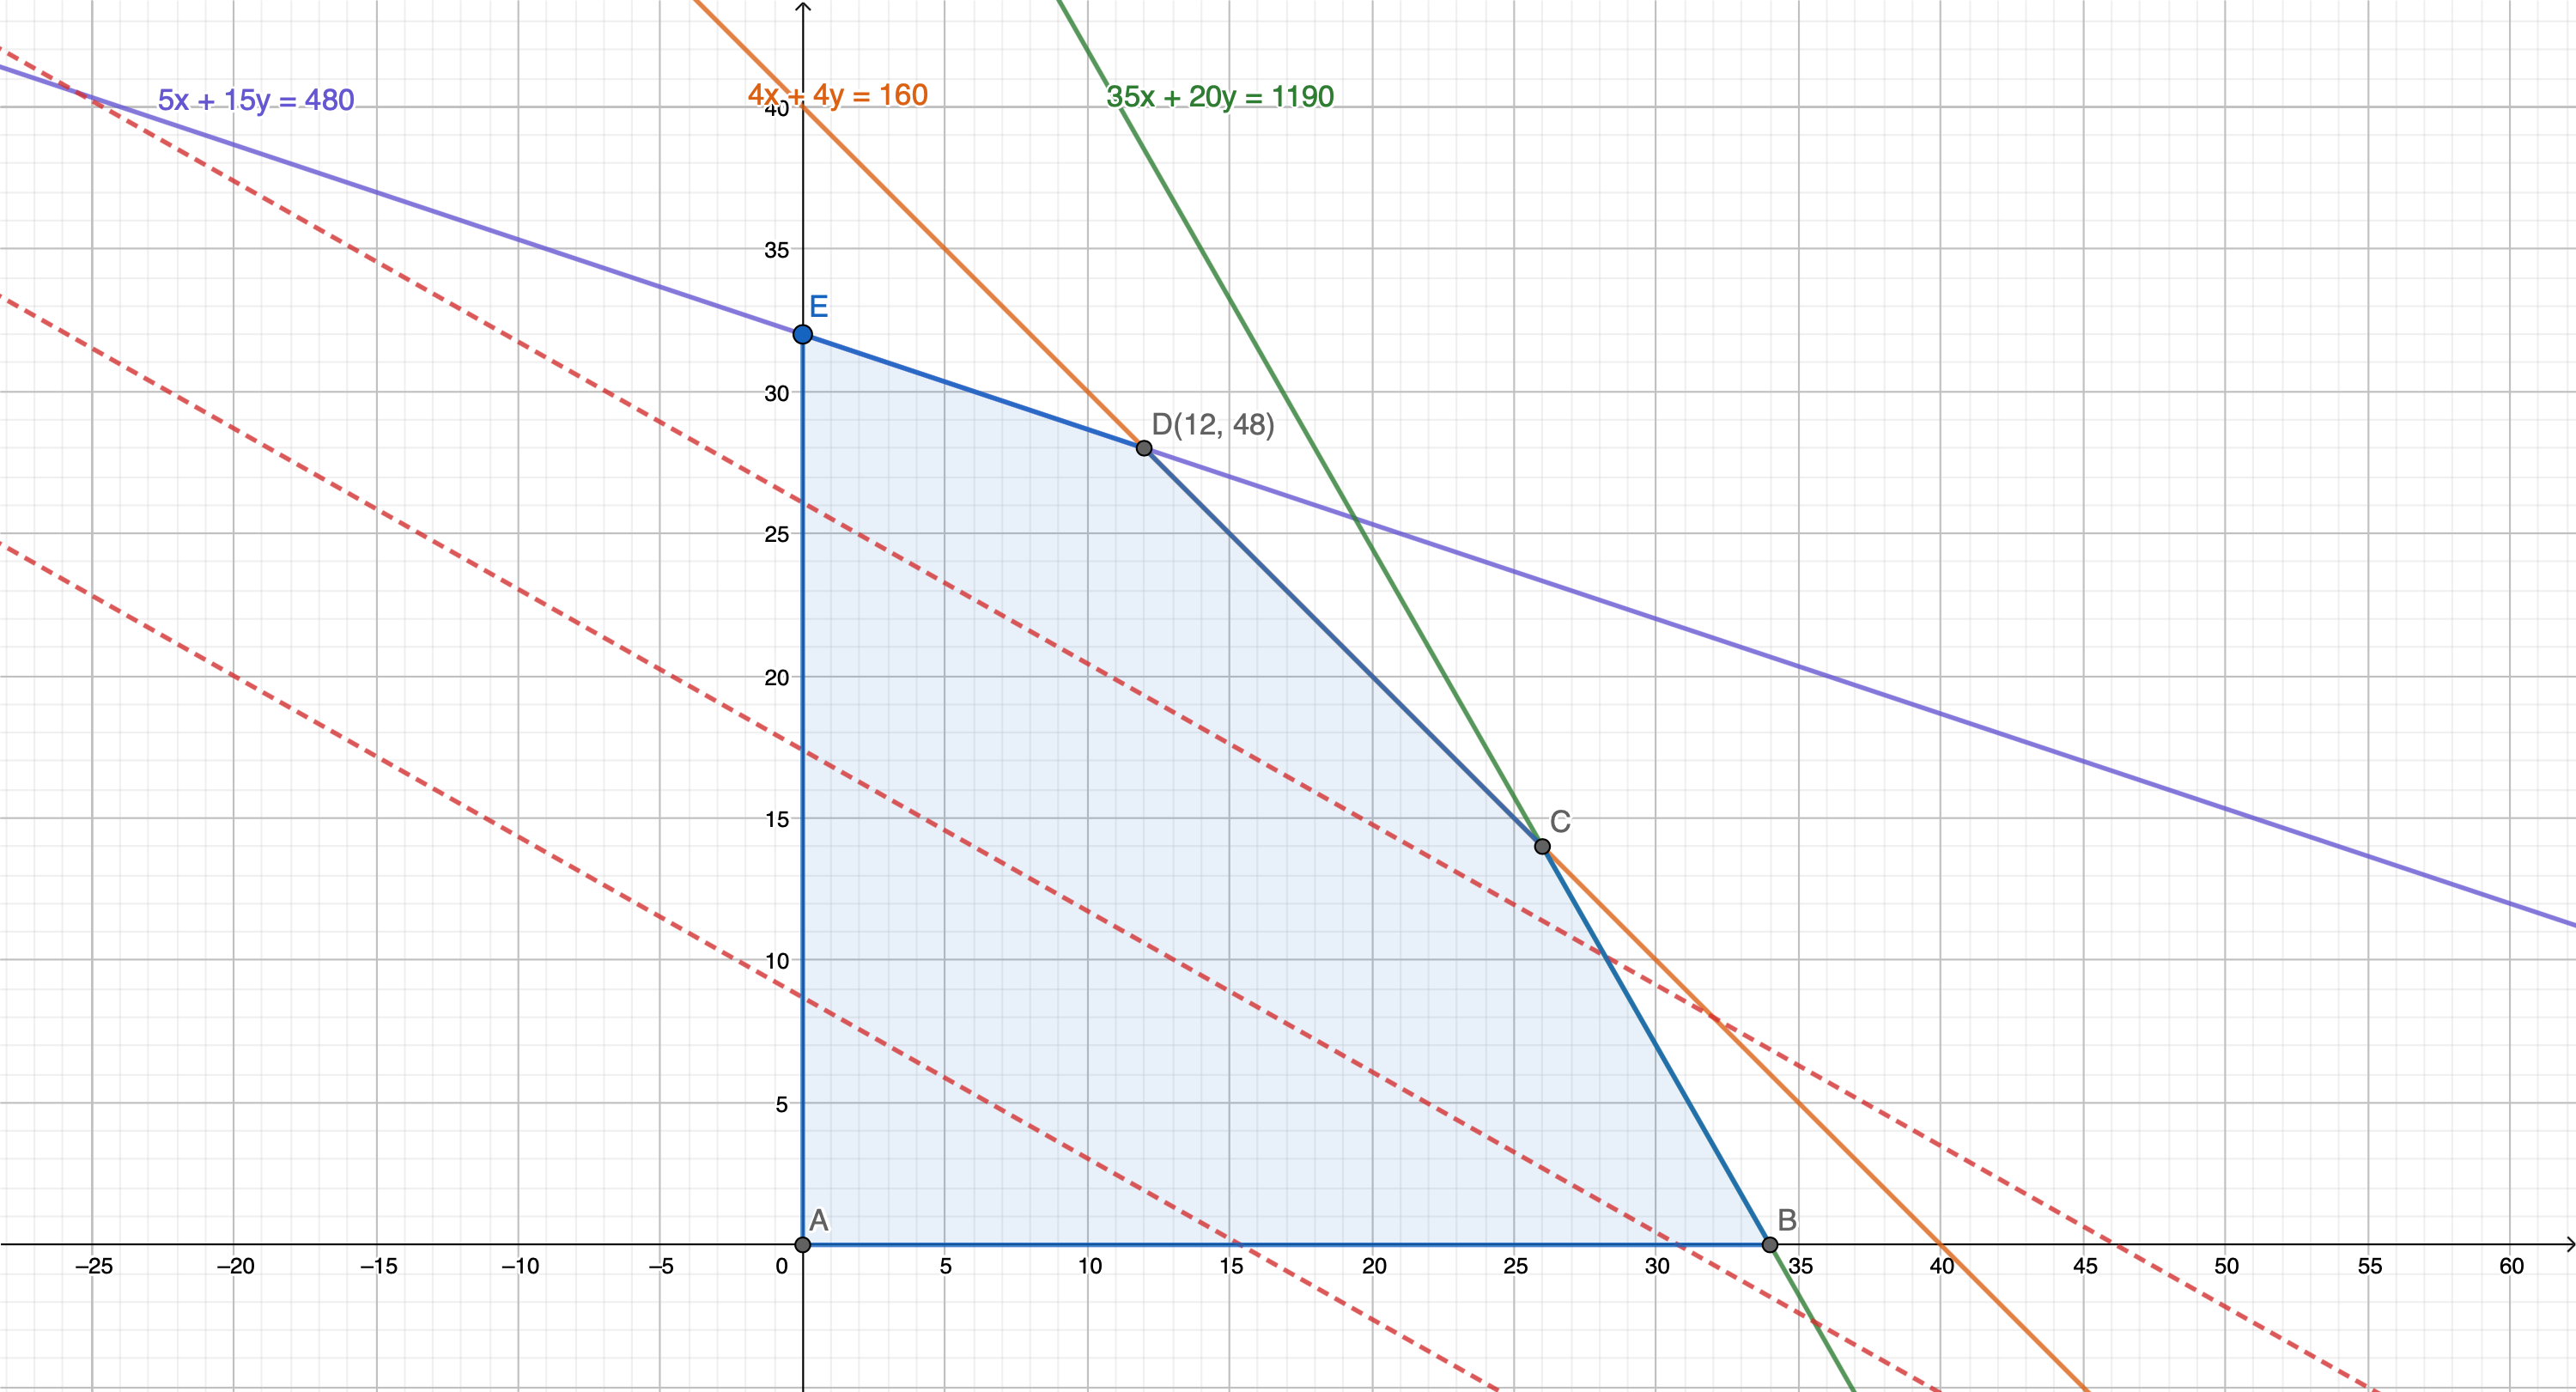
\includegraphics[width=0.75\linewidth]{image2}
		\vspace{4pt}
		\caption{Linear programming of the brewery profit}
		\label{coordinate2}
	\end{figure}

	\pagebreak
	\textbf{Subproblem b)}
	
	With the consideration of time constraints, we should add the constraints as follow
	\begin{equation}
		1.5x+2.5y \le (12)(7) = 84
	\end{equation}
	Then we solve the optimization problem by drawing the linear programming graph as Figure \ref{coordinate3}. As we can see from Figure \ref{coordinate3}, the red dash line is the profit function with variable profits. And the points in the blue area are the available decisions, and the pink line is the new adding time constraint. So we can find the maximum of profit with the point $ E(x=6, y=30) $ as
	\begin{equation}
		f(x,y)_{max} = 130x+230y= (130)(6)+(230)(30)=7680
	\end{equation}
	\vspace{-20pt}
		\begin{figure}[htbp]
		\centering
		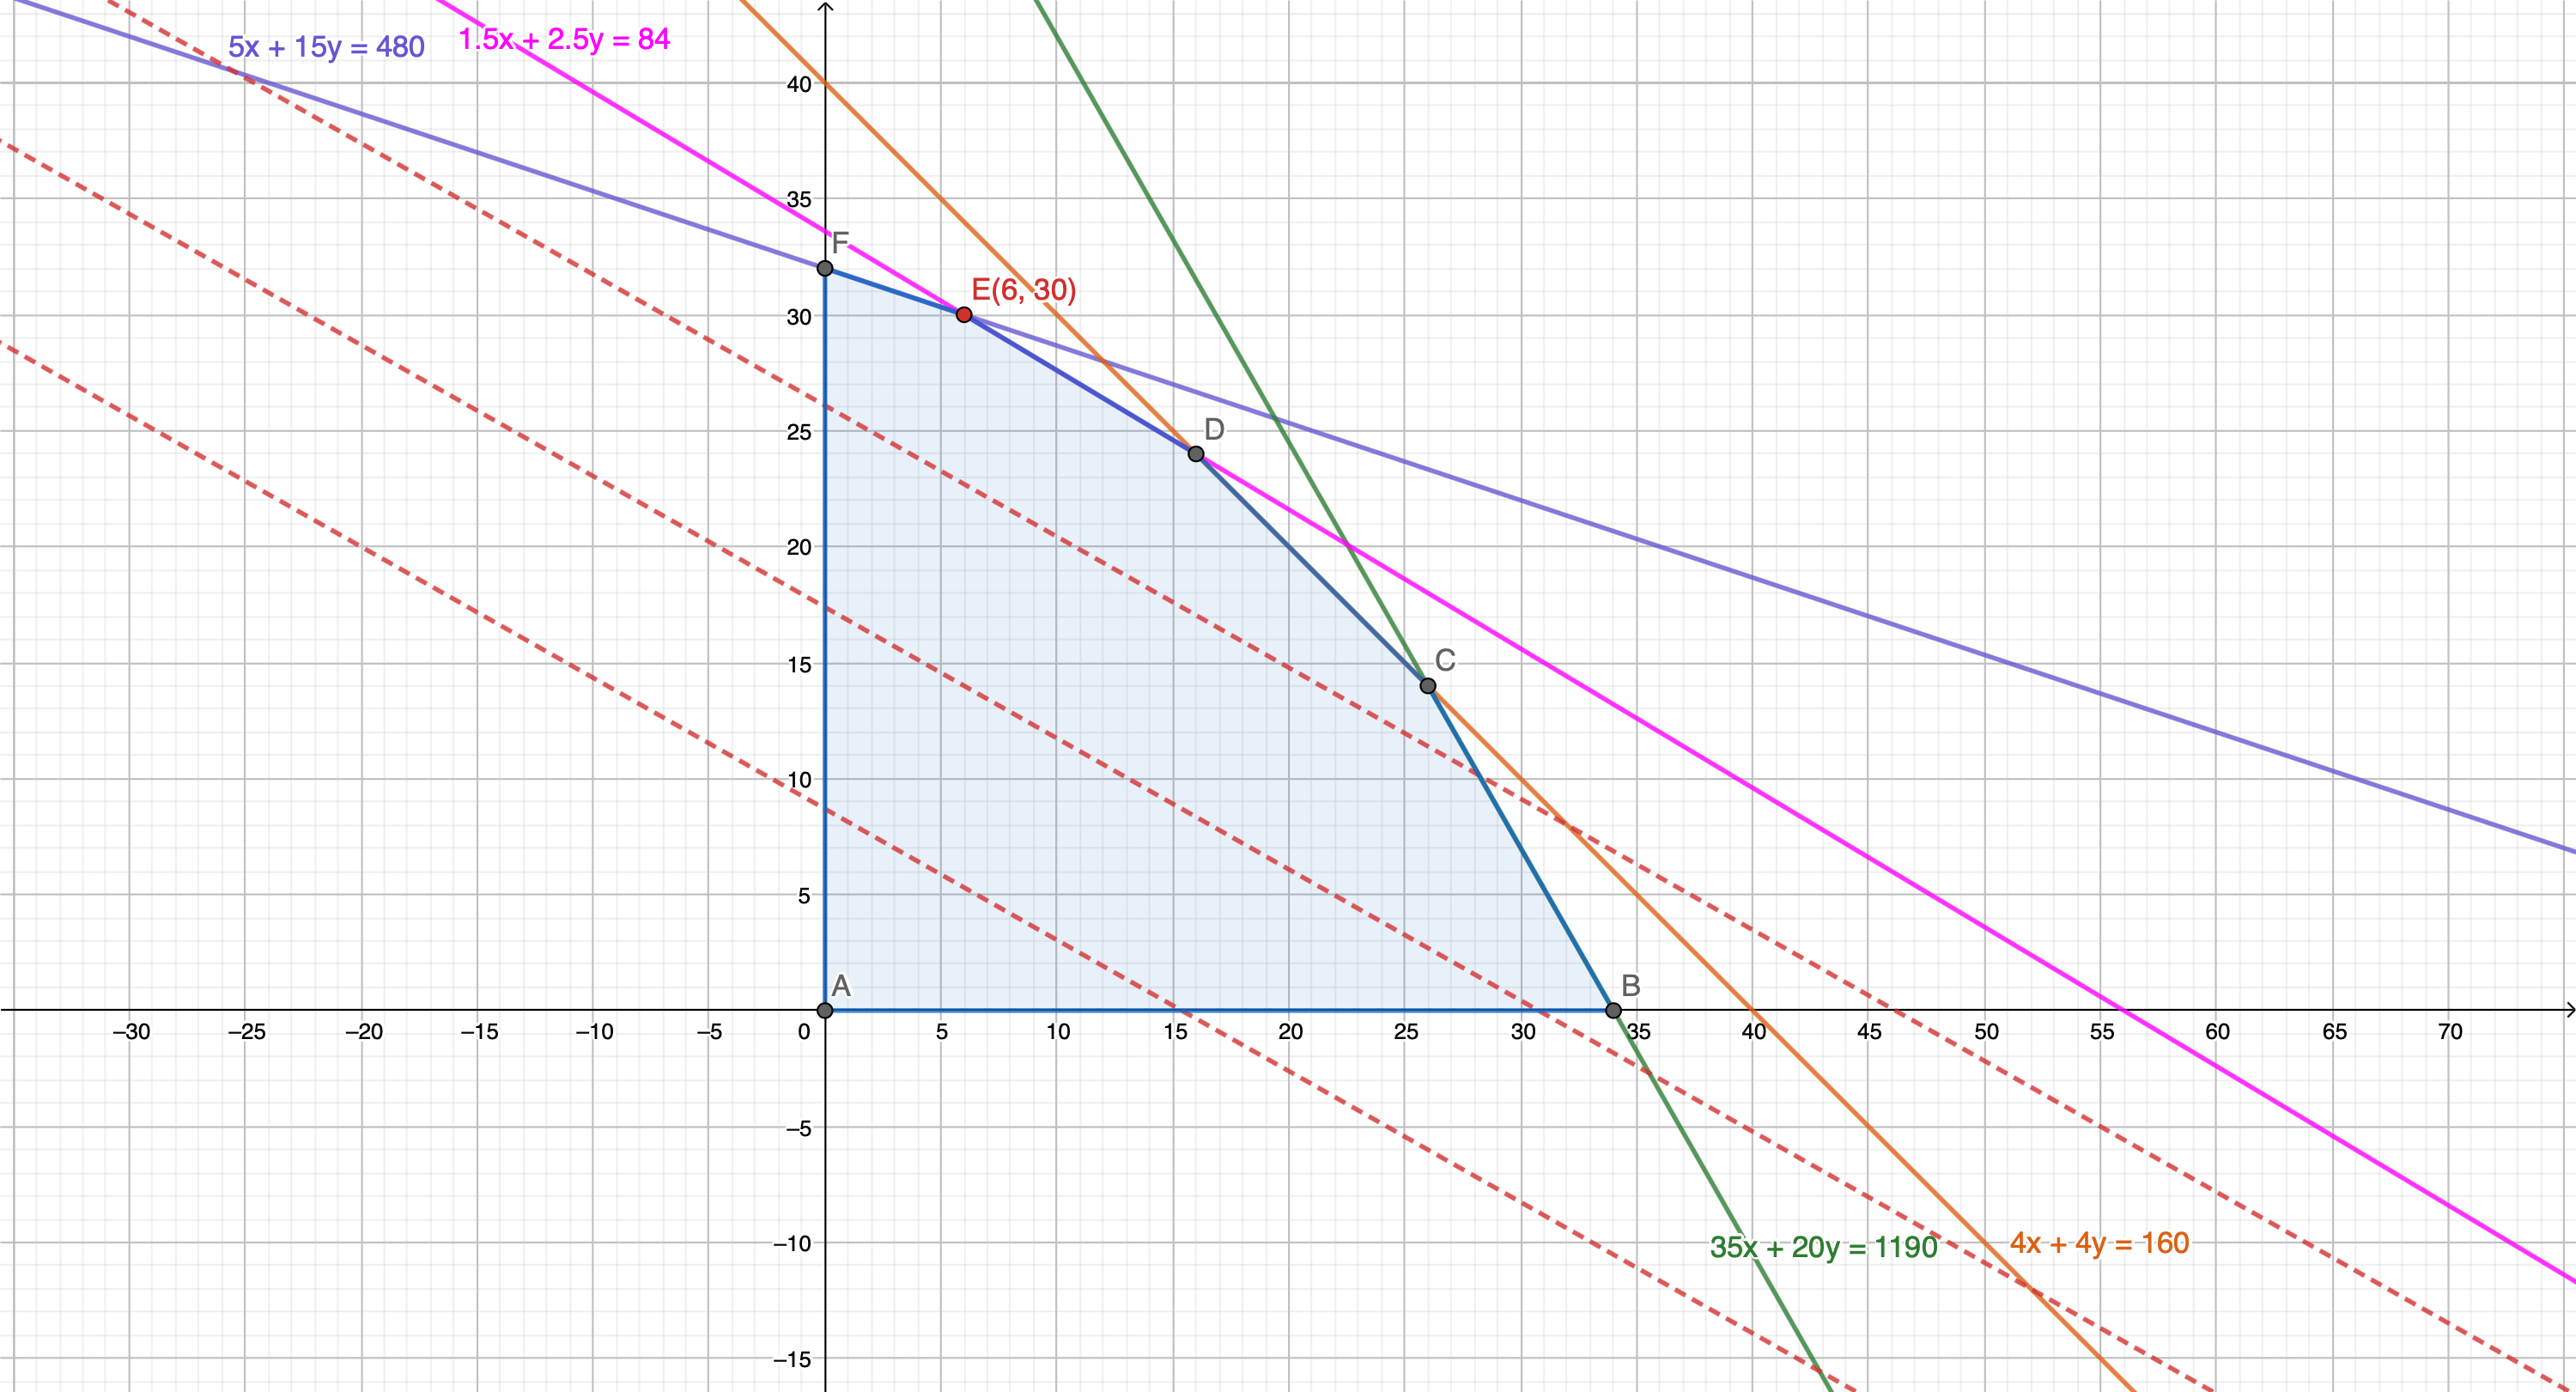
\includegraphics[width=0.75\linewidth]{image3}
		\vspace{4pt}
		\caption{Linear programming with time constraint}
		\label{coordinate3}
	\end{figure}
\end{homeworkProblem}
\vspace{-20pt}
\begin{homeworkProblem}
	Classify the following matrices and verify whether they are positive definite, positive semidefinite or indefinite.
	
	\begin{align*}
		A_1 =
		\begin{pmatrix} 
			1 & 0 & 0 \\ 
			0 & 2 & 0 \\
			0 & 0 & -1 \\
		\end{pmatrix},\quad
		A_2 =
		\begin{pmatrix} 
			1 & 0 & 1 \\ 
			0 & 1 & 2 \\
			1 & 2 & 5 \\
		\end{pmatrix},\quad
		A_3 =
			\begin{pmatrix} 
			1 & 0 & 1 \\ 
			0 & 1 & -1 \\
			0 & 2 & 4 \\
		\end{pmatrix},\quad
		A_4 =
		\begin{pmatrix} 
		1 & 0 & 1 \\ 
		0 & -1 & -1 \\
		-1 & 1 & 0 \\
		\end{pmatrix}.
	\end{align*}
	
	What are the eigenvalues of the matrices \(A_3\) and \(A_4\)?
	
	\vspace{4pt}
	\textbf{\large{Solution}}
	
	$\circ$ \textbf{For matrix \(A_1\):} Because matrix \(A_1\) is a diagonal matrix, we can get the eigenvalues of \(A_1\) as $\lambda_1=1,\lambda_2=2,\lambda_3=-1$. Thus, two eigenvalues are positive, and one eigenvalue is negative, so matrix \(A_1\) is \textbf{indefinite}.
	
	\vspace{4pt}
	$\circ$ \textbf{For matrix \(A_2\):} Because matrix \(A_2\) is a real symmetric matrix, we can use the eigenvalues of \(A_2\) to judge the definiteness of matrix \(A_2\).
	
	The characteristic polynomial of \(A_2\) can be derived as follow
	\begin{equation}
		\begin{split}
			\begin{vmatrix}
				A_2-\lambda I
			\end{vmatrix}&=
			\begin{vmatrix}
			1-\lambda & 0 & 1 \\ 
			0 & 1-\lambda & 2 \\
			1 & 2 & 5-\lambda 
			\end{vmatrix}\\
			&=(1-\lambda)
			\begin{vmatrix}
				1-\lambda&2\\
				2&5-\lambda
			\end{vmatrix}
			+
			(1)
			\begin{vmatrix}
				0&1-\lambda\\
				1&2
			\end{vmatrix}\\
			&=\lambda(1-\lambda)(\lambda-6)
		\end{split}
	\end{equation}
	Thus, the eigenvalues of \(A_2\) can be derived as $\lambda_1=0,\lambda_2=1,\lambda_3=6$. So $\forall \lambda_i\ge 0$, thus matrix \(A_2\) is \textbf{positive semidefinite}.
	
	$\circ$ \textbf{For matrix \(A_3\):} For $\forall \textbf{\textit{x}}\in \mathbb{R}^3$, we have
	\begin{equation}
		\begin{split}
			\textbf{\textit{x}}^TA_3\textbf{\textit{x}} &=
			\begin{pmatrix}
				x_1 & x_2 & x_3
			\end{pmatrix} 
			\begin{pmatrix}
				1 & 0 & 1 \\ 
				0 & 1 & -1 \\
				0 & 2 & 4 \\
			\end{pmatrix}
			\begin{pmatrix}
				x_1\\
				x_2\\
				x_3\\
			\end{pmatrix}\\
			&=
			\begin{pmatrix}
				x_1 & x_2+2x_3 & x_1-x_2+4x_3
			\end{pmatrix} 
			\begin{pmatrix}
				x_1\\
				x_2\\
				x_3\\
			\end{pmatrix} \\
			&=
			x_1^2+x_2^2+4x_3^2+x_2x_3+x_1x_3\\
			&=\left(x_1+\frac{1}{2}x_3\right)^2+\left(x_2+\frac{1}{2}x_3\right)^2+\frac{7}{2}x_3^2\ge 0
		\end{split}
	\end{equation}
	Thus we can find $\textbf{\textit{x}}^TA_3\textbf{\textit{x}}>0$ for $\forall \textbf{\textit{x}}\in\mathbb{R}^3\backslash \left\{\textbf{0}\right\}$. So matrix \(A_3\) is \textbf{positive definite}.
	
	\vspace{4pt}
	In order to calculate the eigenvalues of matrix \(A_3\). We write down the characteristic polynomial of \(A_3\) as follow
	\begin{equation}
		\begin{split}
			\begin{vmatrix}
				A_3-\lambda I
			\end{vmatrix}&=
			\begin{vmatrix}
				1-\lambda & 0 & 1 \\ 
				0 & 1-\lambda & -1 \\
				0 & 2 & 4-\lambda 
			\end{vmatrix}\\
			&=(1-\lambda)
			\begin{vmatrix}
				1-\lambda&-1\\
				2&4-\lambda
			\end{vmatrix}\\
			&=(1-\lambda)(\lambda-2)(\lambda-3)
		\end{split}
	\end{equation}
	Thus, the eigenvalues of \(A_3\) can be derived as $\lambda_1=1,\lambda_2=2,\lambda_3=3$.
	
	$\circ$ \textbf{For matrix \(A_4\):} For $\forall \textbf{\textit{x}}\in \mathbb{R}^3$, we have
	\begin{equation}
		\begin{split}
			\textbf{\textit{x}}^TA_4\textbf{\textit{x}} &=
			\begin{pmatrix}
				x_1 & x_2 & x_3
			\end{pmatrix} 
			\begin{pmatrix}
				1 & 0 & 1 \\ 
				0 & -1 & -1 \\
				-1 & 1 & 0 \\
			\end{pmatrix}
			\begin{pmatrix}
				x_1\\
				x_2\\
				x_3\\
			\end{pmatrix}\\
			&=
			\begin{pmatrix}
				x_1-x_3 & -x_2+x_3 & x_1-x_2
			\end{pmatrix} 
			\begin{pmatrix}
				x_1\\
				x_2\\
				x_3\\
			\end{pmatrix} \\
			&=
			x_1^2-x_2^2\\
		\end{split}
	\end{equation}
	So when $x_1\ge x_2, \textbf{\textit{x}}^TA_4\textbf{\textit{x}}\ge 0$; when $x_1\le x_2, \textbf{\textit{x}}^TA_4\textbf{\textit{x}} \le0$. Thus matrix \(A_4\) is \textbf{indefinite}.
	
	\vspace{4pt}
	In order to calculate the eigenvalues of matrix \(A_4\). We write down the characteristic polynomial of \(A_4\) as follow
	\begin{equation}
		\begin{split}
			\begin{vmatrix}
				A_4-\lambda I
			\end{vmatrix}&=
			\begin{vmatrix}
				1-\lambda & 0 & 1 \\ 
				0 & -1-\lambda & -1 \\
				-1 & 1 & -\lambda 
			\end{vmatrix}\\
			&=(1-\lambda)
			\begin{vmatrix}
				-1-\lambda&-1\\
				1&-\lambda
			\end{vmatrix}
			+(1)
			\begin{vmatrix}
				0 & -1-\lambda\\
				-1 & 1
			\end{vmatrix}
			\\
			&=-\lambda(\lambda^2+1)
		\end{split}
	\end{equation}
	Thus, the eigenvalues of \(A_4\) can be derived as $\lambda_1=0,\lambda_2=i,\lambda_3=-i$.
\end{homeworkProblem}
\begin{homeworkProblem}
	Let \(y^1,y^2,\dots,y^k\) be $ k $ different and given points in \(\mathbb{R}^2\), i.e., it holds that \(y^i \in \mathbb{R}^2\) for all \(i=1,\dots,k\). We want to find a circle in \(\mathbb{R}^2\) with minimum radius that contains all of these points.
	
	\vspace{4pt}
	Formulate this problem as an optimization problem with the center and radius of the circle as optimization variables. Classify this type of optimization problem.
	
	\vspace{4pt}
	\textbf{\large{Solution}}
	
	We set the center of the circle as $\textbf{\textit{x}}\in\mathbb{R}^2$, and the radius of the circle as $r\in\mathbb{R}$. Thus we can get the follow definition of the optimization problem.
	
	\vspace{4pt}
	$\circ$ \textbf{Decisions variable:} the center of the circle \textbf{\textit{x}}, and the radius of the circle \(r\). 
	
	$\circ$ \textbf{Objective:} minimize the ridus \(r\).
	
	$\circ$ \textbf{Constraints:} The circle should contains all the given points \(y^1,y^2,\dots,y^k\):
	\begin{equation}
		\forall i=1,\dots,k,\quad\left\|y^i-\textbf{\textit{x}}\right\| \le r
	\end{equation}
	
	Thus, the optimization problem can be classified as constrained, nonlinear, continuous optimization problem.
\end{homeworkProblem}
\vspace{-20pt}
\begin{homeworkProblem}
	In this exercise, we want to study and visualize different feasible sets and solve optimization problems via graphical considerations.
	\begin{enumerate}[\quad a)]
		\item Sketch the following sets in $\mathbb{R}^2$:
		
		$\circ$ $X_1:=\{\textbf{\textit{x}}\in\mathbb{R}^2: \left|x_1\right|-\left |x_2\right|\ge 1\}$.
		
		$\circ$ $X_2:=\{\textbf{\textit{x}}\in\mathbb{R}^2: x_1\le0,(x_1+1)^2+x_2^2\ge1\}$.
		
		$\circ$ $X_3:=\{\textbf{\textit{x}}\in\mathbb{R}^2: (x_1-1)^2+x_2^2\le1, x_1-x_2\le0, x_1+x_2\le0\}$.
		
		$\circ$ $X_4:=\{\textbf{\textit{x}}\in\mathbb{R}^2: x_1x_2\ge0,\left\|\textbf{\textit{x}}\right\|_{\infty}\ge1\}$, where $\left\|\textbf{\textit{x}}\right\|_{\infty}:=\text{max}\{\left|x_1\right|,\left|x_2\right|\}$ denotes the maximum norm in $\mathbb{R}^2$.
		\item Analyze which of the sets $ X_1 $, \(X_2\), $ X_3 $, or $ X_4 $ is bounded and explain your answer.
		\item Consider the nonlinear program
		\begin{equation}
			\label{problem}
			\text{min}\,f(\textbf{\textit{x}})\quad \text{s.t.}\quad \textbf{\textit{x}}\in X_4
		\end{equation}
		and determine (graphically) all local and global minimizer of problem (\ref{problem}) for the two choices $f(\textbf{\textit{x}}):=x_1$ and $f(\textbf{\textit{x}}) :=\frac{1}{2}(x_1^2+x_2^2)$. Are the minimizer strict?
		\item In this part, we consider an optimization problem with equality constraints
		\begin{equation}
			\label{p2}
			\mathop{\min}\limits_{\textbf{\textit{x}}\in\mathbb{R}^2}\,f(\textbf{\textit{x}})=\frac{1}{2}\left\|\textbf{\textit{x}}\right\|^2\quad s.t. \quad 1-x_1^2+x_2=0
		\end{equation}
		Let us define $ h:\mathbb{R}^2\to \mathbb{R}$, $h(\textbf{\textit{x}})=1-x_1^2+x_2$ and let $\{\textbf{\textit{x}}\in\mathbb{R}^2:h(\textbf{\textit{x}})=0\}$ denote the feasible set associated with problem (\ref{p2}).
		\begin{enumerate}[\quad--]
			\item Draw the sets $L_\alpha:=\{\textbf{\textit{x}}\in\mathbb{R}^2:f(\textbf{\textit{x}})=\alpha\}$ for different values of $\alpha$>0 and the feasible set $ X $ and determine the solution $ \textbf{\textit{x}}^* \in X $ of problem (\ref{p2}) graphically.
			
			\textbf{Remark: }The sets $L_\alpha$ are called \textit{contours} or \textit{contour lines} of $ f $.
			\item Modify your sketch and draw the gradients $\nabla f(\textbf{\textit{x}}^*)$and $\nabla h(\textbf{\textit{x}}^*)$(at the point $ \textbf{\textit{x}}^* $). What kind of connection exists between those two vectors?
		\end{enumerate}
		\item Give an example of a function $ f $ that has a strict local minimum but no global minimum.
	\end{enumerate}
	\textbf{\large{Solution}}
	
	\vspace{4pt}
	\textbf{Subproblem a)}
	
	The graph of $ X_1$ is showed as Figure \ref{p5to1}. The blue area is the feasible points of set $ X_1$. The graph of $ X_2$ is showed as Figure \ref{p5to2}. The blue area is the feasible points of set $ X_2$. The graph of $ X_3$ is showed as Figure \ref{p5to3}. red point $A$ is the only feasible points] of set $ X_3$. The graph of $ X_4$ is showed as Figure \ref{p5to4}. The blue area is the feasible points of set $ X_4$.
	\begin{figure}[htbp]
		\centering
		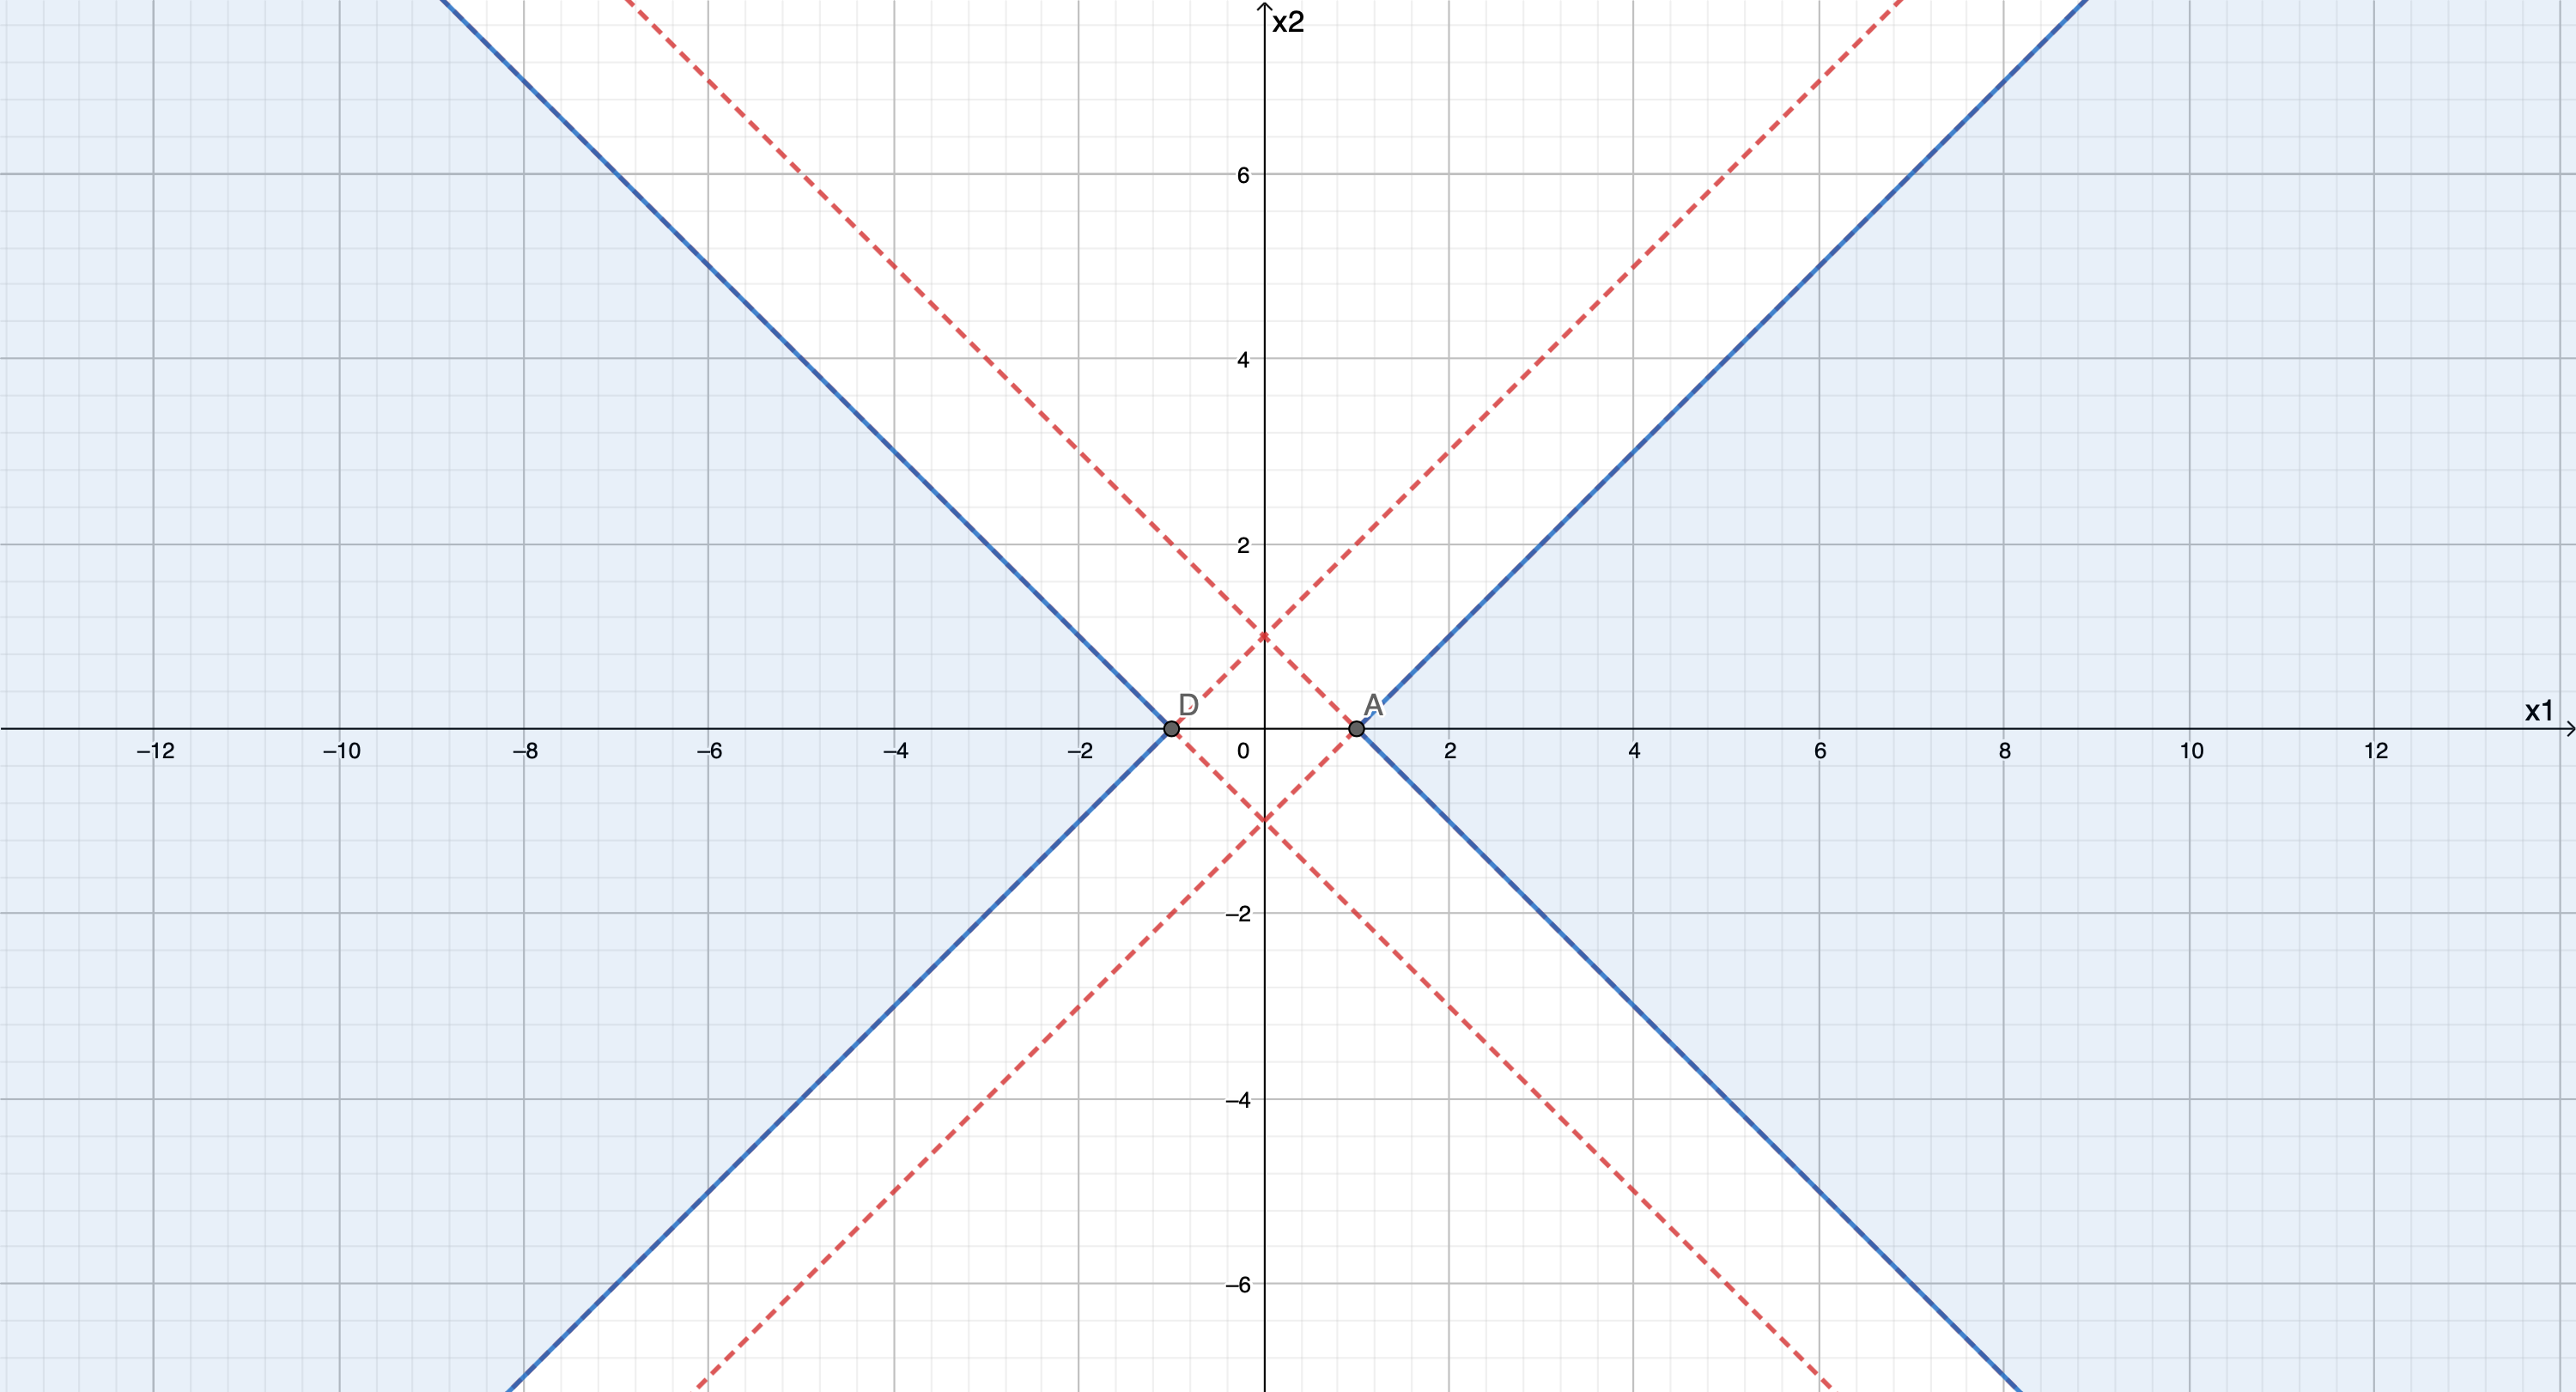
\includegraphics[width=0.8\linewidth]{p5_1}
		\vspace{4pt}
		\caption{Graph of set \textbf{\textit{X}}$ _1 $}
		\label{p5to1}
	\end{figure}
	\begin{figure}[htbp]
		\centering
		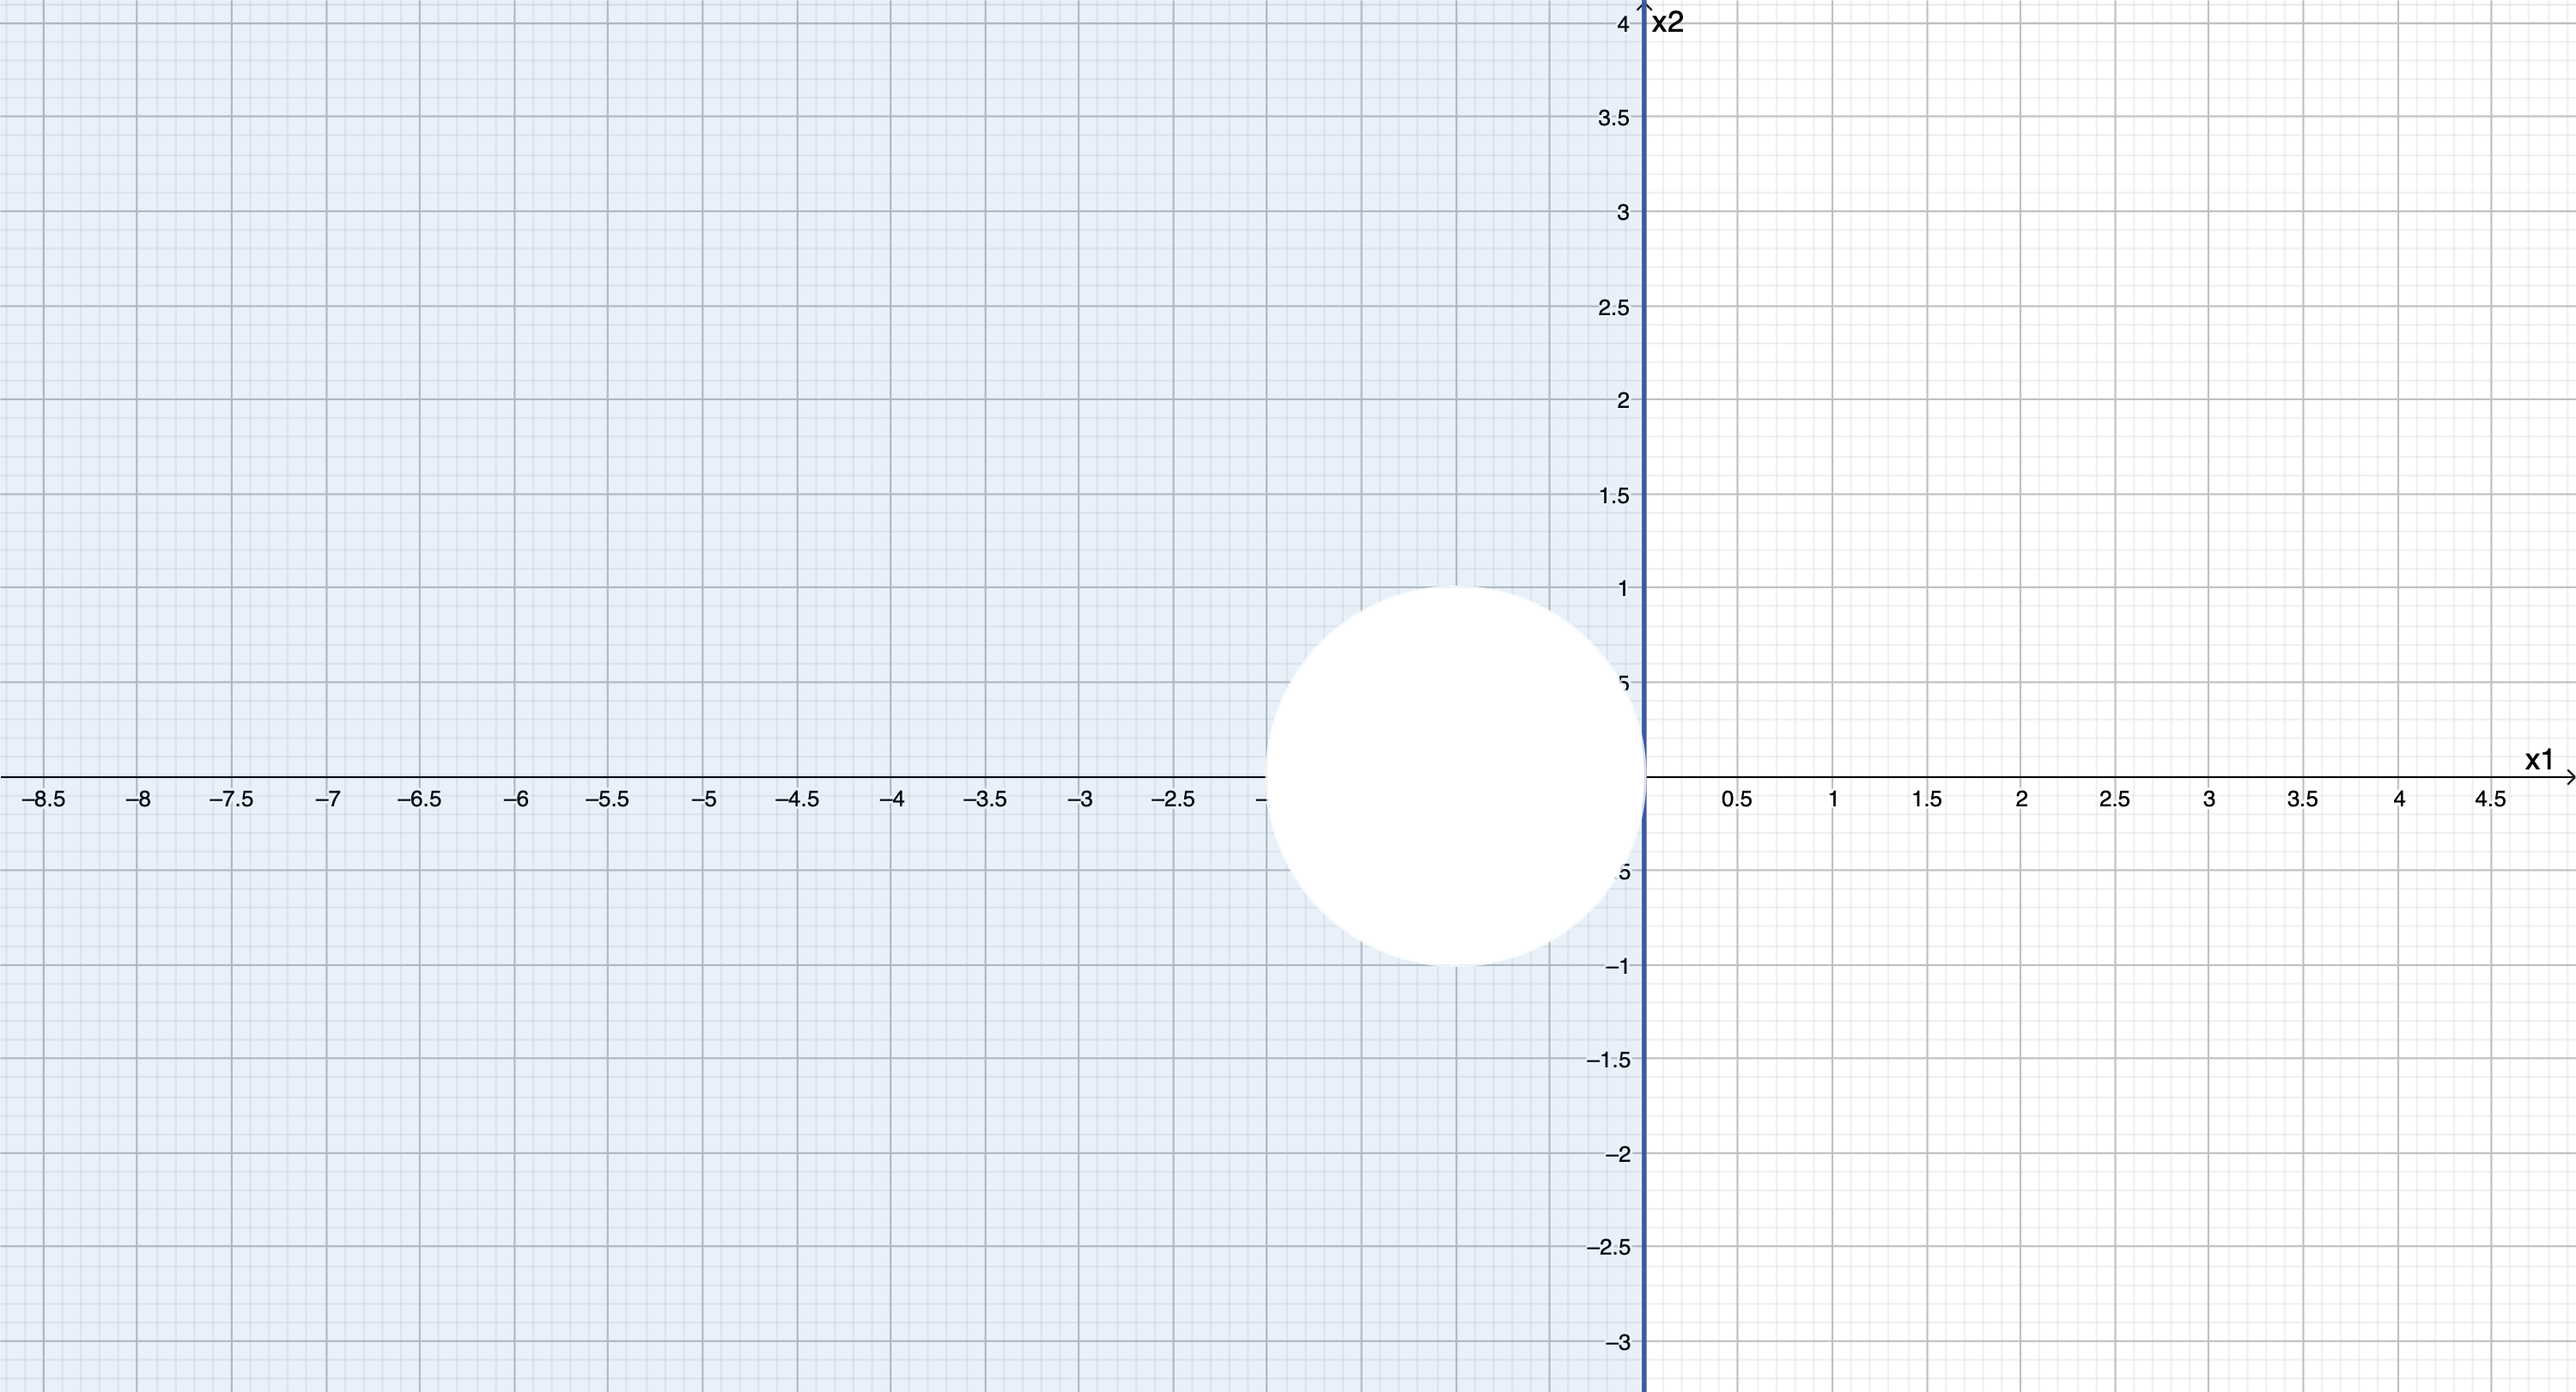
\includegraphics[width=0.8\linewidth]{p5_2}
		\vspace{4pt}
		\caption{Graph of set \textbf{\textit{X}}$ _2 $}
		\label{p5to2}
	\end{figure}
	
	\pagebreak
	\begin{figure}[htbp]
		\centering
		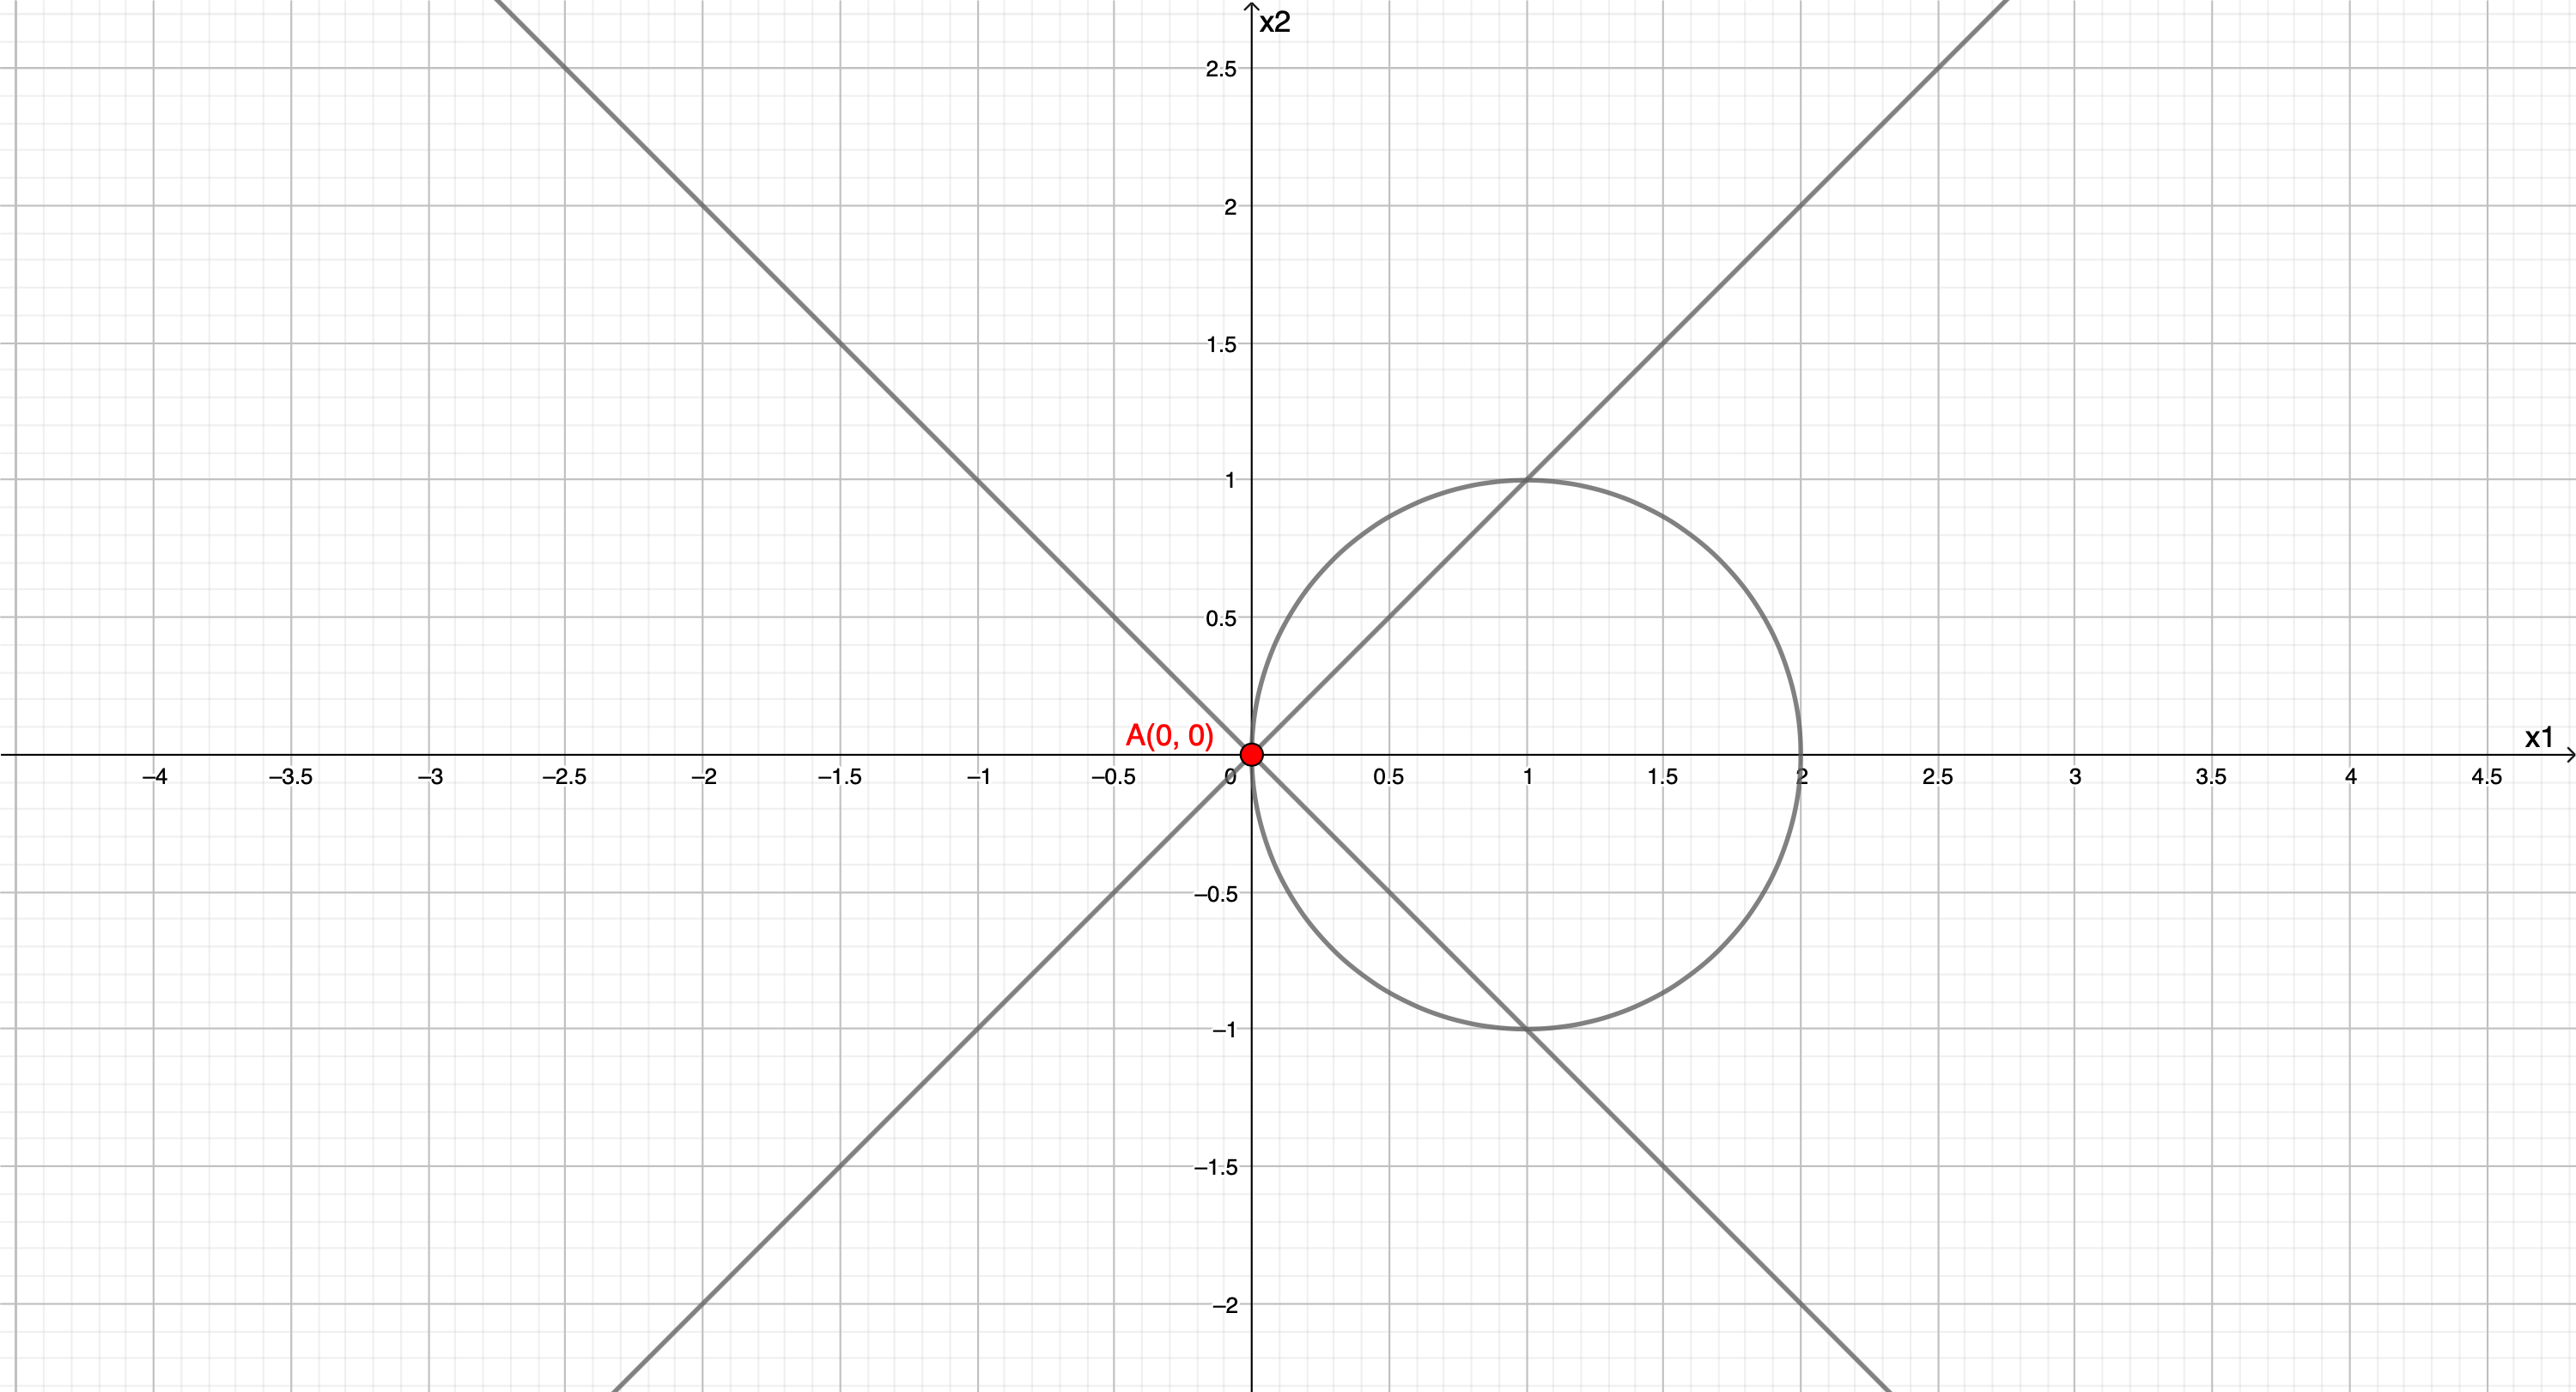
\includegraphics[width=0.7\linewidth]{p5_3}
		\vspace{4pt}
		\caption{Graph of set \textbf{\textit{X}}$ _3 $}
		\label{p5to3}
	\end{figure}
	\begin{figure}[htbp]
		\centering
		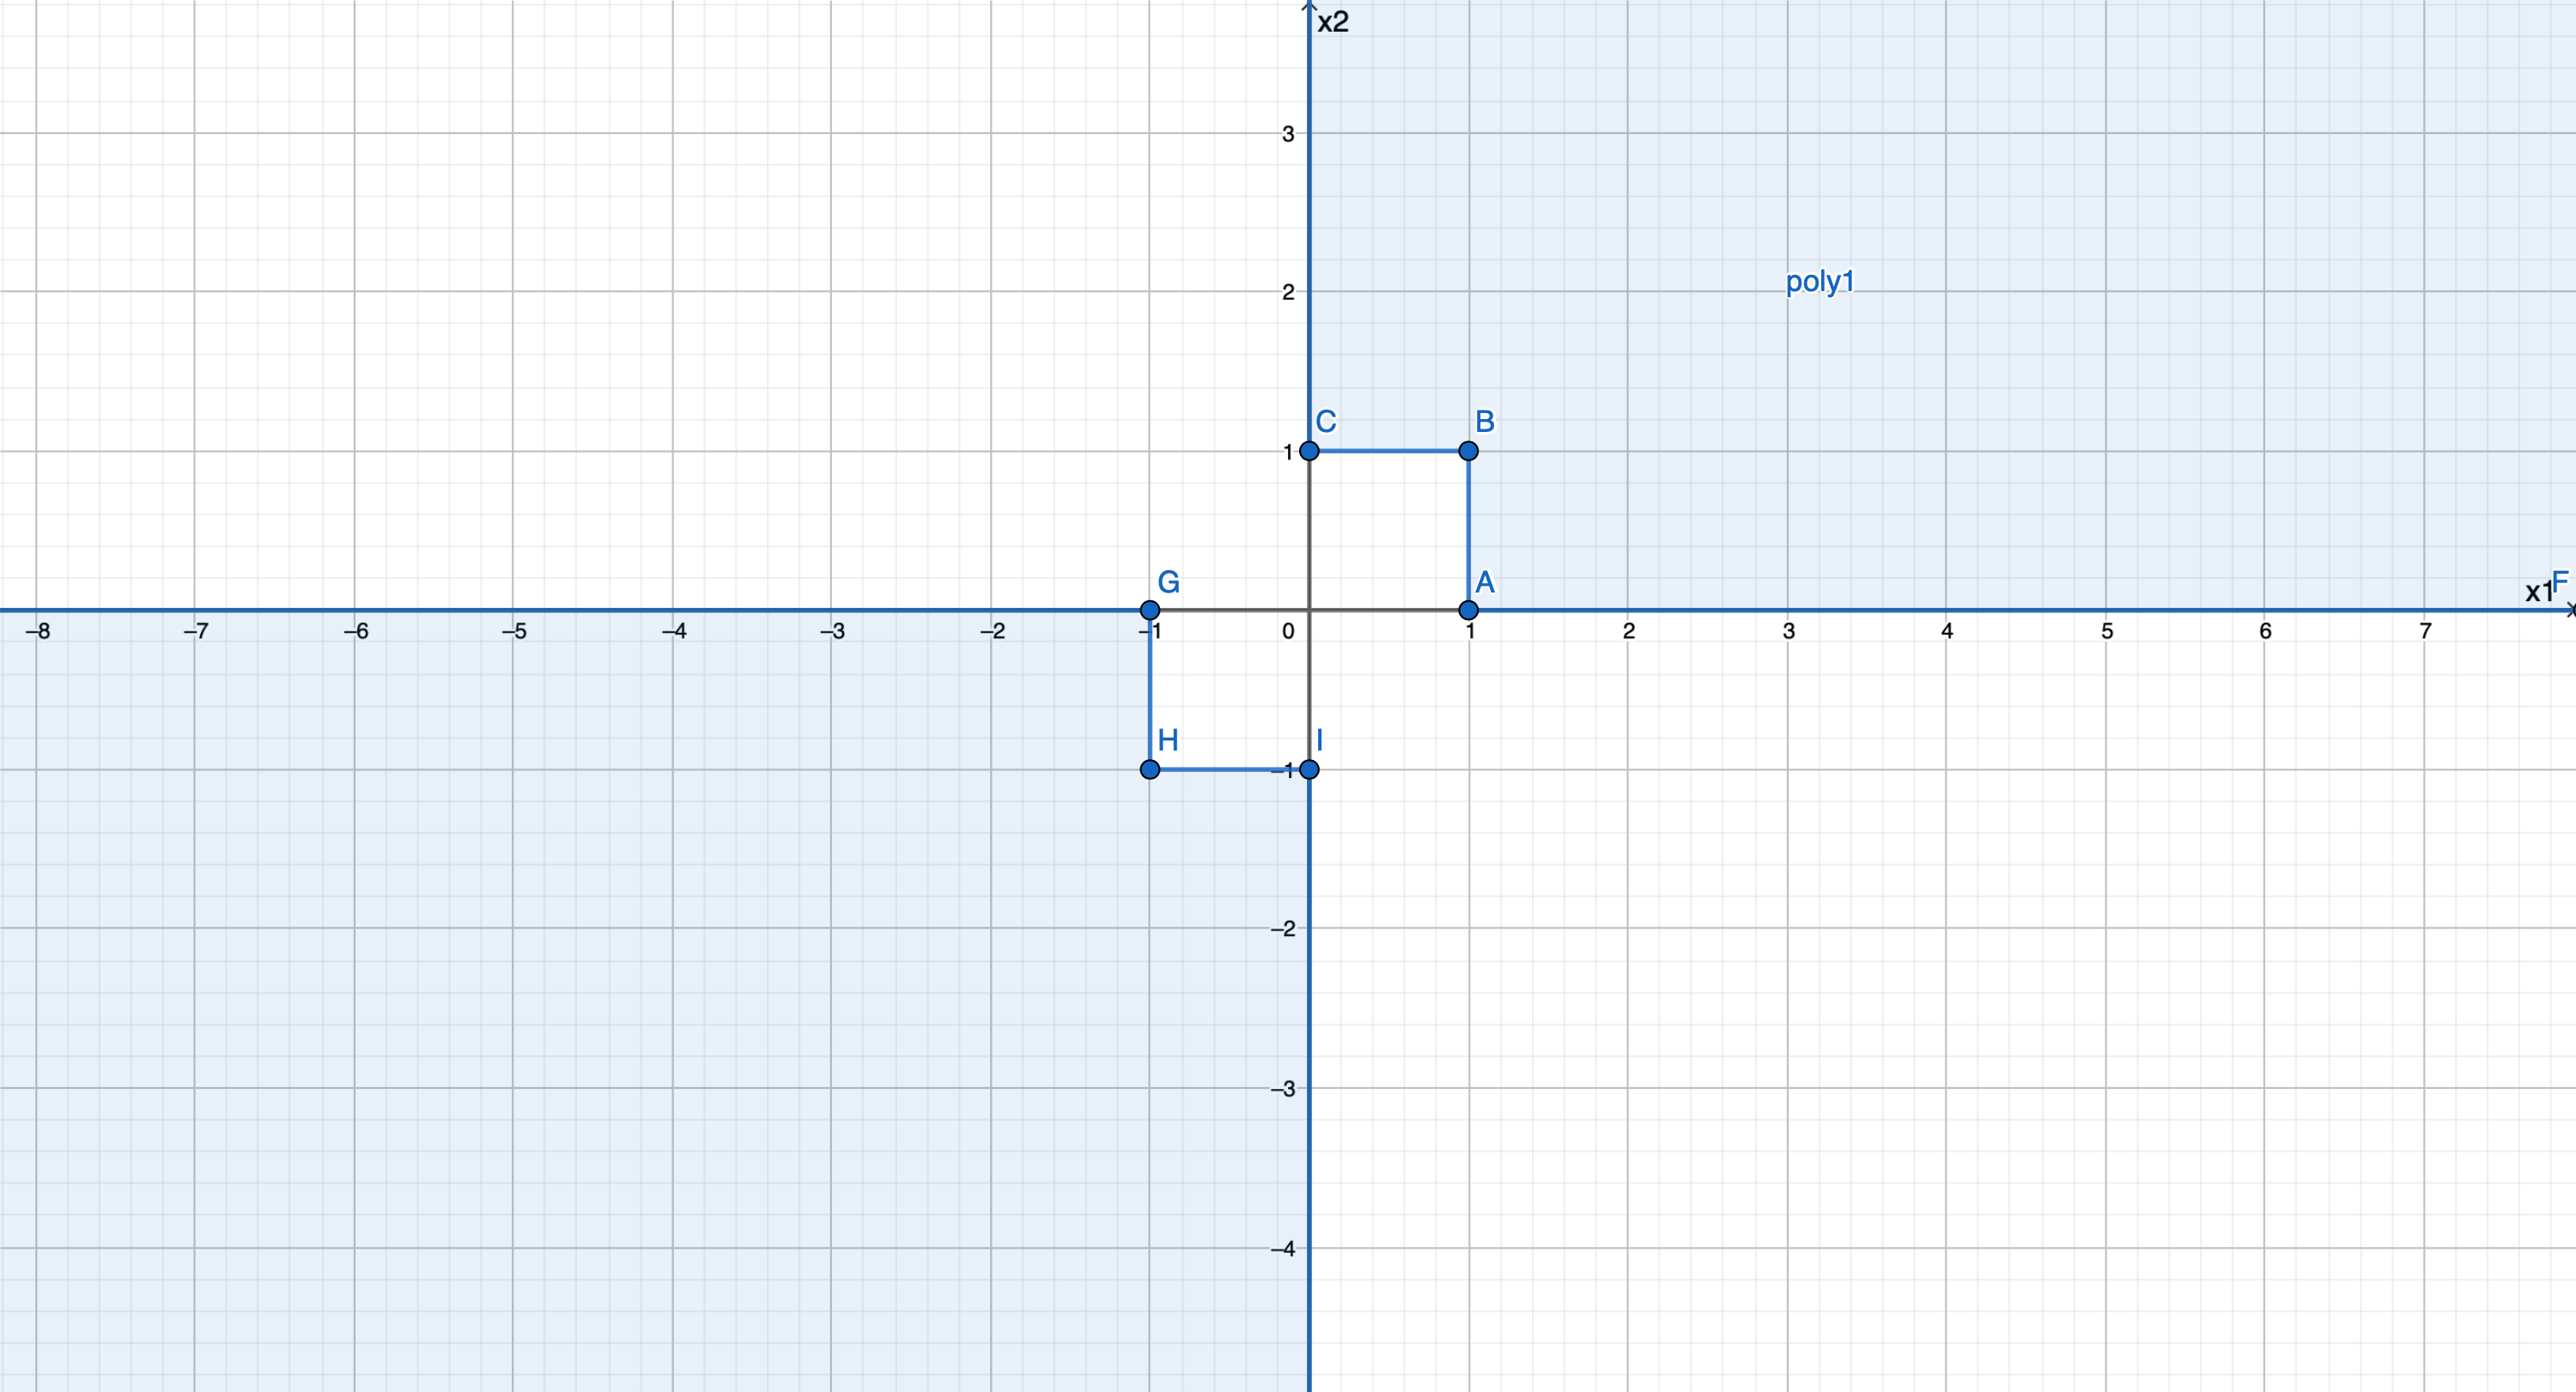
\includegraphics[width=0.7\linewidth]{p5_4}
		\vspace{4pt}
		\caption{Graph of set \textbf{\textit{X}}$ _4 $}
		\label{p5to4}
	\end{figure}

	\vspace{4pt}
	\textbf{Subproblem b)}
	
	$\circ$ Set $X_1$ is not bounded, because both $x_1$ and $x_2$ can reach $\infty$, which means it is not bounded.
	
	$\circ$ Set $X_2$ is not bounded, because $x_1$ can reach $-\infty$ and $x_2$ can reach $\infty$, which means it is not bounded.
	
	$\circ$ Set $X_3$ is bounded, because $x_1$ can only be 0 and $x_2$ can only be 0, which means there is just one point in Set $X_3$, say \textbf{\textit{x}}(0, 0). So Set $X_3$ is bounded.
	
	$\circ$ Set $X_4$ is not bounded, because $x_1$ and $x_2$ can reach $\infty$, which means it is not bounded.
	
	\vspace{4pt}
	\textbf{Subproblem c)}
	
	$\circ$ For the first choice, $f(\textbf{\textit{x}}):=x_1$. Because the variable $x_1$ can can reach all the real number continuously, $ f(x) $ is not bounded (see Figure \ref{p5to5}), which means there is not any local or global minimizer.
	\begin{figure}[htbp]
		\centering
		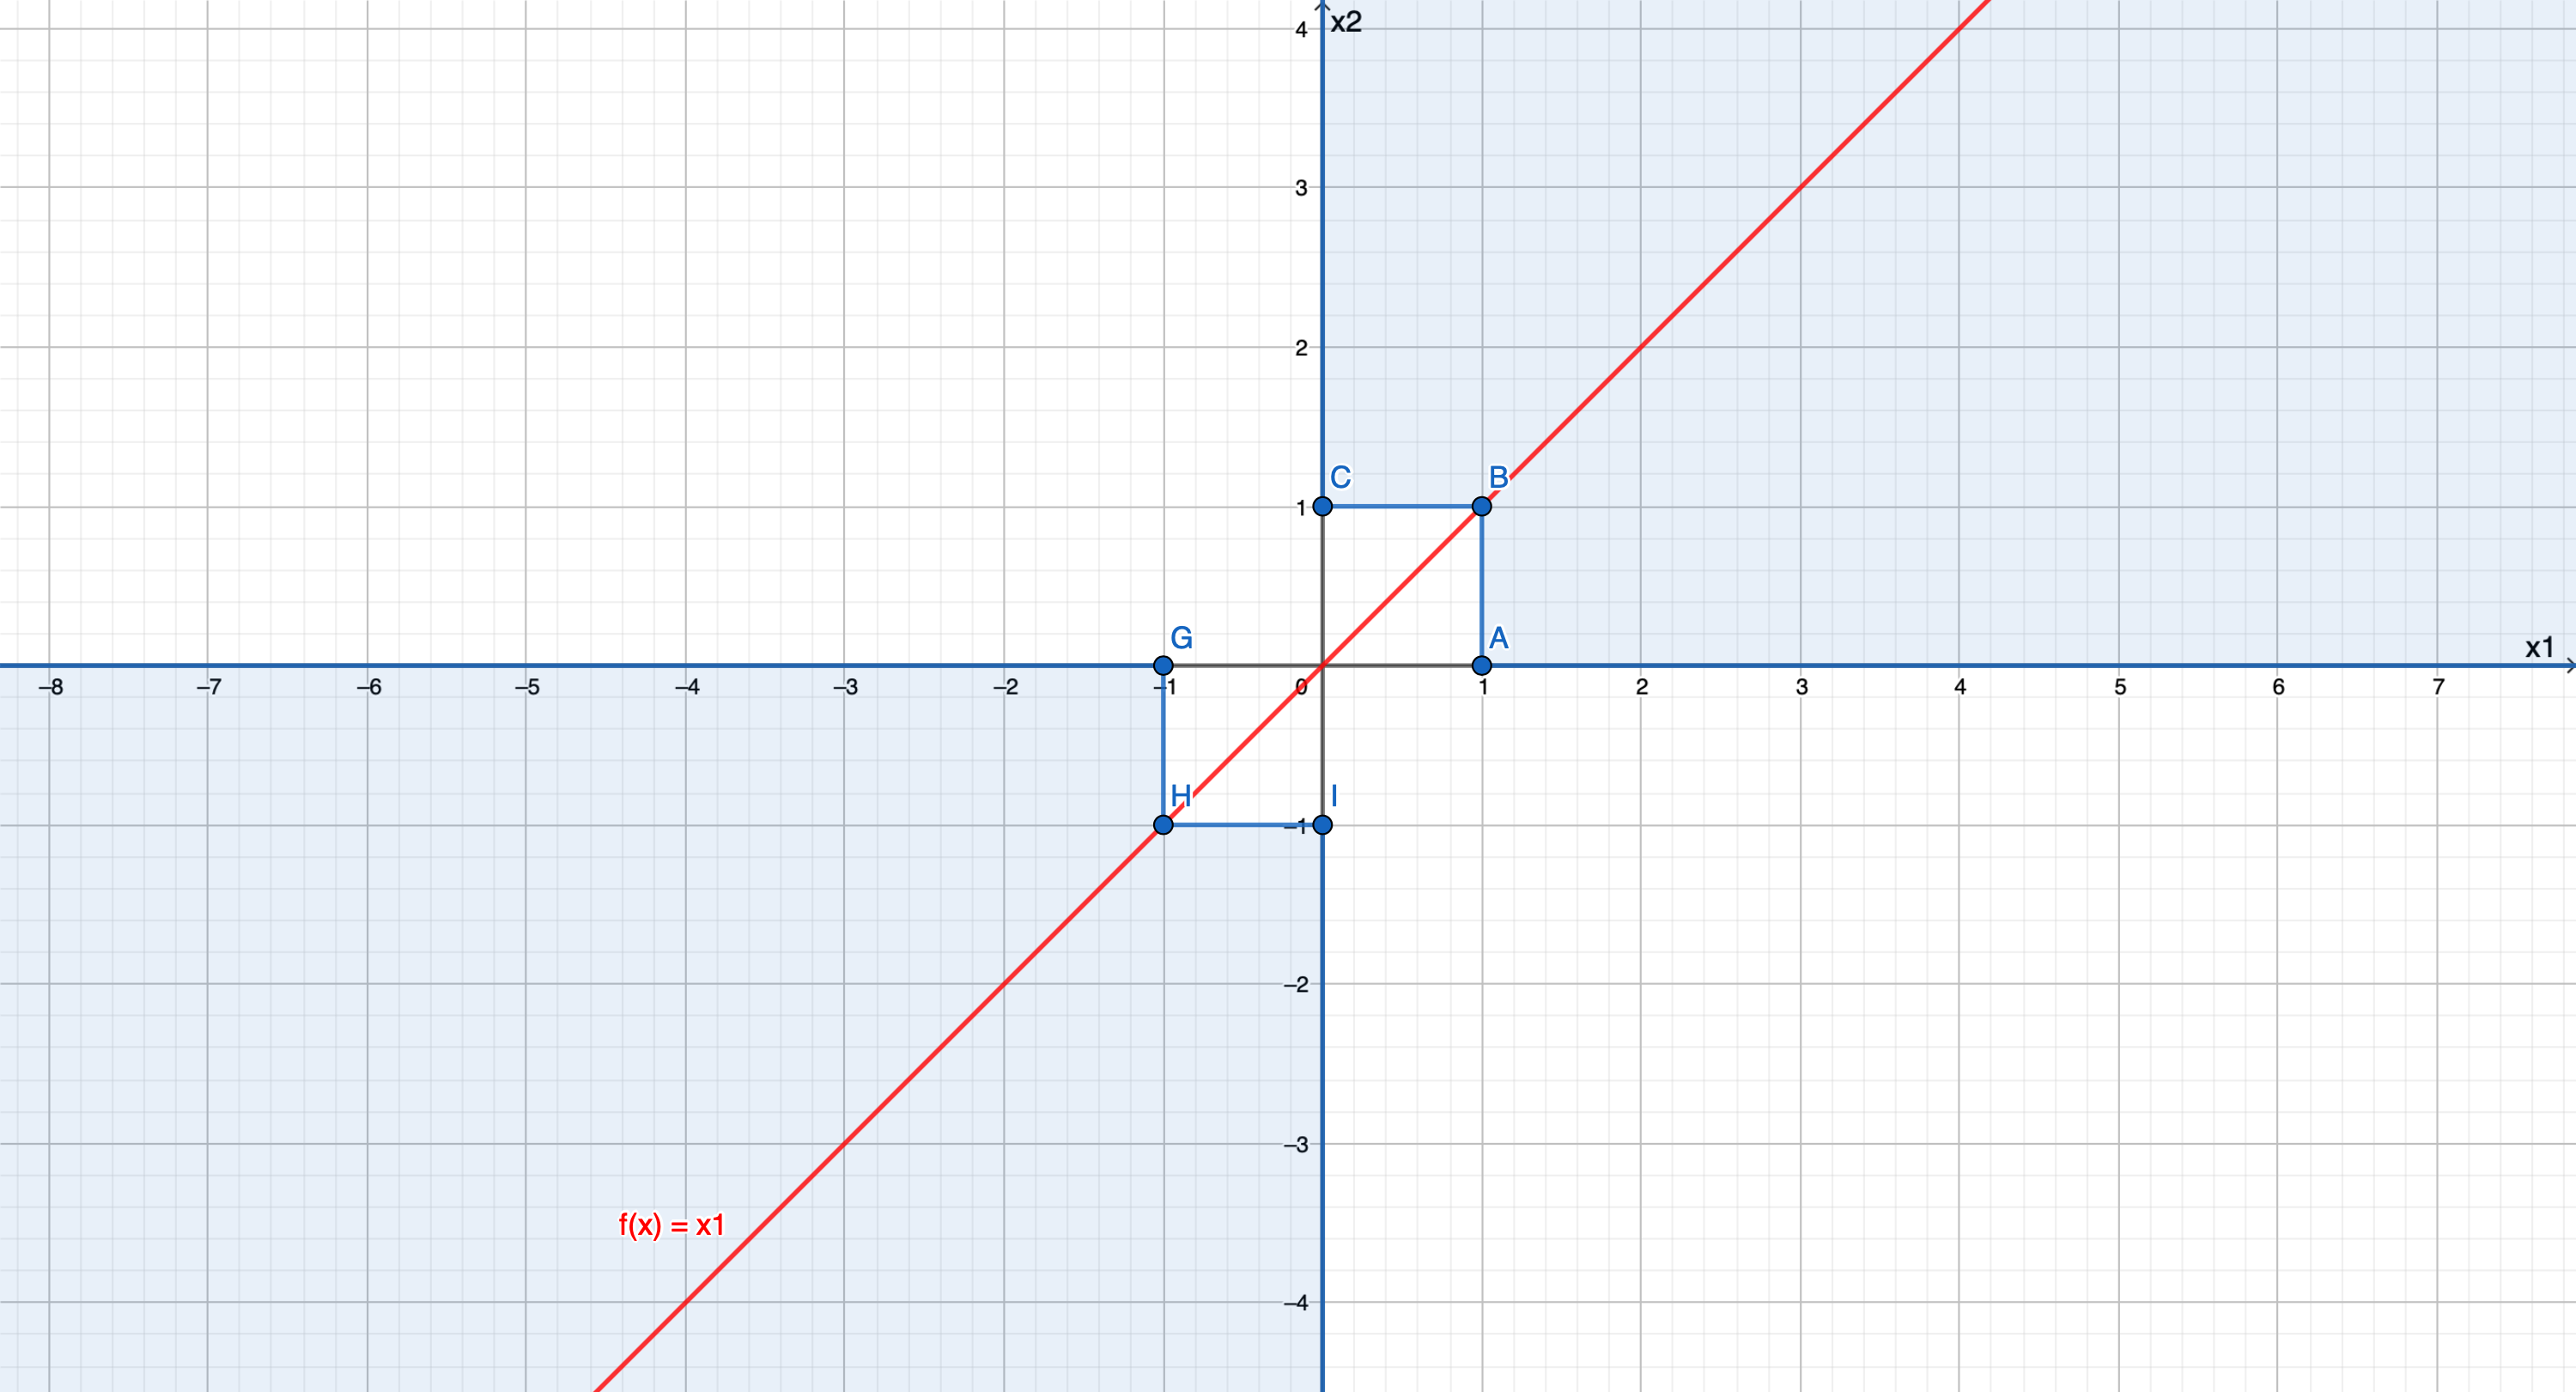
\includegraphics[width=0.55\linewidth]{p5_5}
		\vspace{4pt}
		\caption{$f(\textbf{\textit{x}}) = x_1$}
		\label{p5to5}
	\end{figure}
	
	\vspace{4pt}
	$\circ$ For the second choice, $f(\textbf{\textit{x}}) :=\frac{1}{2}(x_1^2+x_2^2)$. Every time, we can set $ f(\textbf{\textit{x}}) $ as a constant, so we can draw the circle due to the equation. With the constant change, we can get different circles, the circle with the mimimum radius is what we want to find. As we can see in Figure \ref{p5to6}, the red dash circle is drawed according to the eqaution, and the mimimum circle is the circle which goes through point $A$, $C$, $G$, $I$, so these points are global minimizer, but they are not strict global minimizer. However, they are strict local minimizer.
	
	\vspace{4pt}
	Thus, we can find four global minimizer $A(x_1=1, x_2=0)$, $C(x_1=0, x_2=1)$, $G(x_1=-1, x_2=0)$, $I(x_1=0, x_2=-1)$. None of them is strict global minimizer, but all of them are strict local minimizer. 
	
	\pagebreak
	\begin{figure}[htbp]
		\centering
		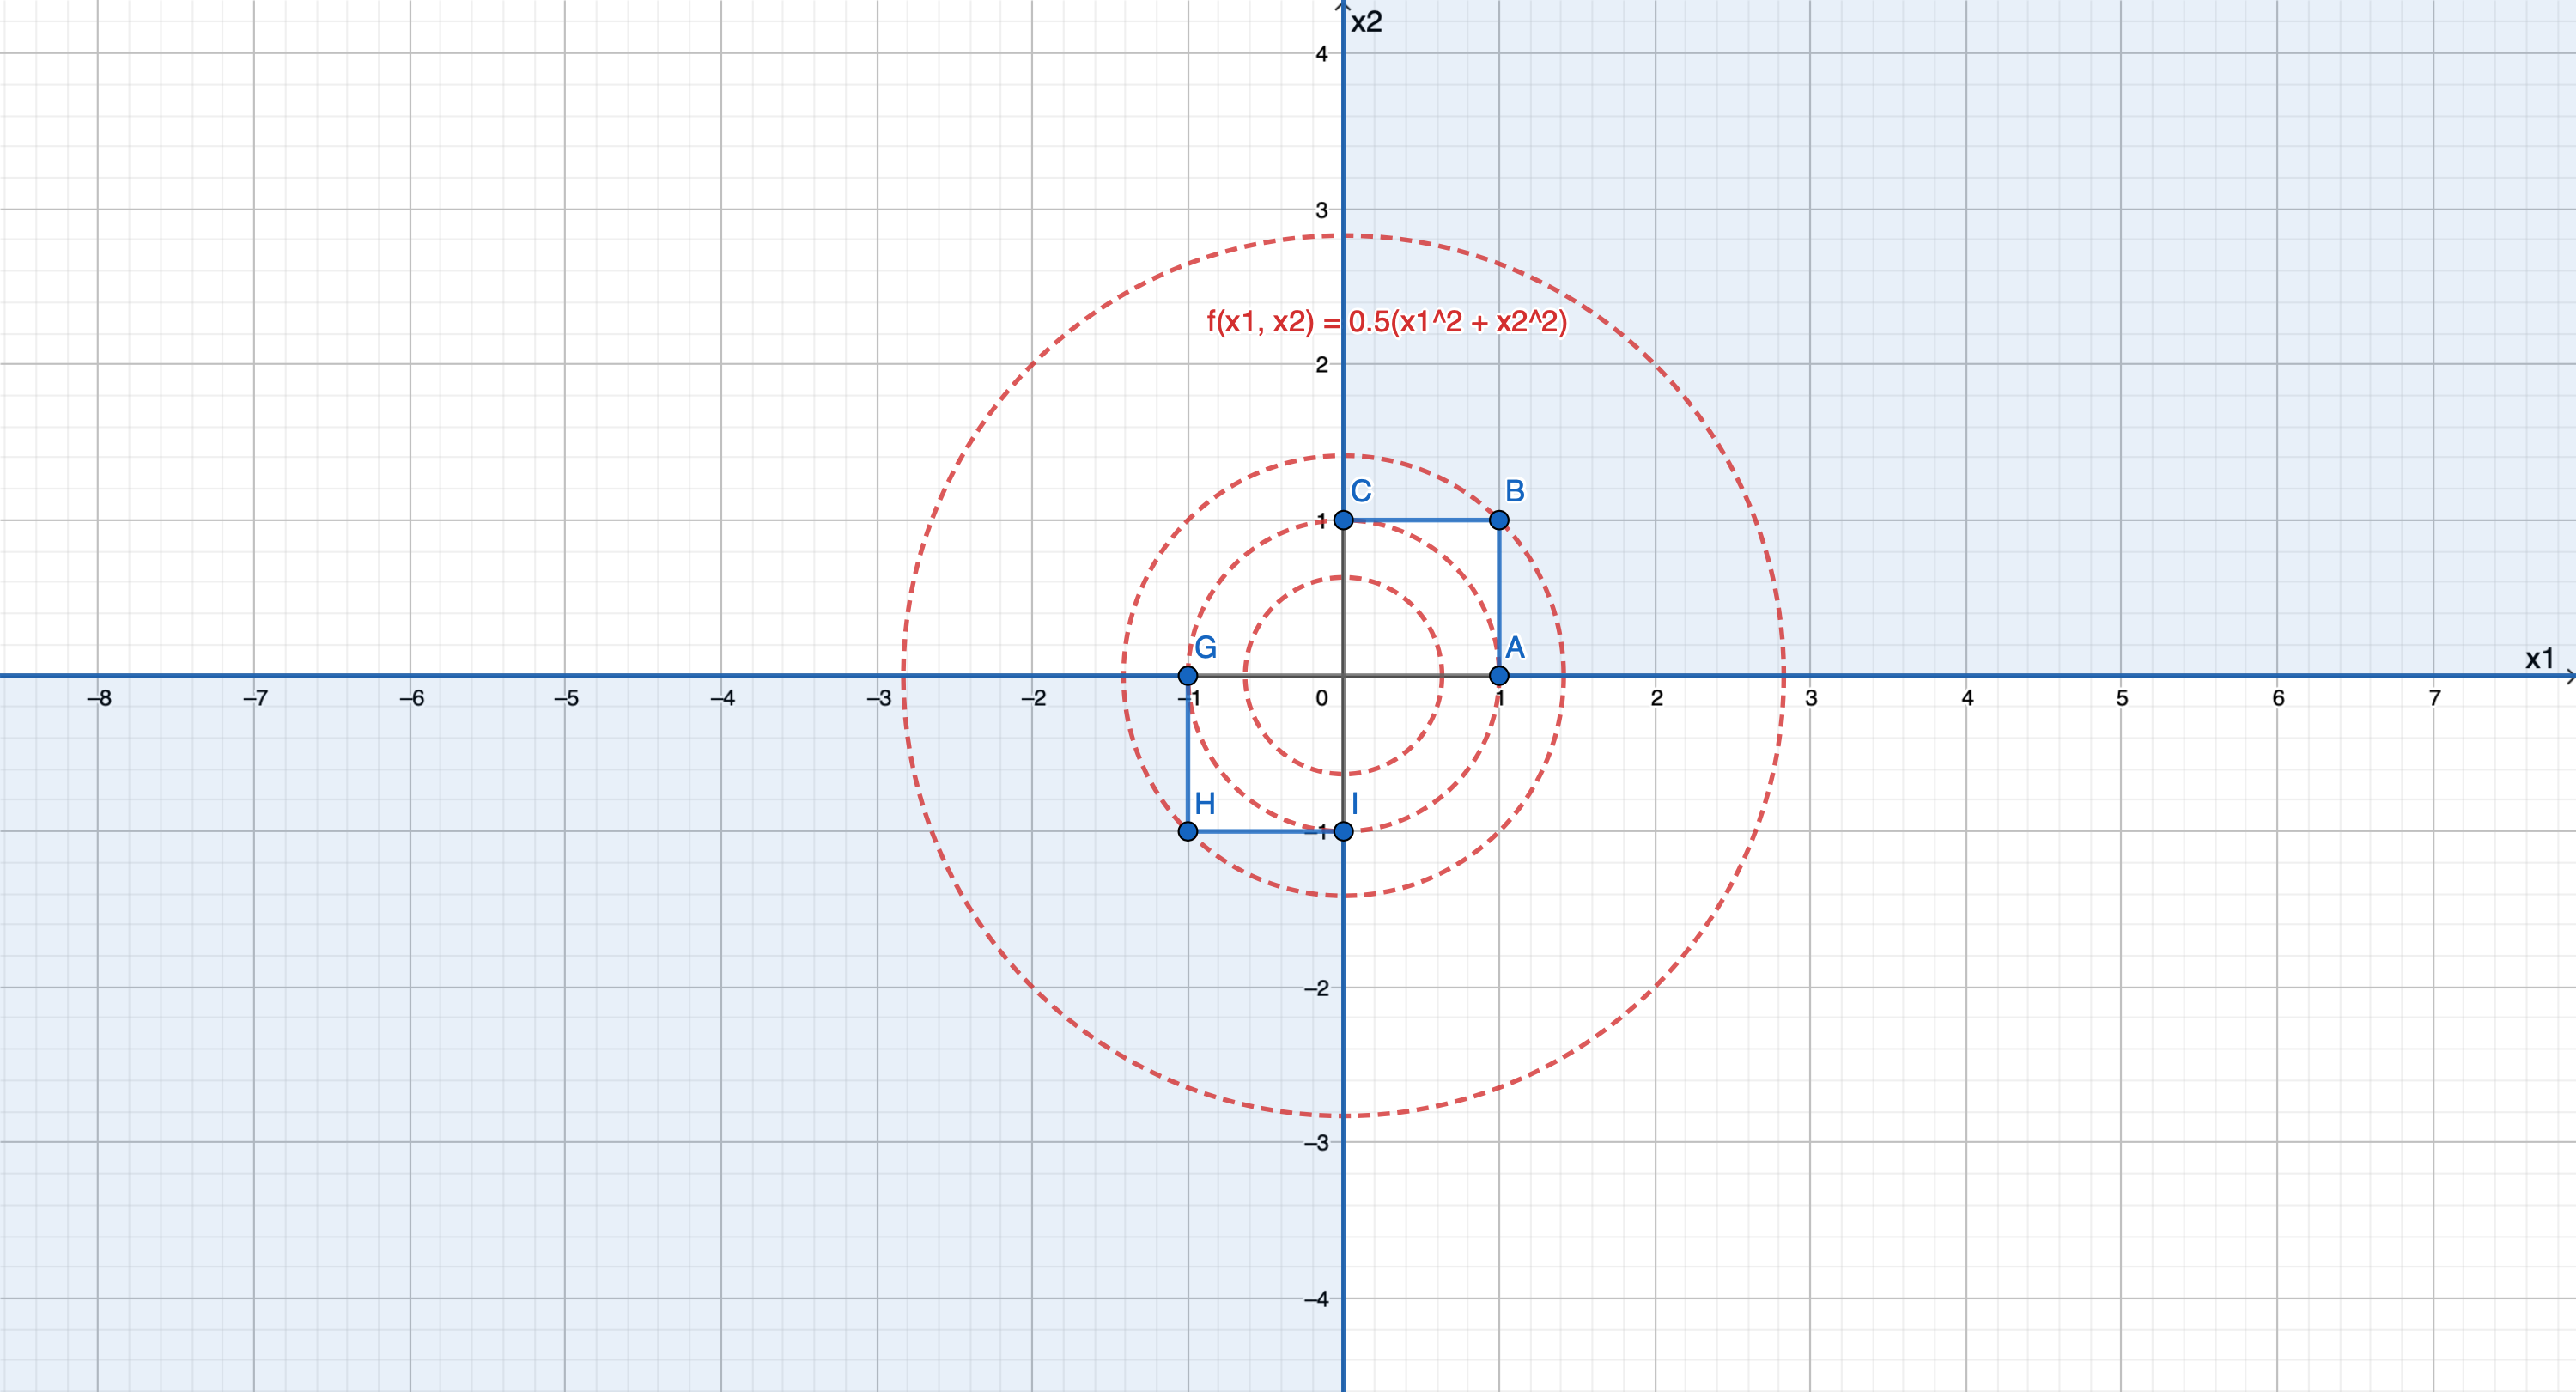
\includegraphics[width=0.55\linewidth]{p5_6}
		\vspace{4pt}
		\caption{$f(\textbf{\textit{x}}) :=\frac{1}{2}(x_1^2+x_2^2)$}
		\label{p5to6}
	\end{figure}
	In order to see the outcome more vividly, we draw the 3D graph of $f(\textbf{\textit{x}})$ as showing in Figure \ref{p5to7}, it can help us to find the minimizer more intuitively.
	\begin{figure}[htbp]
		\centering
		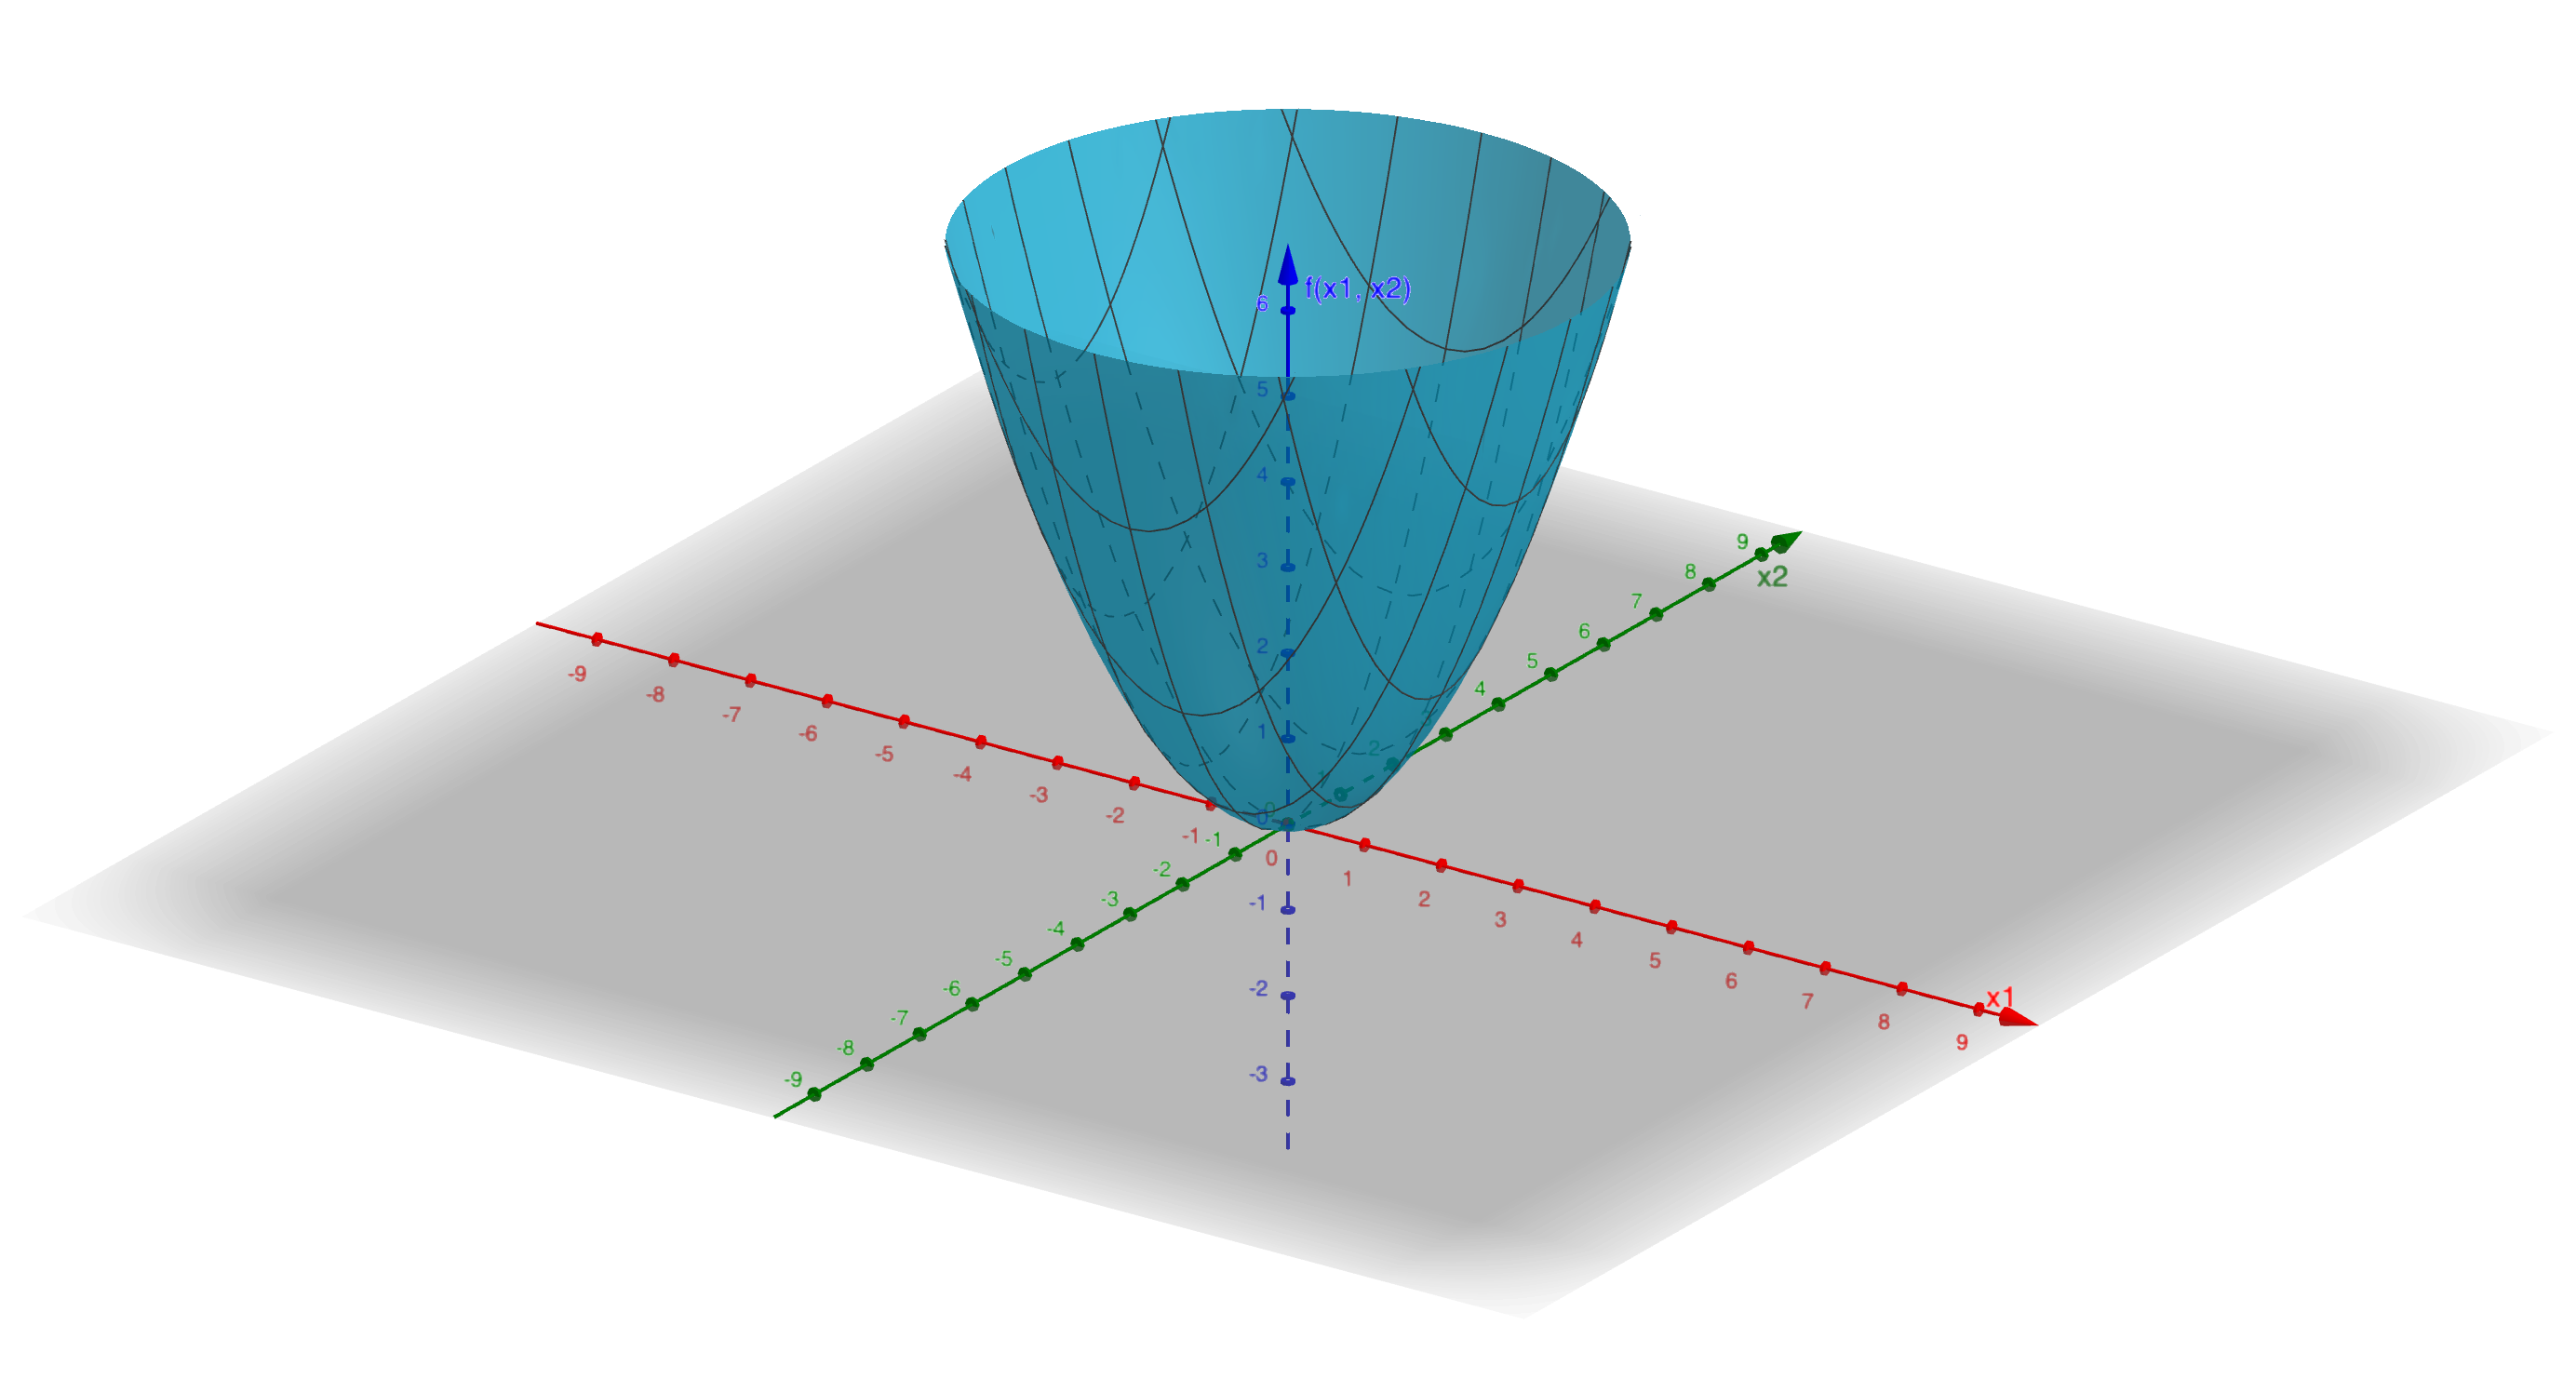
\includegraphics[width=0.5\linewidth]{p5_7}
		\vspace{4pt}
		\caption{The 3D graph of $f(\textbf{\textit{x}})$}
		\label{p5to7}
	\end{figure}
	
	\textbf{Subproblem d)}
	
	The test set $L_\alpha$ is showed by Figure \ref{p5to8}, with differnt $\alpha$, there are different circles (drawed by blue and green dash line) to denote the set $L_\alpha$. The green circle($\alpha=\frac{3}{8}$) is tangent with the function $h(\textbf{\textit{x}})=0$(drawed by red color) at point $A\left(\frac{\sqrt{2}}{2}, -\frac{1}{2}\right)$ and point $B\left(-\frac{\sqrt{2}}{2}, -\frac{1}{2}\right)$. Thus we can find the solution $ \textbf{\textit{x}}^* \in X $ of problem (\ref{p2}) as Point $A\left(\frac{\sqrt{2}}{2}, -\frac{1}{2}\right)$ and point $B\left(-\frac{\sqrt{2}}{2}, -\frac{1}{2}\right)$, which lead the value of $f(\textbf{\textit{x}})$ to be minimum.
	\begin{figure}[htbp]
		\centering
		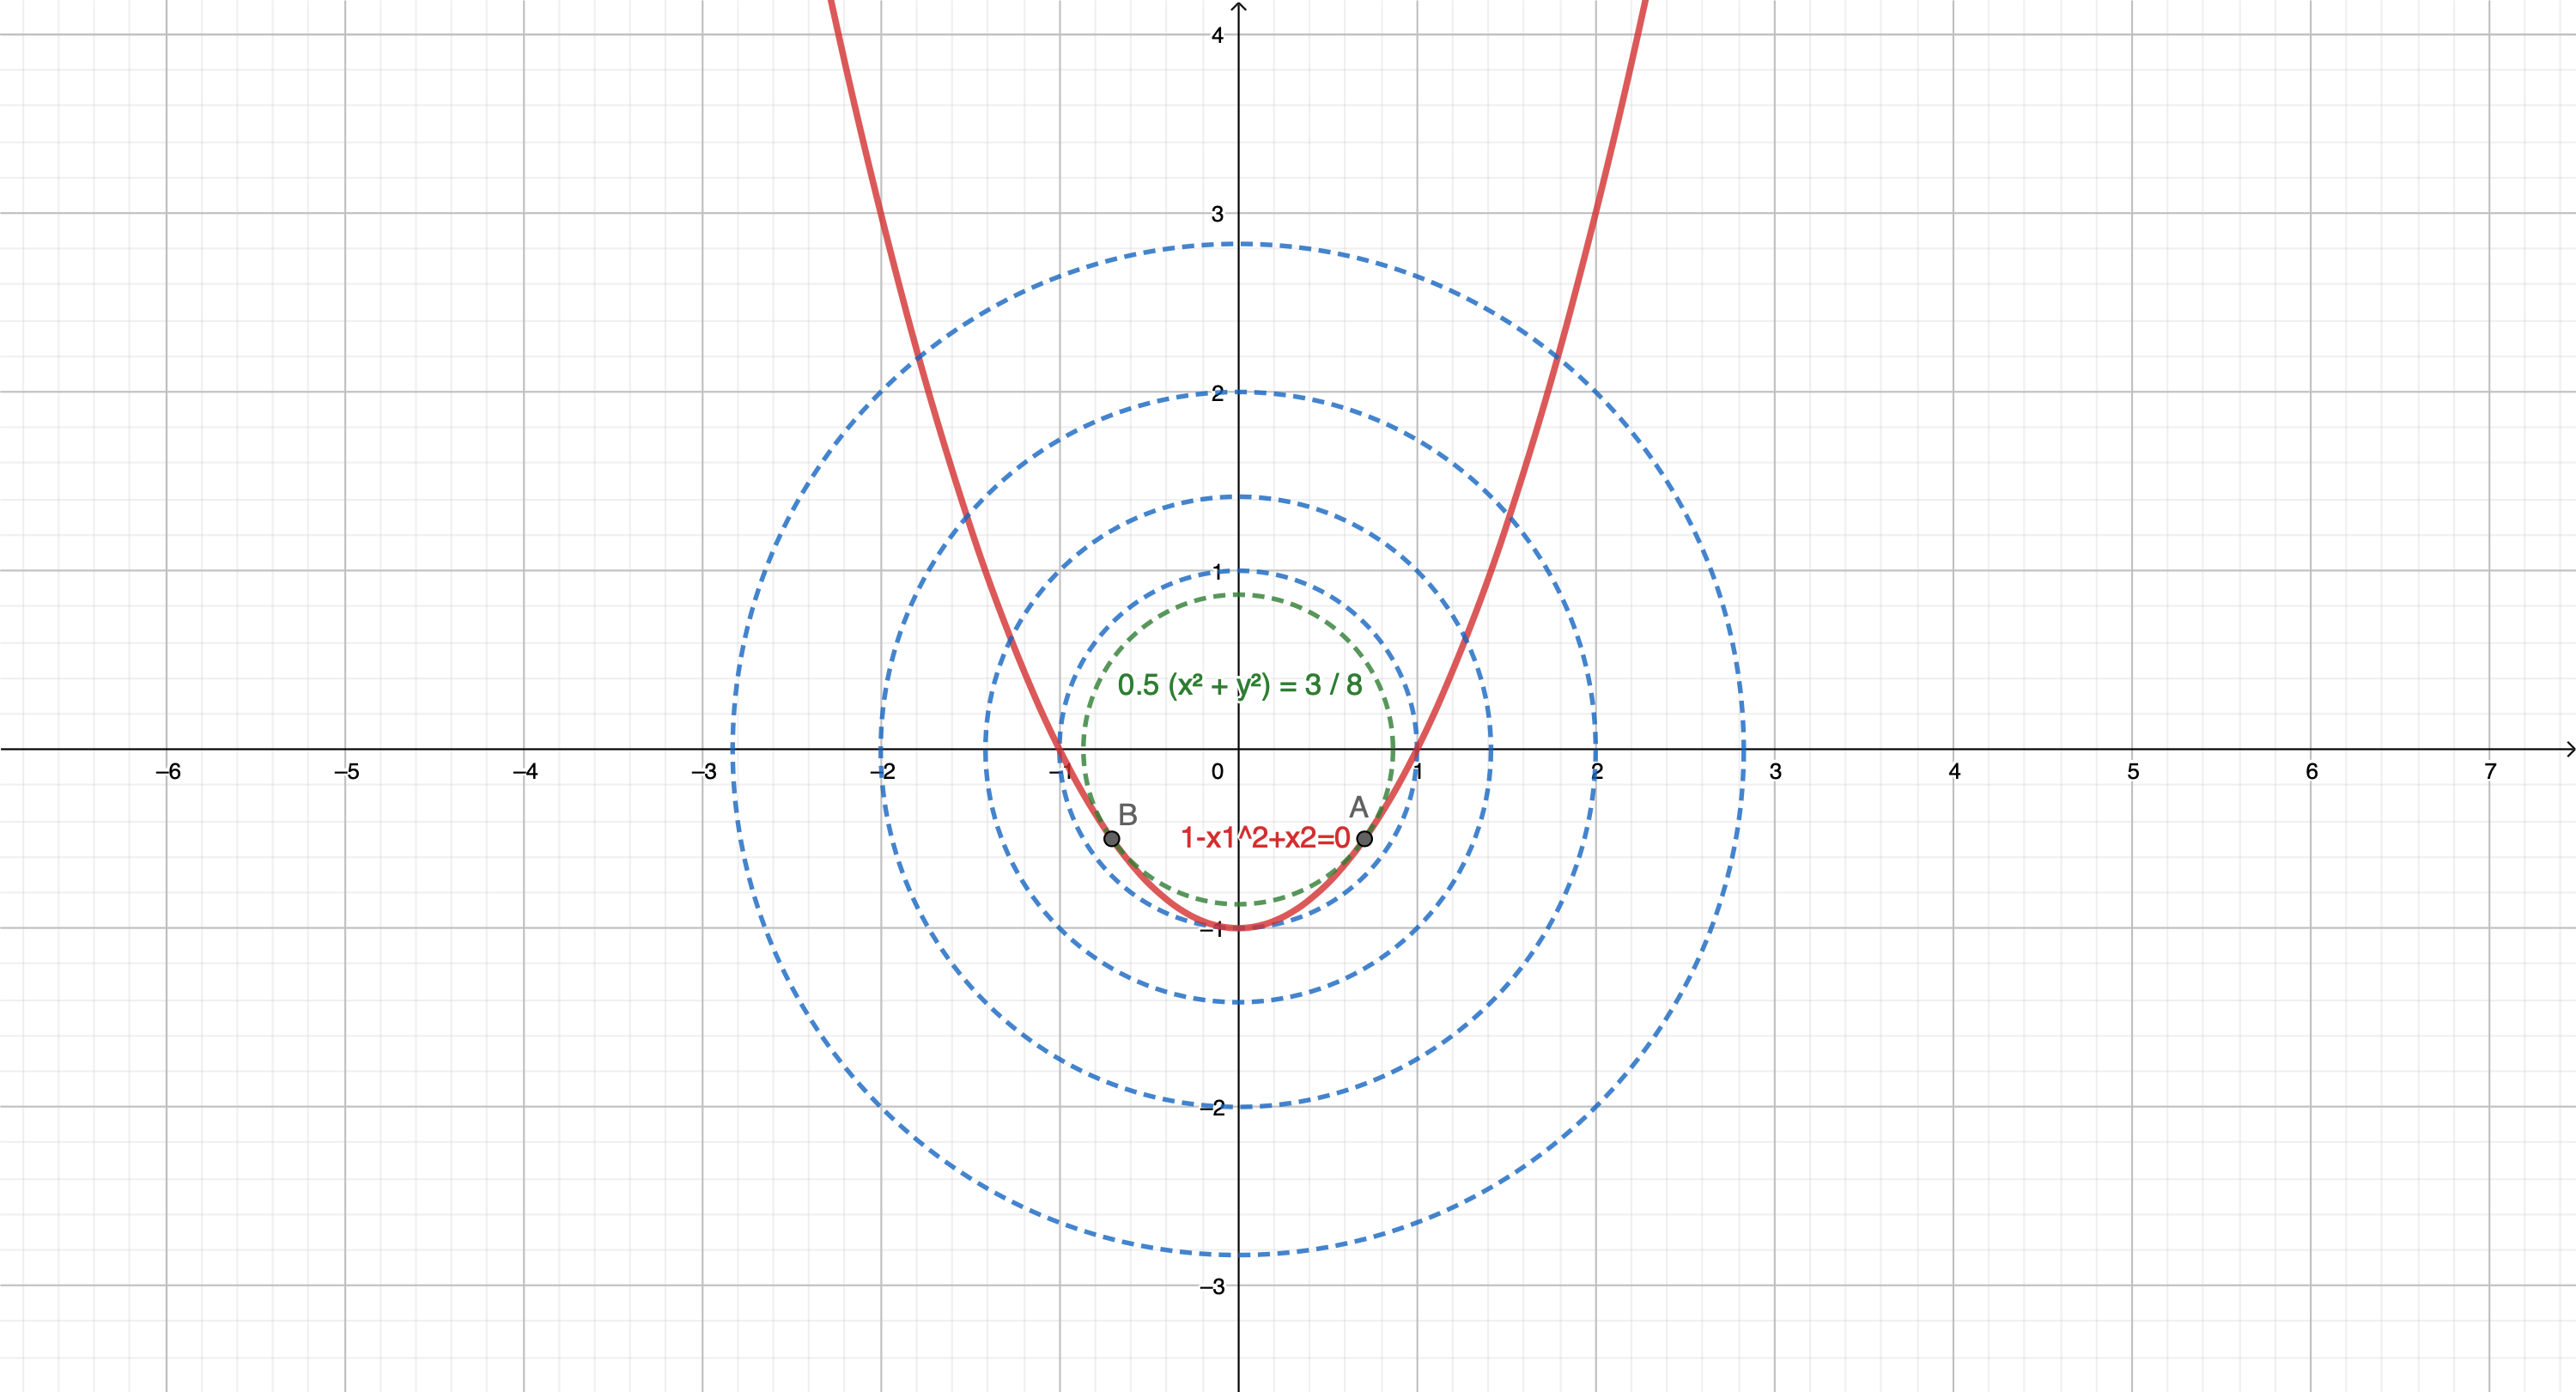
\includegraphics[width=0.6\linewidth]{p5_8}
		\vspace{4pt}
		\caption{$L_\alpha $ and $h(x)=0$}
		\label{p5to8}
	\end{figure}

	\vspace{4pt}
	Because $f(\textbf{\textit{x}}) :=\frac{1}{2}(x_1^2+x_2^2)$ and $h(\textbf{\textit{x}})=1-x_1^2+x_2$, the gradient of $f(\textbf{\textit{x}})$ can $h(\textbf{\textit{x}})$can be derived as
	\begingroup
	\renewcommand*{\arraystretch}{1.5}
	\begin{equation}
		\begin{split}
			\nabla f(x)&=
			\begin{pmatrix}
				\frac{\partial f}{\partial x_1}\\
				\vspace{2pt}
				\frac{\partial f}{\partial x_2}
			\end{pmatrix}
		 	=
		 	\begin{pmatrix}
		 		x_1\\
		 		x_2
		 	\end{pmatrix}
		 	\\
		 	\nabla h(x)&=
		 	\begin{pmatrix}
				\frac{\partial f}{\partial x_1}\\
				\frac{\partial f}{\partial x_2}
		 	\end{pmatrix}
		 	=
		 	\begin{pmatrix}
		 		-2x_1\\1
		 	\end{pmatrix}
		\end{split}
	\end{equation}
	\endgroup
	We have two points ($A$ and $B$) as the $\textbf{\textit{x}}^*$.
	 
	$\circ$ For point $A\left(\frac{\sqrt{2}}{2}, -\frac{1}{2}\right)$, we get the gradient 
	\begingroup
	\renewcommand*{\arraystretch}{1.3}
	\begin{equation}
		\begin{split}
			\nabla f(A)&=
			\begin{pmatrix}
				\frac{\sqrt{2}}{2}\\
				-\frac{1}{2}
			\end{pmatrix}\\
			\nabla h(A)&=
			\begin{pmatrix}
				-\sqrt{2}\\
				1
			\end{pmatrix}
		\end{split}
	\end{equation}
	\endgroup
	We draw the two vectors in Figure \ref{p5to9}, the yellow dash is the vector $ \nabla f(A) $, and the pink dash is the vector $ \nabla h(A) $. We can see that the two vectors are parallel and have opposite direction.
	\begin{figure}[htbp]
		\centering
		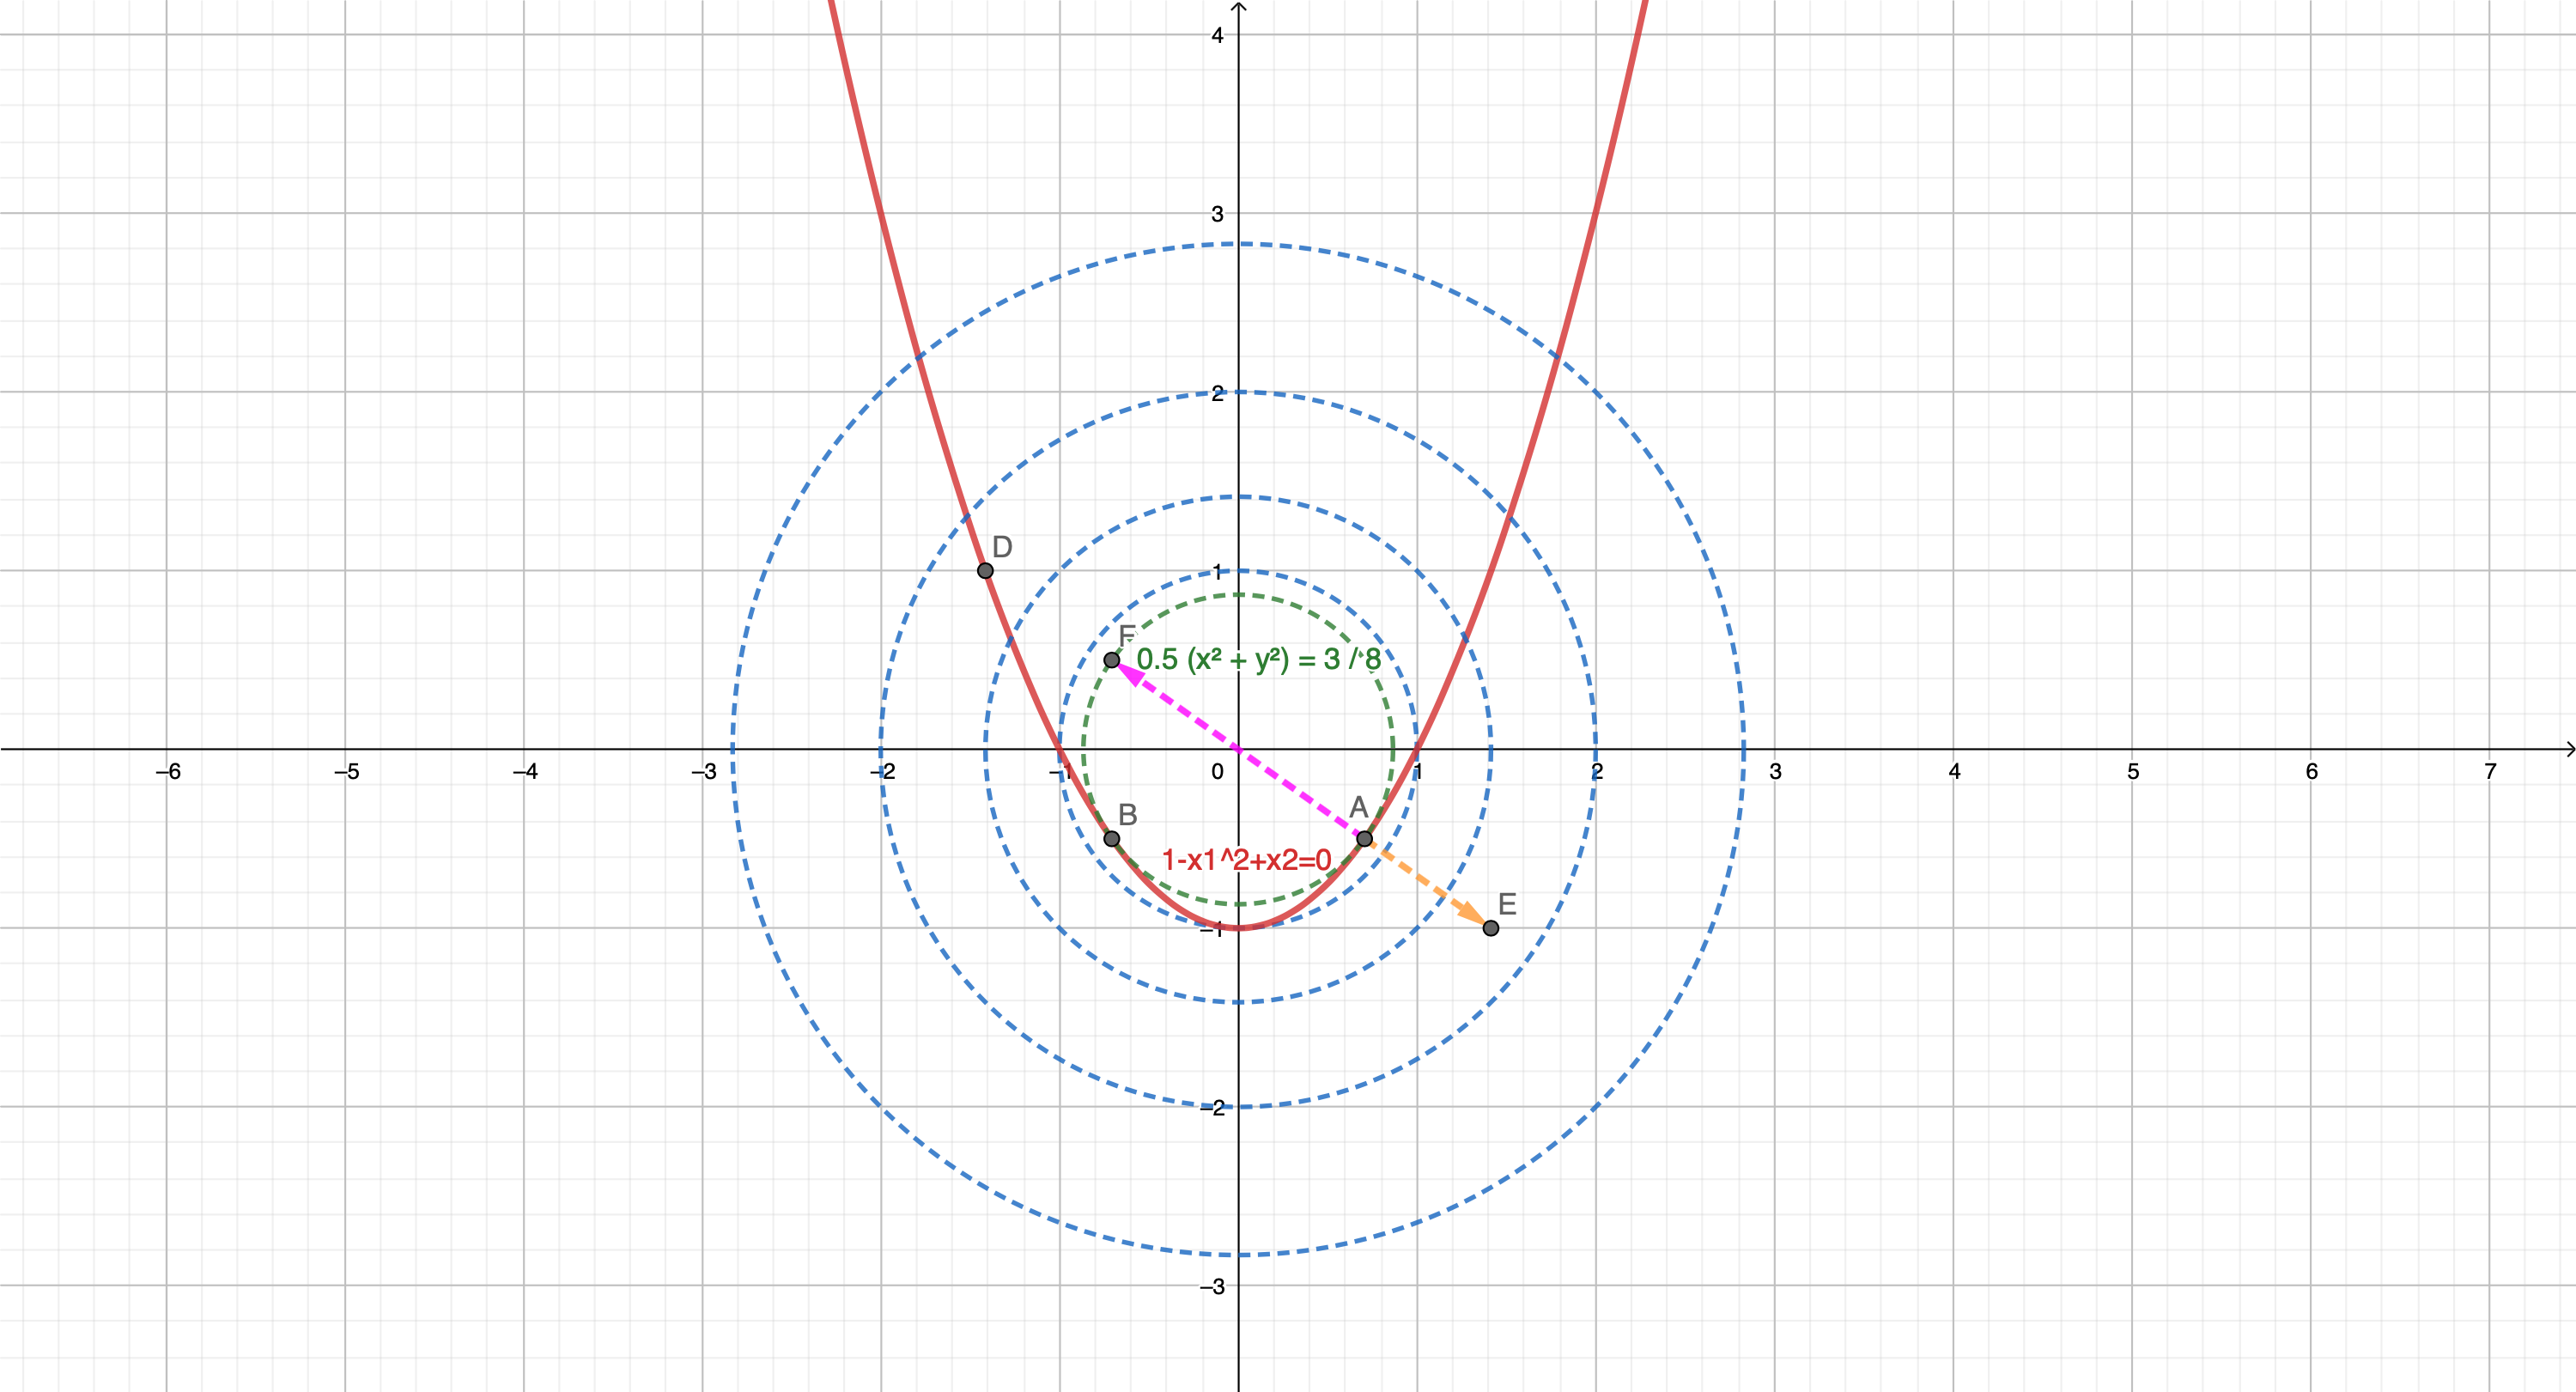
\includegraphics[width=0.6\linewidth]{p5_9}
		\vspace{4pt}
		\caption{$L_\alpha $ and $h(x)$ with gradients}
		\label{p5to9}
	\end{figure}

	$\circ$ For point $B\left(-\frac{\sqrt{2}}{2}, -\frac{1}{2}\right)$, we get the gradient
	\begingroup
	\renewcommand*{\arraystretch}{1.3} 
	\begin{equation}
		\begin{split}
			\nabla f(B)&=
			\begin{pmatrix}
				-\frac{\sqrt{2}}{2}\\
				-\frac{1}{2}
			\end{pmatrix}\\
			\nabla h(B)&=
			\begin{pmatrix}
				\sqrt{2}\\
				1
			\end{pmatrix}
		\end{split}
	\end{equation}
	\endgroup
	We draw the two vectors in Figure \ref{p5to10}, the orange dash is the vector $ \nabla f(B) $, and the pink dash is the vector $ \nabla h(B) $. We can see that the two vectors are parallel and have opposite direction.
	\begin{figure}[htbp]
		\centering
		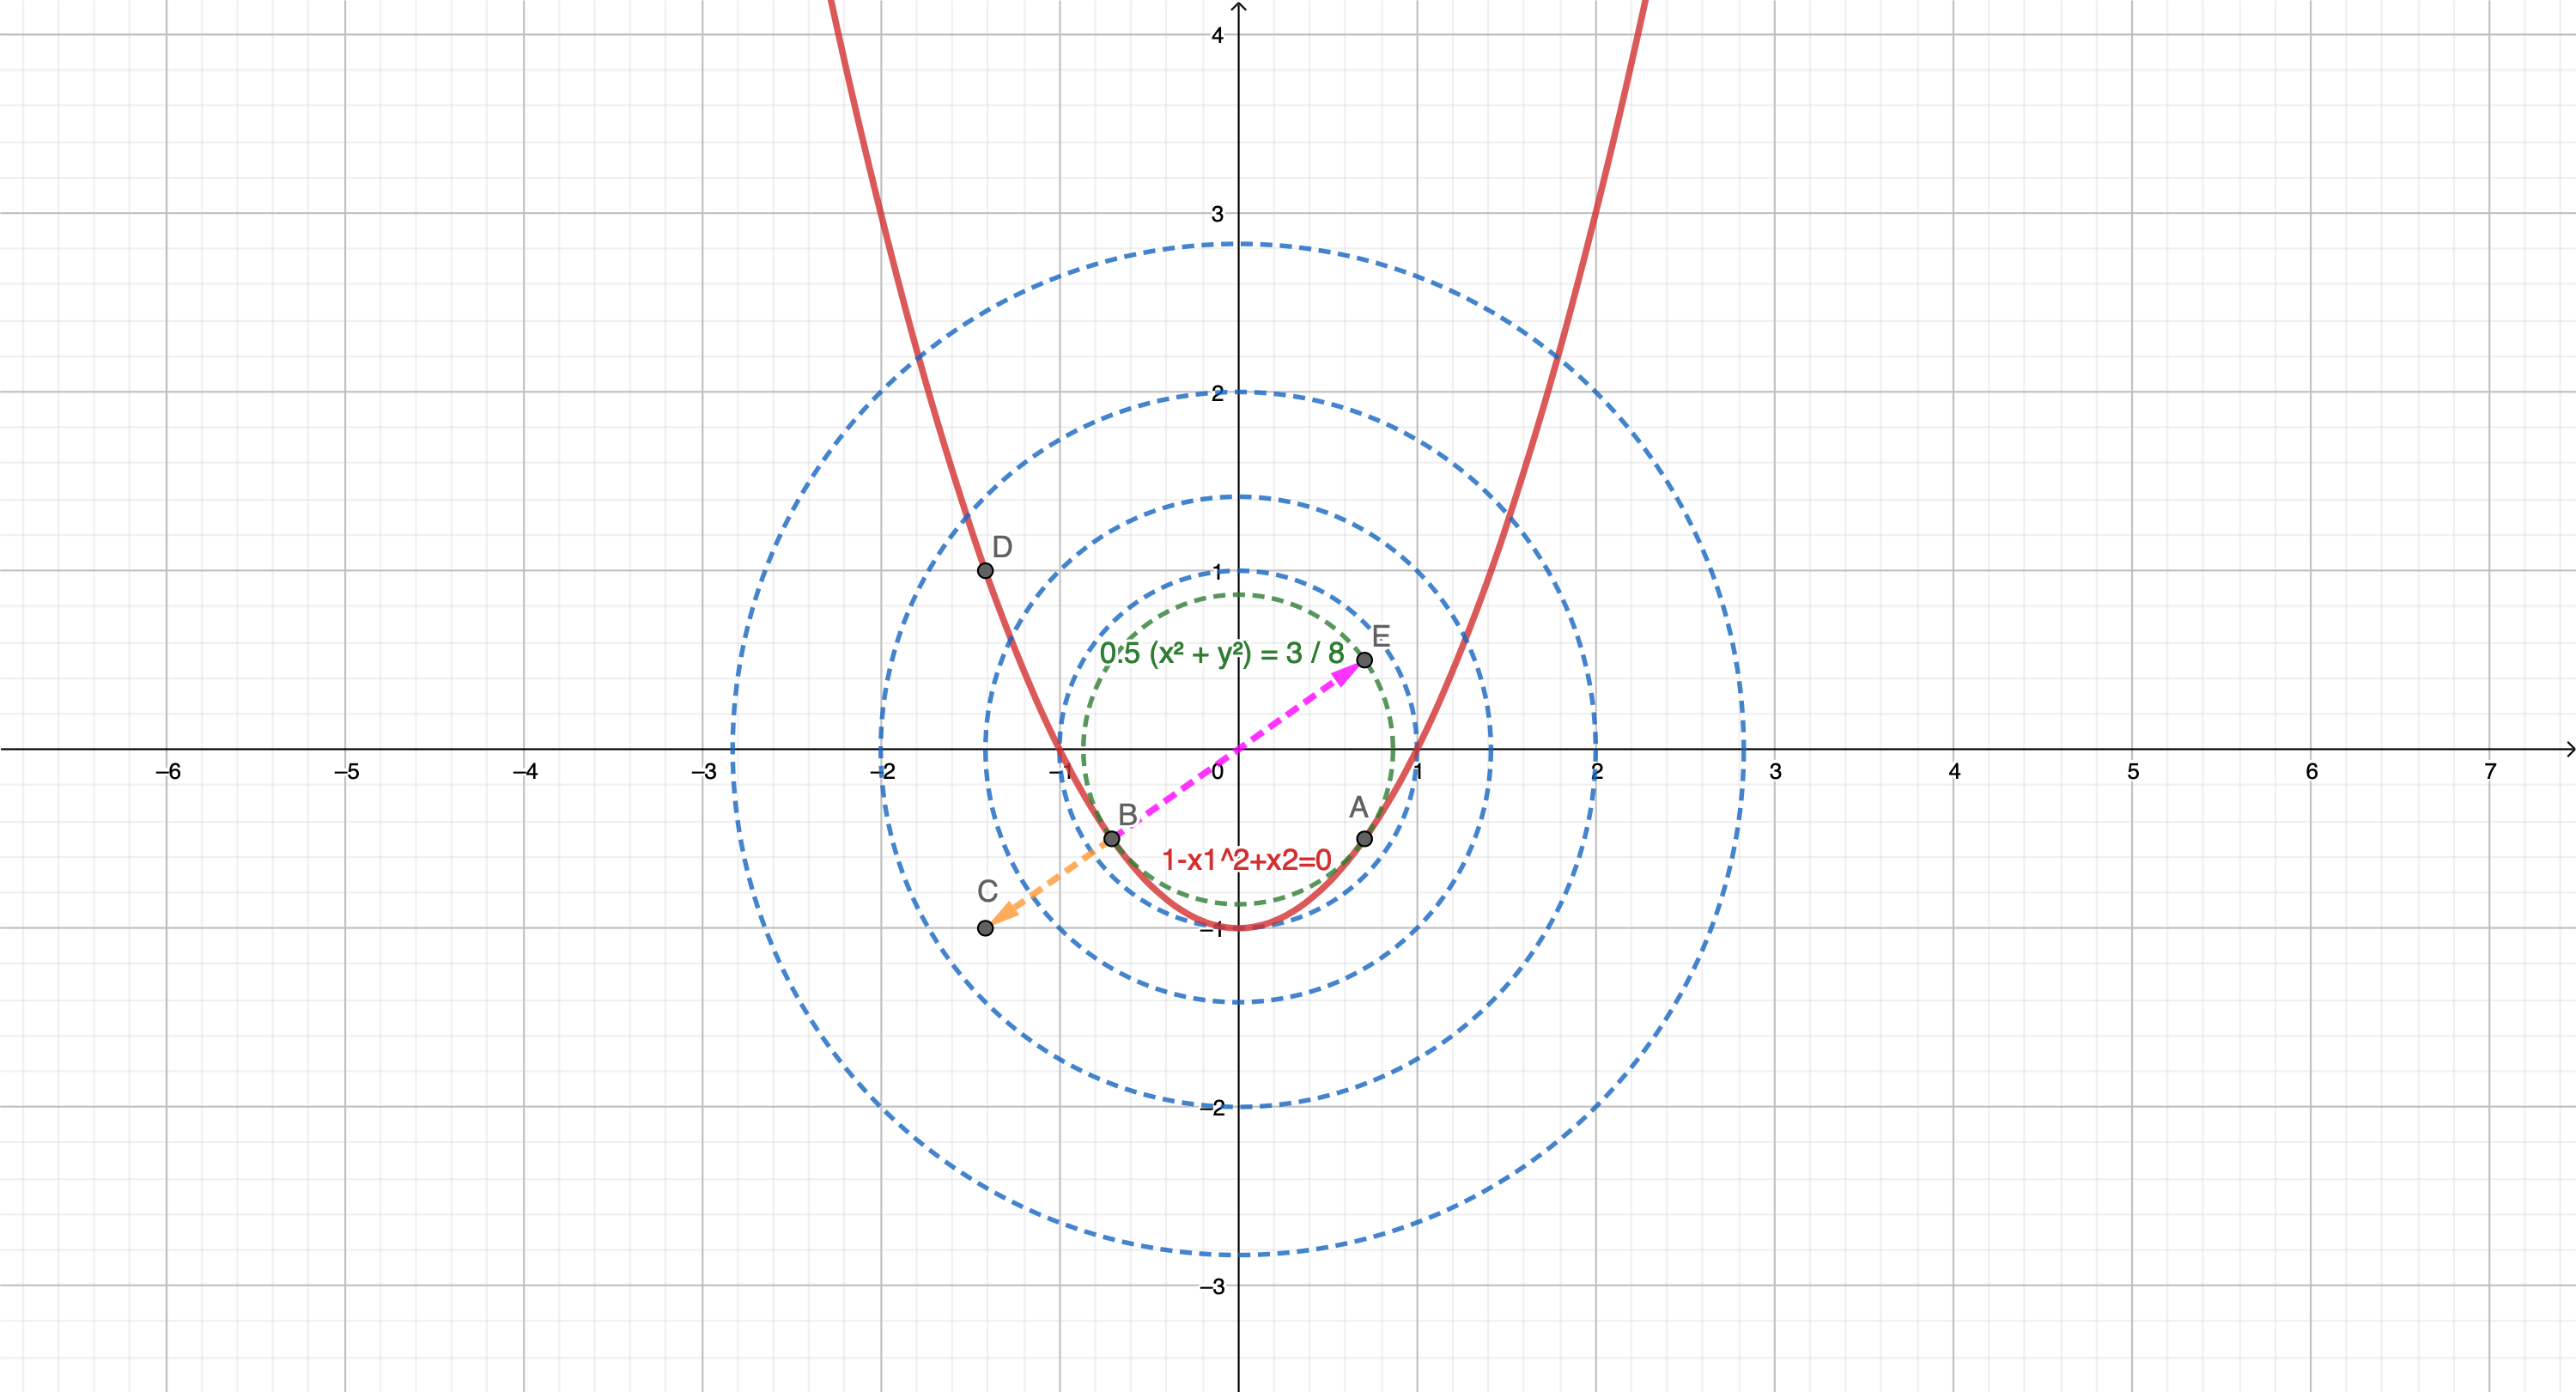
\includegraphics[width=0.65\linewidth]{p5_10}
		\vspace{4pt}
		\caption{$L_\alpha $ and $h(x)$ with gradients}
		\label{p5to10}
	\end{figure}

	Thus, at the point $\textbf{\textit{x}}^*$, the connection between the two vectors $ \nabla f(\textbf{\textit{x}}^*) $ and $ \nabla h(\textbf{\textit{x}}^*) $ is that they are parallel and have opposite direction.
	
	\vspace{4pt}
	
	\textbf{Subproblem e)}
	
	We give the function $f(x)=2x^2-\frac{1}{2}x^3, x\in \mathbb{R}$, and we draw the graph of this function. As we can see from Figure \ref{p5to11}, there is a strict local minimizer $x=0$, as well as the strict local minimum $f(0)=0$. However, there is no global minimum, because when $x\to +\infty$, the value of $f(x)$ will be $-\infty$.
	\begin{figure}[htbp]
		\centering
		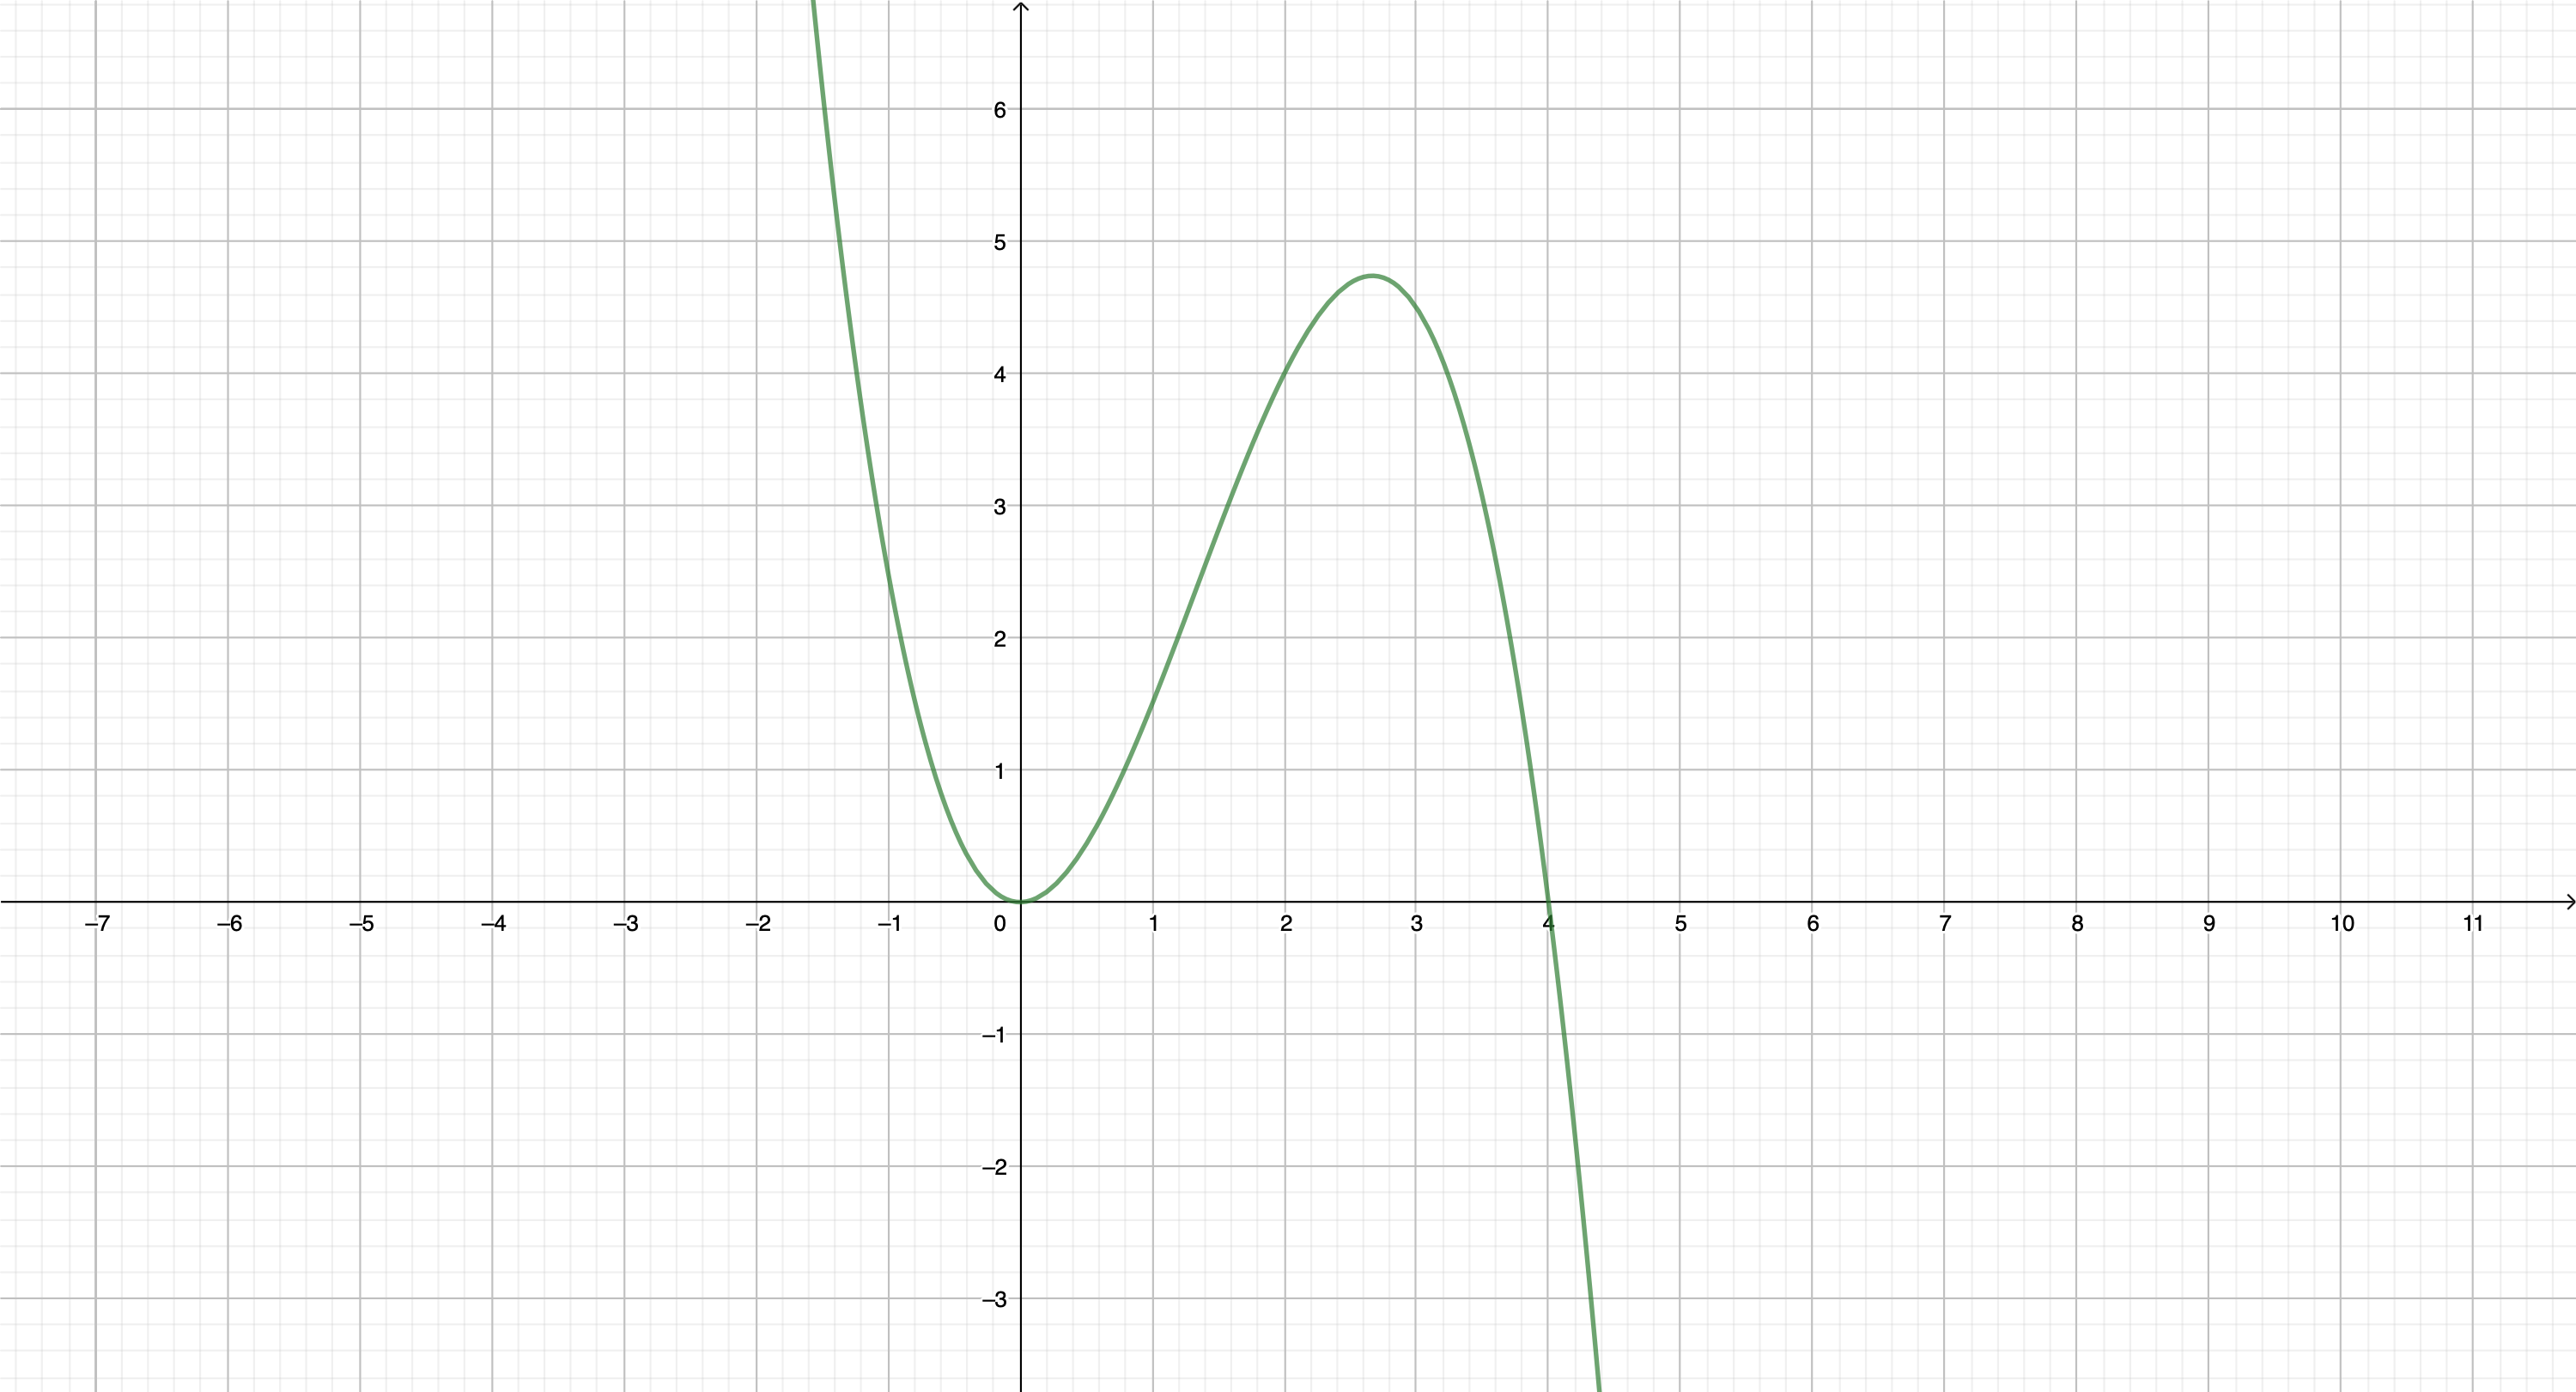
\includegraphics[width=0.65\linewidth]{p5_11}
		\vspace{4pt}
		\caption{Graph of function $f(x)=2x^2-\frac{1}{2}x^3$}
		\label{p5to11}
	\end{figure}
\end{homeworkProblem}
\begin{homeworkProblem}
	In this exercise, we investigate differentiability properties of different functions.
	\begin{enumerate}[\quad a)]
		\item Calculate the gradient and Hessian of the following mappings:
		\begin{equation}
			\begin{split}
			f_1:\mathbb{R}^2\to\mathbb{R},\, f_1(\textbf{\textit{x}})&=(x_1^2-x_2)^2+(x_1-x_2^2)_2-(x_1-1)^3+(x_2-1)^3,\\
			f_2:\mathbb{R}^2\to\mathbb{R},\, f_2(\textbf{\textit{x}})&=\cos(x_1)\sin(x_2)-\frac{x_1}{1+x_2^2},\\
			f_3:\mathbb{R}^2\to\mathbb{R},\, f_3(\textbf{\textit{x}})&=x_1^4+2(x_1-x_2)x_1^2+4x_2^2
			\end{split}
		\end{equation}
		\item Find all points $ \textbf{\textit{x}}^* \in \mathbb{R}^2 $ such that $\nabla f_3(\textbf{\textit{x}}^*) = 0$. Calculate the Hessian $\nabla^2 f_3(\textbf{\textit{x}}^*)$ at those points and investigate the definiteness of the Hessians (i.e., decide whether $\nabla^2 f(\textbf{\textit{x}}^*)$ is positive (semi-)definite, negative (semi-)definite, or indefinite).
		\item Write a MATLAB or Python code to create a 3D-plot (surface plot) and a (two-dimensional) contour plot of the function $ f_3 $. Include the points $ \textbf{\textit{x}}^*$ that you have found in part b) in your plot.
	\end{enumerate}
	\vspace{4pt}
	\textbf{\large{Solution}}
	
	\vspace{4pt}
	\textbf{Subproblem a)}
	
	$\circ$ The gradient of $f_1, f_2, f_3$ can be derived as follow
	\begingroup
	\renewcommand*{\arraystretch}{1.5} 
		\begin{equation}
			\begin{split}
				\nabla f_1(\textbf{\textit{x}})&=
				\begin{pmatrix}
					\frac{\partial f_1}{\partial x_1}\\
					\frac{\partial f_1}{\partial x_2}
				\end{pmatrix}
				=
				\begin{pmatrix}
					4x_1^3-3x_1^2-2x_2^2-4x_1x_2+8x_1-3\\
					4x_2^3+3x_2^2-2x_1^2-4x_1x_2-4x_2+3
				\end{pmatrix}\\
				\nabla f_2(\textbf{\textit{x}})&=
				\begin{pmatrix}
					\frac{\partial f_2}{\partial x_1}\\
					\frac{\partial f_2}{\partial x_2}
				\end{pmatrix}
				=
				\begin{pmatrix}
					-\sin(x_1)\sin(x_2)-\frac{1}{1+x_2^2}\\
					\cos(x_1)\cos(x_2)+\frac{2x_1x_2}{\left(1+x_2^2\right)^2}
				\end{pmatrix}\\
				\nabla f_3(\textbf{\textit{x}})&=
				\begin{pmatrix}
					\frac{\partial f_3}{\partial x_1}\\
					\frac{\partial f_3}{\partial x_2}
				\end{pmatrix}
				=
				\begin{pmatrix}
					4x_1^3+6x_1^2-4x_1x_2\\
					-2x_1^2+8x_2
				\end{pmatrix}
			\end{split}
		\end{equation}
	\endgroup
	$\circ$ The Hessian of $f_1, f_2, f_3$ can be derived as follow
	\begingroup
	\renewcommand*{\arraystretch}{1.5} 
		\begin{equation}
			\begin{split}
				\nabla^2 f_1(\textbf{\textit{x}})&=
				\begin{pmatrix}
					\frac{\partial^2 f_1}{\partial x_1\partial x_1}&
					\frac{\partial^2 f_1}{\partial x_1\partial x_2}\\
					\frac{\partial^2 f_1}{\partial x_2\partial x_1}&
					\frac{\partial^2 f_1}{\partial x_2\partial x_2}
				\end{pmatrix}
				=
				\begin{pmatrix}
					12x_1^2-6x_1-4x_2+8&-4x_2-4x_1\\
					-4x_1-4x_2&12x_2^2+6x_2-4x_1-4
				\end{pmatrix}
				\\
				\nabla^2 f_2(\textbf{\textit{x}})&=
				\begin{pmatrix}
					\frac{\partial^2 f_2}{\partial x_1\partial x_1}&
					\frac{\partial^2 f_2}{\partial x_1\partial x_2}\\
					\frac{\partial^2 f_2}{\partial x_2\partial x_1}&
					\frac{\partial^2 f_2}{\partial x_2\partial x_2}
				\end{pmatrix}
				=
				\begin{pmatrix}
					-\sin(x_2)\cos(x_1)
					&-\sin(x_1)\cos(x_2)+\frac{2x_2}{\left(1+x_2^2\right)^2}\\
					-\sin(x_1)\cos(x_2)+\frac{2x_2}{\left(1+x_2^2\right)^2}
					&-\cos(x_1)\sin(x_2)+\frac{2x_1\left[\left(1+x_2^2\right)-4x_2^2\right]}{\left(1+x_2^2\right)^3}
				\end{pmatrix}
				\\
				\nabla^2 f_3(\textbf{\textit{x}})&=
				\begin{pmatrix}
					\frac{\partial^2 f_3}{\partial x_1\partial x_1}&
					\frac{\partial^2 f_3}{\partial x_1\partial x_2}\\
					\frac{\partial^2 f_3}{\partial x_2\partial x_1}&
					\frac{\partial^2 f_3}{\partial x_2\partial x_2}
				\end{pmatrix}
				=
				\begin{pmatrix}
					12x_1^2+12x_1-4x_2&-4x_1\\
					-4x_1&8
				\end{pmatrix}
			\end{split}
		\end{equation}
	\endgroup
	
	\vspace{4pt}
	\textbf{Subproblem b)}
	
	We set $\nabla f_3(\textbf{\textit{x}}^*)=\textbf{\textit{0}}$, so we can derive $\textbf{\textit{x}}^*$.
	
	\pagebreak
	\begin{equation}
		\begin{split}
			&\nabla f_3(\textbf{\textit{x}})=
			\begin{pmatrix}
			4x_1^3+6x_1^2-4x_1x_2\\
			-2x_1^2+8x_2
			\end{pmatrix}=\textbf{0}\\
			\Rightarrow &
			\begin{cases}
				4x_1^3+6x_1^2-4x_1x_2=0\\
				-2x_1^2+8x_2=0
			\end{cases}\\
			\Rightarrow &
			\begin{cases}
				x_1=0\\
				x_2=0
			\end{cases} \text{or}\quad
			\begin{cases}
				x_1=-2\\
				x_2=1
			\end{cases}
		\end{split}
	\end{equation}
	Thus, we find all $\textbf{\textit{x}}^*$, say point $A(0, 0)$ and point $B(-2, 1)$. So we can calculate the Hessian matrix at point $A$ and $B$ as follow
	\begingroup
	\renewcommand*{\arraystretch}{1.5}
	\begin{equation}
		\begin{split}
			\nabla^2f_3(A)&=
			\begin{pmatrix}
				\frac{\partial^2 f_3}{\partial x_1\partial x_1}&
				\frac{\partial^2 f_3}{\partial x_1\partial x_2}\\
				\frac{\partial^2 f_3}{\partial x_2\partial x_1}&
				\frac{\partial^2 f_3}{\partial x_2\partial x_2}
			\end{pmatrix}
			=
			\begin{pmatrix}
				12x_1^2+12x_1-4x_2&-4x_1\\
				-4x_1&8
			\end{pmatrix}
			=
			\begin{pmatrix}
				0&0\\
				0&8
			\end{pmatrix}
			\\
			\nabla^2f_3(B)&=
			\begin{pmatrix}
				\frac{\partial^2 f_3}{\partial x_1\partial x_1}&
				\frac{\partial^2 f_3}{\partial x_1\partial x_2}\\
				\frac{\partial^2 f_3}{\partial x_2\partial x_1}&
				\frac{\partial^2 f_3}{\partial x_2\partial x_2}
			\end{pmatrix}
			=
			\begin{pmatrix}
				12x_1^2+12x_1-4x_2&-4x_1\\
				-4x_1&8
			\end{pmatrix}
			=
			\begin{pmatrix}
				20&8\\
				8&8
			\end{pmatrix}
		\end{split}
	\end{equation}
	\endgroup
	$\circ$ \textbf{For point $ A $:} because the Hessian matrix at point $ A $ is a diagonal matrix, we can get the eigenvalues of $\nabla^2f_3(A)$ as $\lambda_1=0,\lambda_2=8$. So $\forall \lambda_i\ge 0$, thus matrix $\nabla^2f_3(A)$ is \textbf{positive semidefinite}.
	
	\vspace{4pt}
	$\circ$ \textbf{For point $ B $:} because the Hessian matrix at point $ B $, say $\nabla^2f_3(B)$ is a real symmetric matrix, we can use the eigenvalues of $\nabla^2f_3(B)$ to judge the definiteness of matrix $\nabla^2f_3(B)$.
	
	The characteristic polynomial of $\nabla^2f_3(B)$ can be derived as follow
	\begin{equation}
		\begin{split}
			\begin{vmatrix}
				\nabla^2f_3(B)-\lambda I
			\end{vmatrix}&=
			\begin{vmatrix}
				20-\lambda & 8 \\ 
				8 & 8-\lambda
			\end{vmatrix}=(\lambda-4)(\lambda-24)
		\end{split}
	\end{equation}
	Thus, the eigenvalues of $\nabla^2f_3(B)$ can be derived as $\lambda_1=4,\lambda_2=24$. So $\forall \lambda_i > 0$, thus matrix $\nabla^2f_3(B)$ is \textbf{positive definite}.
	
	\vspace{4pt}
	\textbf{Subproblem c)}
	
	By using python, we draw the 3D-plot (surface plot)  and the contour plot of the function $ f_3 $ as Figure \ref{fig}. Figure \ref{threeD} is the 3D-plot and Figure \ref{contour} is the contour plot. Points $A$ and $B$ are labeled in the figure.
	
	\vspace{-8pt}
	\begin{figure}[htbp]
		\centering
		\subfigure[3D-plot]{\label{threeD}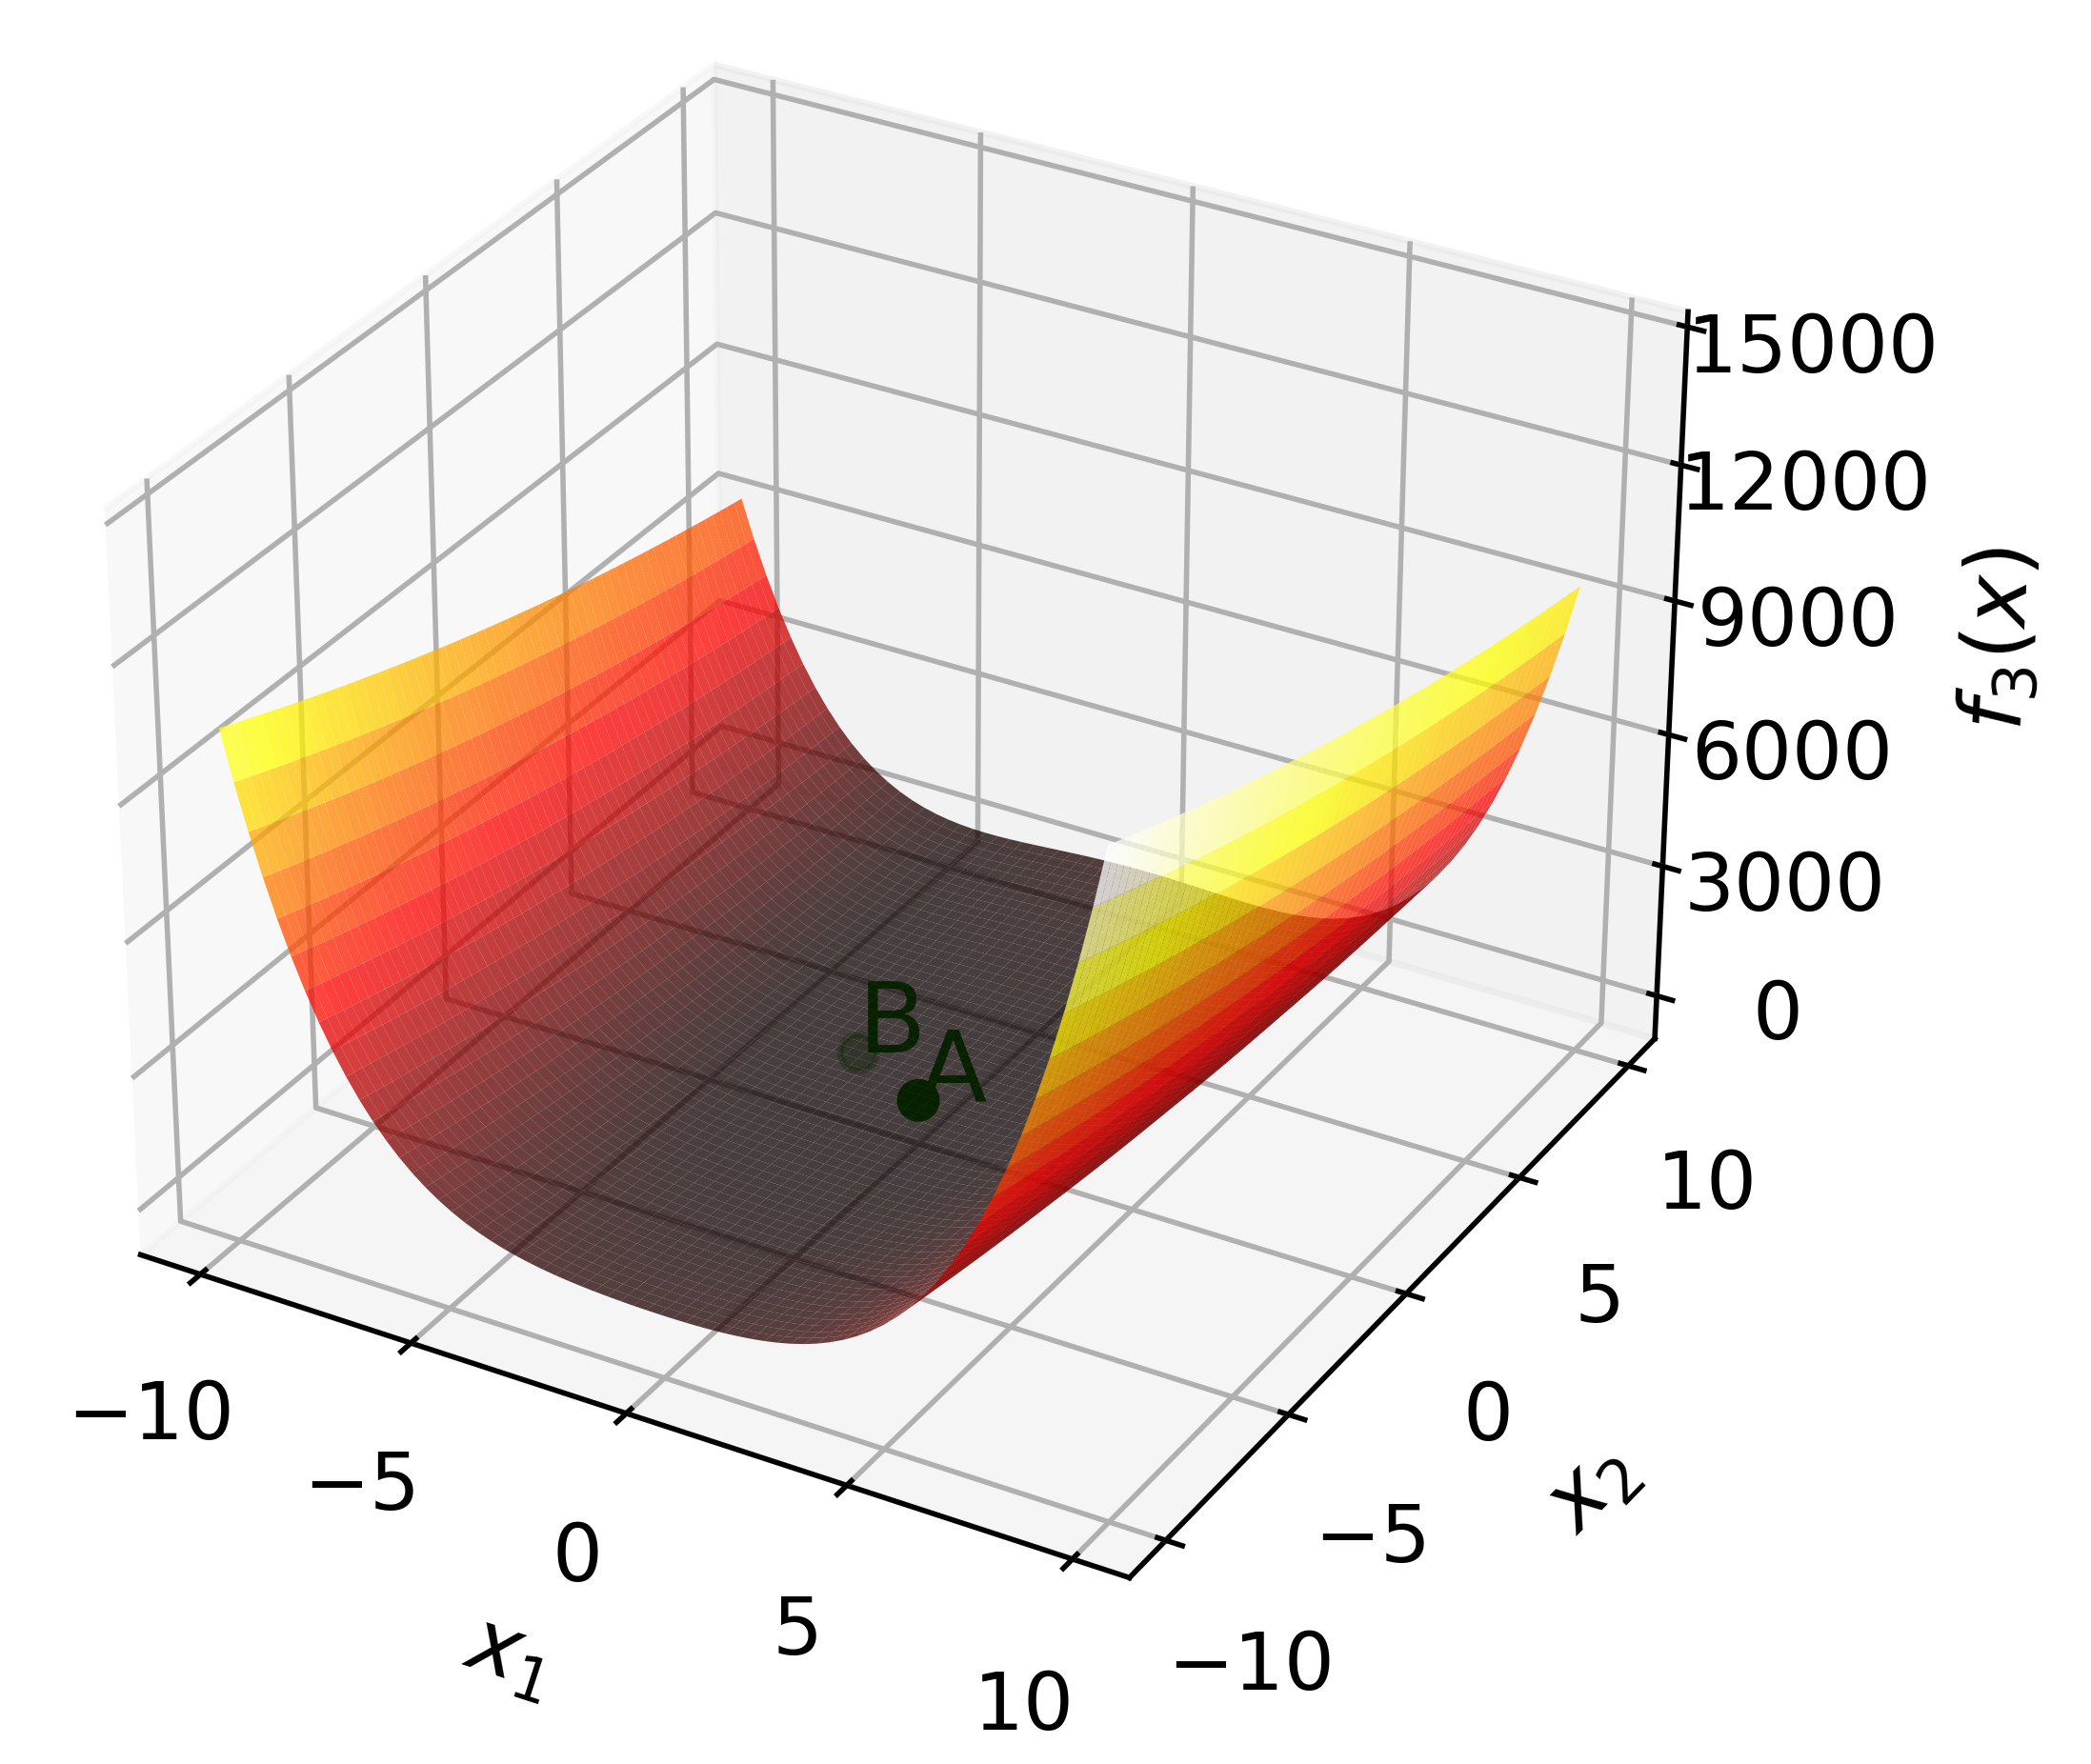
\includegraphics[width=0.41\linewidth]{fig1}}
		\quad
		\subfigure[Contour plot]{\label{contour}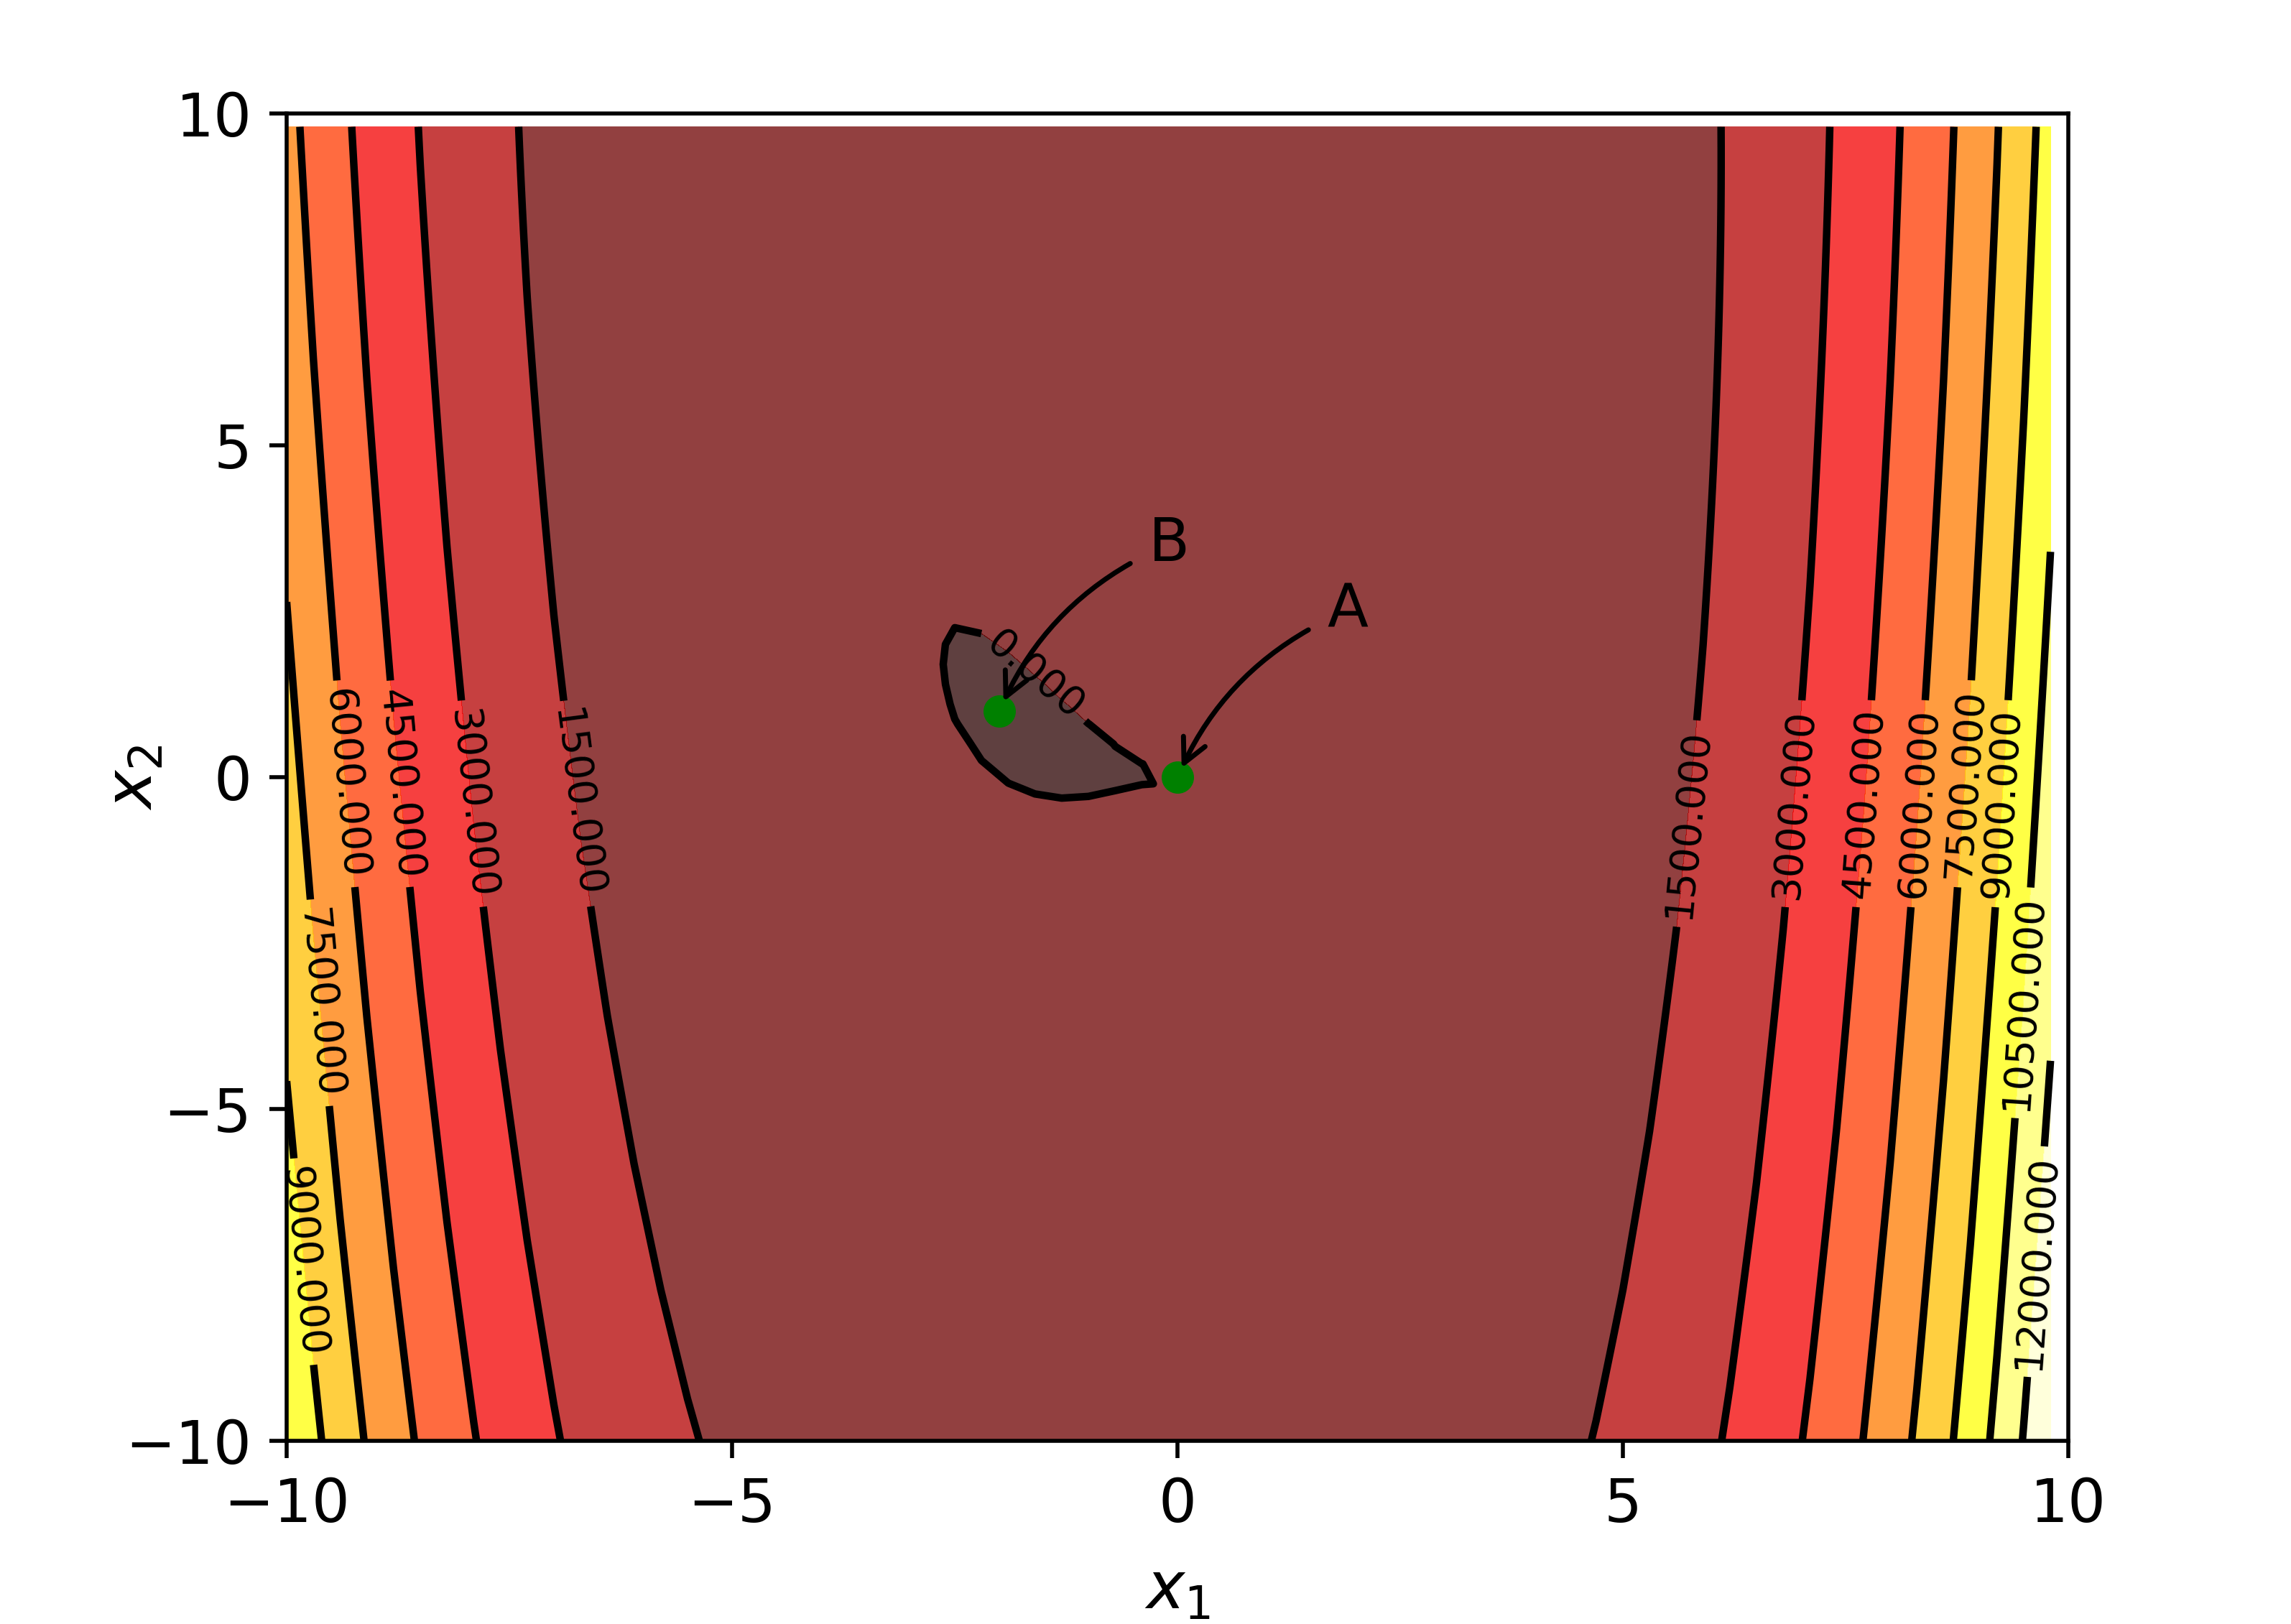
\includegraphics[width=0.5\linewidth]{fig2}}
		\caption{3D and Contour plot of $ f_3 $}
		\label{fig}
	\end{figure}	
\end{homeworkProblem}
\end{document}
